\documentclass[12pt]{colt2020} % Anonymized submission
% \documentclass{colt2020} % Include author names

% The following packages will be automatically loaded:
% amsmath, amssymb, natbib, graphicx, url, algorithm2e

%\usepackage{graphicx}
%\usepackage{amsmath}
%\usepackage{amsthm}
%\usepackage{amssymb}
%\usepackage{thmtools}
\usepackage{mathtools}	
\usepackage{pgfplots}
%\usepackage{hyperref}
%\usepackage{subcaption}
\usepackage{algorithm}
\usepackage{algorithmic}
\usepackage{tikz}

\DeclareMathOperator*{\argmax}{arg\,max}
\DeclareMathOperator*{\argmin}{arg\,min}
\DeclareMathOperator{\E}{\mathbb{E}}
\DeclareMathOperator{\p}{\mathbb{P}}




\title[UCB with an optimal inequality]{UCB with an optimal inequality}
\usepackage{times}
% Use \Name{Author Name} to specify the name.
% If the surname contains spaces, enclose the surname
% in braces, e.g. \Name{John {Smith Jones}} similarly
% if the name has a "von" part, e.g \Name{Jane {de Winter}}.
% If the first letter in the forenames is a diacritic
% enclose the diacritic in braces, e.g. \Name{{\'E}louise Smith}

% Two authors with the same address
% \coltauthor{\Name{Author Name1} \Email{abc@sample.com}\and
%  \Name{Author Name2} \Email{xyz@sample.com}\\
%  \addr Address}

% Three or more authors with the same address:
% \coltauthor{\Name{Author Name1} \Email{an1@sample.com}\\
%  \Name{Author Name2} \Email{an2@sample.com}\\
%  \Name{Author Name3} \Email{an3@sample.com}\\
%  \addr Address}

% Authors with different addresses:
\coltauthor{%
 \Name{Mark Burgess} \Email{mark.burgess@anu.edu.au}\\
 \addr Australian National University, Canberra
}

\begin{document}

\maketitle

\begin{abstract}%
Upper confidence bound multi-armed bandit algorithms (UCB) typically rely on concentration inequalities (such as Hoeffding's inequality) for the creation of the upper confidence bound.
Intuitively, the tighter the bound is, the more likely the respective arm is or isn't judged appropriately for selection.
Hence we derive and utilise an optimal inequality.

Usually the sample mean (and sometimes the sample variance) of previous rewards are the information which are used in the bounds which drive the algorithm, but intuitively the more information that taken from the previous rewards, the tighter the bound could be.
Hence our inequality explicitly considers the values of each and every past reward into the upper bound expression which drives the method.

We show how this UCB method fits into the broader scope of other information theoretic UCB algorithms, but unlike them is free from assumptions about the distribution of the data, 
We conclude by reporting some already established regret information, and give some numerical simulations to demonstrate the method's effectiveness.
\end{abstract}

\begin{keywords}%
Bandit Algorithm; Upper Confidence Bounds; Kullback-Leibler divergence%
\end{keywords}

\section{Introduction}

The multi-armed bandit problem (MAB) is a classic example of a scenario that encodes the general dynamic trade-off between exploration and exploitation in artificial intelligence systems.

The scenario consists of a repeated single decision, who's various choices lead the learner to stochastic rewards.
Over time more information is gathered about the rewards of the decisions that are made, until eventually the learner is in a position of choosing the machine that yields the highest average reward to achieve the greatest long-term expected payoff.
The visceral picture of the situation is of a gambler choosing which poker-machine is best to play over some time frame.

There are several methods of learning in this situation such as the classic $\epsilon$-greedy algorithm (and other $\epsilon$ type methods), Softmax technique (aka. Boltzmann exploration), Pursuit Algorithms, Thomson sampling and Reinforcement Comparison (aka Gradient) methods; but we focus specifically on the UCB family of bandit algorithms.

Upper confidence bound (UCB) bandit algorithms are a popular class of methods where the bandit arm (ie. decision) with the highest upper confidence bound (for some confidence level) on its mean is selected each turn, \cite{LAI19854}.
Typical methods of generating confidence bounds rely on various concentration inequalities; and these function as methods of generating conservative confidence intervals that inform the selection process.
%UCB methods can also be tuned by the confidence level of the bounds each turn.

One of the interesting developments among UCB methods is the improvements which are possible by incorporating tighter concentration inequalities.
Classic concentration inequalities such as Hoeffding's inequality, give confidence interval widths on the mean, based simply on the number of reward samples taken and the size of the support of the data.
Whereas some newer concentration inequalities include reward variance information to create a tighter bound. For instances see \cite{maurer2009empirical, audibert2009exploration,carpentier2011upper}. %- and these are called Empirical Bernstein Bounds (EBBs).

It is understood that the more information about the rewards are used in the creation of an upper confidence bound, the more tightly that bound could be created and the more powerful the resulting UCB method might be.
Indeed, there has been experimentation and positive results incorporating more information (such as variance information) into the UCB method; \cite{DBLP:conf/aaai/MukherjeeNSR18}.

This leads naturally to the question of how to develop more powerful concentration inequalities.
Unfortunately there are an array of powerful and divergent approaches - including is the historical class of Chernoff bounds (including Hoeffding's inequalities, Bernstein's inequality, Bennett's inequality etc.) which arise from an application of Markov's inequality (otherwise more directly leading to Chebyshev's inequality) about the moment generating function, there are developments surrounding Entropy methods (\cite{article1111333}), and the use of the Efron-Stein inequality (or broader `jackknife' method - \cite{efron1981}).
What is notable is that all of these techniques use some loosening approximations to develop their respective concentration inequality expressions.

However, some developments (particularly around Optimal Uncertainty Quantification (OUQ)) has motivated research into developing optimal concentration inequalities - and these don't use any approximations whatsoever - and are optimally tight as a result from finding the worst-case probability density functions directly; \cite{doi:10.1137/10080782X,articleasfasfas}.
We take inspiration from these approaches, and in this paper we develop an optimal concentration inequality and show its performance in the context of the UCB method.

The resulting probability bound not only incorporates information about the sample mean and sample variance but all sample central moments implicitly, as it accounts for all the specific values (and their multiplicities) of all historic rewards from the arms.
Our bound directly incorporates all the reward values (without loosening simplifications) into the creation of a probability bound that is perfectly tight and which utilises all available information available to the learner.

The probability bound that we develop is tight over all possible probability distributions of rewards on bounded support, and we show how it fits into a framework of UCB algorithms developed by \cite{cappe2013} called \texttt{KL-UCB} .

%, who's method stems from comparing the Kullback-Leibler divergence between probability distributions.
We finish by giving a quick numerical case study where we compare the effectiveness of our method against some others.

The paper is divided into the following sections: In section \ref{sec:on_probability} we introduce the kind of probability bound we intend to derive, in Sections \ref{sec:the_optimal_bound} and \ref{sec:the_optimal_bound2} we give summary statements of the optimal bound and a UCB algorithm that uses it, in Section \ref{sec:Bernoulli} we show how the UCB algorithm is identical to \texttt{KL-UCB} in context of Bernoulli data, where-after in Section \ref{sec:KL_section} we talk about the relationship with \texttt{KL-UCB} more generally, and Section \ref{sec:conclusion} concludes with some numerical simulations.

The contributions of this paper are:
\begin{itemize}
\item We derive an optimal probability inequality for the mean of a distribution from the sample values, via the empirical likelihood method, and build it into a UCB algorithm.
\item We show how that resulting algorithm is a computable, performant and lossless instance of the \texttt{KL-UCB} framework that is free from the assumption that the rewards belong to any parametric family of distributions.
\end{itemize}

%http://www.incompleteideas.net/book/bookdraft2018jan1.pdf
%http://proceedings.mlr.press/v23/agrawal12/agrawal12.pdf
%http://www.tokic.com/www/tokicm/publikationen/papers/AdaptiveEpsilonGreedyExploration.pdf
%http://ethen8181.github.io/machine-learning/bandits/multi_armed_bandits.html
%http://bretthard.in/post/bandit-algorithms-are-better-than-a-b-tests
%https://cs.nyu.edu/~mohri/pub/bandit.pdf
%https://towardsdatascience.com/13-solutions-to-multi-arm-bandit-problem-for-non-mathematicians-1b88b4c0b3fc
%https://homes.di.unimi.it/~cesabian/Pubblicazioni/ml-02.pdf
%https://www.researchgate.net/publication/326138176_Reducing_Variance_in_Gradient_Bandit_Algorithm_using_Antithetic_Variates_Method
%http://www.ecmlpkdd2013.org/wp-content/uploads/2013/07/289.pdf
%https://www.cs.mcgill.ca/~vkules/bandits.pdf
%
%



\section{Making an optimal concentration inequality}\label{sec:on_probability}

Historical UCB algorithms have relied on the usage of concentration inequalities such as Hoeffding's inequality.
And these concentration inequalities can be interpreted as analytic unconditioned probability statements about the relationship between sample statistics and population statistics or alternatively about sample statistics as conditioned by population statistics, but not conversely (as is sometimes misunderstood) as about population statistics conditioned by sample statistics. (see appendix \ref{appendix:are_not})

We can see in Appendix \ref{appendix1} (or derivations elsewhere), that the derivation of Hoeffding's inequality begins with the assumption of the mean, and then proceeds to develop a probabilistic bounds the sample mean; and this is a legitimate process of develop bounds on the sample mean conditioned on the assumption of the population mean.

To develop an optimal concentration inequality to replace Hoeffding's inequality in UCB algorithms it is therefore legitimate that we ask the same question that Hoeffding's inequality answers: for a specific possible mean of the data distribution, what is the maximum probability of receiving the relevant sample statistics? And the way in which we answer this question is by solving for the maximising probability density function directly.

\section{An optimal concentration inequality for finite values}\label{sec:the_optimal_bound}

For a specific possible mean of the data distribution, what is the maximum probability of receiving the relevant sample statistics?

%The derivation is found in Appendix \ref{appendix:derivation} 
We begin with the assumption that the distribution of the data only features a finite number of values. And since we are interested in using more than just the sample mean (and sample variance) we ask the question about receiving all sample information.
%, with those values being at least as many as (and including) the sample values.

Our question therefore becomes: what probabilities can the values in our distribution have (consistent with a specified distribution mean) to maximise the probability of receiving all the samples that we did (with their values and multiplicities)?
This question is fundamentally a task of maximising an Empirical Likelihood subject to a constraint, and hence an optimisation problem.

For this problem, the qualities of its solution can be intuited, particularly that non-zero probability must be allocated to all the values of the samples (or otherwise the likelihood would straightforwardly be zero), and then perhaps one other extreme point may have some probability to balance the distribution with the specified mean most effectively.
A graph illustrating this intuition is shown in Figure \ref{illustration1}.

In Theorem \ref{big_o_theorem} of the appendix \ref{appendix:derivation} we solve the optimisation problem analytically to show exactly what probabilities the values have, and when and where the other extreme point occurs.
This process of maximising an empirical likelihood is a well known statistical technique - called the Empirical Likelihood method, and our derivation is reminiscent of this classic technique; see \cite{10.1093/biomet/75.2.237}.

\section{The optimal concentration inequality for finite support}\label{sec:the_optimal_bound2}

By maximising the empirical likelihood of receiving the samples, we saw that there was an upper limit on the number of values in the distribution that will be allocated non-zero probability, specifically the number of sample values plus one.
And this fact remains true irrespective of how many values we limit our distribution to support, and irrespective of how those values are arranged or densely packed.
Therefore we propose that the same behaviour occurs in the limit of continuous distributions.

Hence the continuous distribution that maximises the likelihood of drawing specific samples (for a specific distribution mean) is given by a finite summation of delta functions.

If we assume that the distribution only contains values in a specific range (ie. has finite support) then the maximising likelihood is given by the following theorem (see Appendix \ref{appendix:derivation} for full derivation):


\begin{figure}
\centering
\begin{tikzpicture}[scale=1.6]
\draw (-2,0) -- (2,0);
\draw[dotted, smooth, domain=-2:1.7, color=blue, line width=0.15mm] 
    plot (\x,{-0.55/(\x-2)});
\draw (-2,-0.2) -- (-2,0);
\draw (2,-0.2) -- (2,0);


\def\names{{-0.1,0.2,-1.25,0.4,-0.7,-1.5}}
\def\nameh{{0.114942528735632,
0.128205128205128,
0.082304526748971,
0.138888888888889,
0.095238095238095,
0.077519379844961
}}

\foreach \x in {0,...,5} {
\draw (\names[\x],0) -- (\names[\x],\nameh[\x]*5);
\draw	(\names[\x],-0.25) node{{ $a_{\x}$}};
\draw[black,fill] (\names[\x],\nameh[\x]*5) circle (0.20mm);
}

\draw (0.8,-0.1) -- (0.8,0.1);
\draw	(0.8,-0.25) node{{ $\mu$}};

\draw (2,0) -- (2,0.3629*5);
\draw	(2.15,0.0) node{{ $a_j$}};
\draw[black,fill] (2,0.3629*5) circle (0.20mm);

\draw	(-2,-0.35) node{{ $-2$}};
\draw	(2,-0.35) node{{ $2$}};

\end{tikzpicture}
%\caption{For sample points $a_0,\dots,a_5 = \{-0.1,0.2,-1.25,0.4,-0.7,-1.5\}$ each with single multiplicity drawn from a distribution bounded between $-2$ and $2$ with a mean $\mu=0.8$, the probability of the distribution that maximises likelihood is: $0.128,0.082,0.139,0.095,0.078$ probabilities for the sampled values respectively with the probability of drawing the unsampled value $2$ being $0.363$. We also see the probabilities having hyperbolic weighting centered at $G=a_j=2$ }
\caption{For distributions bounded between -2 and 2, with a specified mean $\mu$, the distribution that maximises the likelihood of drawing sample values $a_0,\dots,a_5$ (each with single multiplicity) including the unsampled value 2. We also see the hyperbolic weighting of probabilities centered at 2.}
\label{illustration1}
\end{figure}


\begin{figure}
\centering
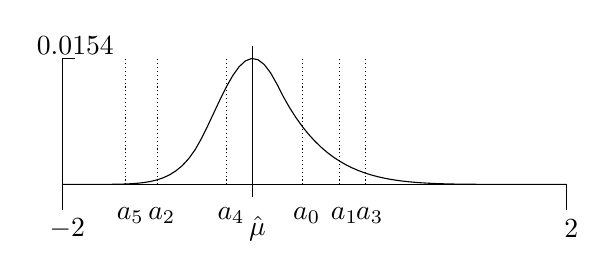
\begin{tikzpicture}[scale=1.6]
\draw (-2,0) -- (2,0);
\draw (-2,-0.2) -- (-2,1);
\draw	(-1.9,1.1) node{{$0.0154$}};
\draw (-2,1) -- (-1.9,1);
\draw (2,-0.2) -- (2,0);


\def\names{{-0.1,0.2,-1.25,0.4,-0.7,-1.5}}

\foreach \x in {0,...,5} {
\draw[densely dotted] (\names[\x],0) -- (\names[\x],1);
\draw	(\names[\x],-0.25) node{{ $a_{\x}$}};
%\draw[black,fill] (\names[\x],1) circle (0.20mm);
}

\draw	(-2,-0.35) node{{ $-2$}};
\draw	(2,-0.35) node{{ $2$}};

\draw (-0.491666,-0.1) -- (-0.491666,1.1);
\draw	(-0.491666,-0.35) node{{ $\hat{\mu}$}};

\draw (-2, 0.0) -- (-1.95, 3.1949045106940002e-09) -- (-1.9, 2.0447388868441601e-07) -- (-1.85, 2.329085388295906e-06) -- (-1.8, 1.308632887580254e-05) -- (-1.75, 4.99203829795935e-05) -- (-1.7, 0.00014906146485093864) -- (-1.65, 0.0003758773207786371) -- (-1.6, 0.0008375250480513626) -- (-1.55, 0.0016979032480677206) -- (-1.5, 0.003194904510693984) -- (-1.45, 0.0056599682298695475) -- (-1.4, 0.009539933750460073) -- (-1.35, 0.015421193846358306) -- (-1.2999999999999998, 0.024056148529832774) -- (-1.25, 0.036391959192123666) -- (-1.2, 0.0536016030752873) -- (-1.15, 0.07711722807528733) -- (-1.1, 0.10866580787633412) -- (-1.0499999999999998, 0.15030709741647255) -- (-1.0, 0.204473888684415) -- (-0.95, 0.27401456684762604) -- (-0.8999999999999999, 0.3620471567576104) -- (-0.8499999999999999, 0.46301593037110456) -- (-0.7999999999999998, 0.5694580368789878) -- (-0.75, 0.6759144001292552) -- (-0.7, 0.7762820274984882) -- (-0.6499999999999999, 0.8642853711025698) -- (-0.5999999999999999, 0.933992911725407) -- (-0.5499999999999998, 0.9803369907493318) -- (-0.5, 0.9995923847771935) -- (-0.44999999999999996, 0.9897691772744265) -- (-0.3999999999999999, 0.9508785474839102) -- (-0.34999999999999987, 0.8850363214801366) -- (-0.2999999999999998, 0.7963785080757475) -- (-0.25, 0.6985028085753533) -- (-0.19999999999999996, 0.6103924216093528) -- (-0.1499999999999999, 0.5317454806837659) -- (-0.09999999999999987, 0.4617307692307688) -- (-0.04999999999999982, 0.39957307361552535) -- (0.0, 0.3445506091008736) -- (0.050000000000000266, 0.2959925063775508) -- (0.10000000000000009, 0.2532763586599564) -- (0.1499999999999999, 0.21582582934744807) -- (0.20000000000000018, 0.1831083202511772) -- (0.25, 0.15463270038646193) -- (0.30000000000000027, 0.12994709533069307) -- (0.3500000000000001, 0.10863673714678175) -- (0.40000000000000036, 0.09032187487213929) -- (0.4500000000000002, 0.07465574557319755) -- (0.5, 0.0613226059654631) -- (0.5500000000000003, 0.050035824599109914) -- (0.6000000000000001, 0.04053603461010866) -- (0.6500000000000004, 0.032589347036891626) -- (0.7000000000000002, 0.025985624702555898) -- (0.75, 0.020536816662602042) -- (0.8000000000000003, 0.016075353218210336) -- (0.8500000000000001, 0.01245260149505354) -- (0.9000000000000004, 0.00953738158764612) -- (0.9500000000000002, 0.00721454326923076) -- (1.0, 0.00538360326720115) -- (1.0500000000000003, 0.003957443104061813) -- (1.1, 0.002861067503924644) -- (1.1500000000000004, 0.0020304233645420757) -- (1.2000000000000002, 0.0014112792948771764) -- (1.25, 0.000958165718210361) -- (1.3000000000000003, 0.0006333755407829468) -- (1.35, 0.0004060253859774359) -- (1.4000000000000004, 0.00025117739403453595) -- (1.4500000000000002, 0.00014902158730697063) -- (1.5, 8.411880105001797e-05) -- (1.5500000000000003, 4.4704179748822446e-05) -- (1.6, 2.205123898245588e-05) -- (1.6500000000000004, 9.896492824733505e-06) -- (1.7000000000000002, 3.924646781789624e-06) -- (1.75, 1.3143562664065307e-06) -- (1.8000000000000003, 3.445506091008709e-07) -- (1.85, 6.132260596546288e-08) -- (1.9000000000000004, 5.383603267201036e-09) -- (1.9500000000000002, 8.411880105001619e-11) -- (2.0, 0.0);

\end{tikzpicture}
\caption{For distributions bounded between -2 and 2 and with the same sample values $a_0,\dots,a_5$ as in figure \ref{illustration1}, the maximum probability that the mean $\mu=x$ consistant with thoes sample values per Theorem \ref{main_theorem}. We see that the maximum height is at the sample mean $\hat{\mu}$ and is very small, and we can see that there is a slightly heavier right side tail as the data samples are left heavy.}
\label{illustration2}
\end{figure}




\begin{theorem}\label{main_theorem}
Over all distributions (bounded between $d^+$ and $d^-$) that have mean $\mu=x$, the likelihood of drawing samples with values $s_1,s_2,s_3,\dots,s_n$ with multiplicities $n_1,n_2,n_3,\dots,n_n$ is least upper bounded by a positive $p_{max}(s_{1..n},n_{1..n}|\mu=x)$.\\
if the sample mean equals the mean (ie. $\hat{\mu} =\sum_in_is_i/(\sum_in_i)=\mu$) then: 
\begin{equation}\label{main_theorem1}p_{max}(s_{1..n},n_{1..n}|\mu=x) = \frac{N!}{\prod_j(n_j!)}\prod_{i=1}^n \left(\frac{n_i}{N}\right)^{n_i}\end{equation}
otherwise:
\begin{equation}\label{main_theorem2}p_{max}(s_{1..n},n_{1..n}|\mu=x) = \frac{N!}{\prod_j(n_j!)}\prod_i \left(\frac{n_i}{N}\frac{G}{G-(s_i-x)}\right)^{n_i}\end{equation}
Where $G$ is constrained such that, $G<\min_i (s_i-\mu)$ or $G>\max_i (s_i-\mu)$\\ and is given by:
$$\left\{
	\begin{array}{ll}
		d^+-x &\mbox{if } \sum_i\frac{n_i(s_i-x)}{s_i-d^+} \ge 0 \\
		d^--x &\mbox{if } \sum_i\frac{n_i(s_i-x)}{s_i-d^-} \ge 0\\
		\mbox{solution of } \sum_i \frac{(s_i-x)n_i}{(s_i-x)-G} =0 &\mbox{otherwise}
	\end{array}
\right.$$
\end{theorem}

As this function $p_{max}$ is parameterised by the mean value $\mu=x$ it is possible to solve and plot it against $x$.
An example plot against $x$ is shown in figure \ref{illustration2} where we can see that the probability profile of the mean indicates that it is most likely about the sample mean, which is what we would expect.

One inconvenience of using this inequality in UCB methods is that the maximum height of the probability profile for $\mu$ does not reach a maximum of $1$.
In the traditional case of Hoeffding's inequality it does reach a maximum of $1$ since it is always perfectly possible that the data distribution has a variance of zero, in which case the mean and sample mean must coincide.
Whereas our inequality considers the spread of sample points more directly, and it is true, that the probability that there is any spread in sample points \textit{and} (or \textit{given that}) the mean has any particular value (or is in any range of values) must be less than one.

However for practical purposes (and this is quite optional) it is convenient to do some scaling to make the probability profile have a height of $1$, and we incorporate this scaling in subsequent Theorem \ref{main_theorem2}.
Additionally, we are primarily interested in the region which the mean exceeds the sample mean ($\mu\ge \hat{\mu}$) by some factor, and one of the easy things to notice is that the maximum point of the profile corresponds to the case $\mu=\hat{\mu}$,
%\footnote{see notes on case1 in Appendix \ref{appendix:derivation}, or otherwise easy to demonstrate}
 and that for $\mu>\hat{\mu}$ that the function is decreasing.
%\footnote{due to submission length limits, the proof of this will have to be left unto the reader}.
And so we convert our function to be an inequality over a range of mean values greater than a parameter $x$, with $\mu\ge x\ge \hat{\mu}$:\footnote{In the same line of reasoning as in Appendix \ref{appendix:are_not}}
$$p_{max}(s_{1..n},n_{1..n},\mu\ge x) = \int_{y\ge x} p_{max}(s_{1..n},n_{1..n}|\mu=y)p(\mu=y)dy $$
$$ \le \max_{y\ge x} p_{max}(s_{1..n},n_{1..n}|\mu=y) = p_{max}(s_{1..n},n_{1..n}|\mu=x)$$
Thus we have converted our inequality which is conditioned by a specific value of the mean, into an unconditioned inequality that is over the range of mean values that we are interested in.
Thus we can restate our Theorem for unit-scaled probability over range of mean values - which coincidentally doesn't need a lower bound anymore:

\begin{theorem}\label{main_theorem_m}
Over all distributions bounded above by $d^+$, that have mean $\mu\ge x$, the unit-scaled likelihood of drawing samples with values $s_1,s_2,s_3,\dots,s_n$ with multiplicities $n_1,n_2,n_3,\dots,n_n$, given that $x>\hat{\mu}$, is least upper bounded by:\\
\begin{equation}\label{main_theorem_m1}p_{max}^{scaled}(s_{1..n},n_{1..n},\mu\ge x) = \prod_i \left(\frac{G}{G-(s_i-x)}\right)^{n_i}\end{equation}
Where $G$ is constrained such that $G>\max_i (s_i-\mu)$, and is given by:
$$\left\{
	\begin{array}{ll}
		d^+-x &\mbox{if } \sum_i\frac{n_i(s_i-x)}{s_i-d^+} \ge 0 \\
		\mbox{solution of } \sum_i \frac{(s_i-x)n_i}{(s_i-x)-G} =0 &\mbox{otherwise}
	\end{array}
\right.$$
\end{theorem}

Working with this measure $p_{max}^{scaled}$ in the context of UCB suggests an like Algorithm \ref{alg2}:

\begin{algorithm}
\caption{UCB operating with $p_{max}^{scaled}$ - \texttt{UCBOI}}
\label{alg2}
\begin{algorithmic}[1]
    \REQUIRE A decreasing function $g:\mathbb{N}\rightarrow\mathbb{R}<1$
	\STATE Pull each of arms $\{1,\dots,K\}$ once
	\STATE thus setting number of pulls for for each arm $a$, $N_a(t)=1$
	\FOR{$t=K$ to $T-1$}
		\STATE for each arm $a$ compute its average historic reward $\hat{\mu}_a$,
		\STATE and compute the $x_a>\hat{\mu}_a$ such that:
$$p_{max}^{scaled}(s_{1..n}^a,n_{1..n}^a,\mu_a\ge x_a) = g(t) $$\vspace{-4mm}%
		\STATE pull an arm $A_{t+1}\in\argmax_{a\in\{1,\dots,K\}}x_a$
	\ENDFOR
\end{algorithmic}
\end{algorithm}

Let us give an example application:

\subsection{The case of Bernoulli data}\label{sec:Bernoulli}

If we are dealing with Bernoulli data then things become a bit simpler and Theorem \ref{main_theorem2} reduces to:

\begin{theorem}\label{main_theorem2}
for Bernoulli distributions that have mean $\mu\ge x$, the scaled likelihood of drawing $n_0$ samples of value $0$ and $n_1$ samples of $1$, if $x>\hat{\mu}$ (with $N=n_0+n_1$), is least upper bounded by:\\
\begin{equation}\label{main_theorem2}p_{max,bernoulli}^{scaled}(n_0,n_1,\mu\ge x) = \left(\frac{1-x}{1-\hat{\mu}}\right)^{n_0}\left(\frac{x}{\hat{\mu}}\right)^{n_1}\end{equation}
\end{theorem}
\begin{proof}
for $s_0,s_1=0,1$ solving $\sum_i \frac{(s_i-x)n_i}{(s_i-x)-G} =0$ gives $G= \frac{\mu(1-x)}{x-\hat{\mu}}$ which is put into equation \ref{main_theorem_m1}. 
\end{proof}

As Algorithm \ref{alg2} runs with a process of finding $x$ such that $p_{max}^{scaled}(\dots,\mu\ge x) = g(t)$, this is much the same thing as finding $x$ such that $\frac{-1}{N}\log p_{max}^{scaled}(\dots,\mu\ge x) = \frac{-1}{N}\log g(t)$ and
$$\frac{-1}{N}\log p_{max,bernoulli}^{scaled} = \hat{\mu}\log\left(\frac{\hat{\mu}}{x}\right) + (1-\hat{\mu})\log\left(\frac{1-\hat{\mu}}{1-x}\right)$$
And this expression might look slightly familiar $\dots$\\ as it is the Kullback-Leibler divergence between the Bernoulli distributions suggested by $\hat{\mu}$ and that is consistent with $\mu=x$.
And if we ran Algorithm \ref{alg2} with Bernoulli data and $g(t) = (t(\log(t))^3)^{-1}$ for $t\ge 3$ with $g(1)=g(2)=g(3)$ we would be running a process equivalent to an instance of \cite{cappe2013}'s \texttt{KL-UCB} algorithm which has been demonstrated to be quite performant.
If we denote the divergence between Bernoulli distributions with means $\mu$ and $\mu'$ as:
$$d_{BER}(\mu,\mu') = \mu\log\left(\frac{\mu}{\mu'}\right) + (1-\mu)\log\left(\frac{1-\mu}{1-\mu'}\right)$$
and if $\mu^\star$ is the maximum mean of the arms (ie. the optimal one) then the regret of the algorithm instance can be characterised by Capp\'{e} et.al's proof that the expected number of pulls of any sub-optimal arm $a$ is bounded by:\\
$ \E[N_a(t)] \le \left(4e + \frac{3}{d_{BER}(\mu_a,\mu^\star)}\right)\log(\log(T)) + \frac{\log(T)}{d_{BER}(\mu_a,\mu^\star)}
 + \frac{2(\log(\mu^\star(1-\mu_a)/(\mu_a(1-\mu^\star))))^2}{(d_{BER}(\mu_a,\mu^\star))^2}
 + 6$\\
\-\hspace{15mm}$ + \frac{\sqrt{2\pi}\log(\mu^\star(1-\mu_a)/(\mu_a(1-\mu^\star)))}{(d_{BER}(\mu_a,\mu^\star))^{\frac{3}{2}}}\sqrt{\log(T)+3\log(\log(T))}$\\

\subsection{A Kullback-Leibler reformulation}\label{sec:KL_section}
The occurrence of the Kullback-Leibler divergence is not coincidence, and if we rearrange equation \ref{main_theorem_m1} we get:
\begin{equation}\label{KL_equation1}-\frac{1}{N}\log p_{max}^{scaled}(s_{1..n},n_{1..n},\mu\ge x) = 
\sum_i\frac{n_i}{N}\log\left(\frac{ \frac{n_i}{N} }{ \frac{n_i}{N}\frac{G}{G-(s_i-x)} }
\right)\end{equation}
Which is the Kullback-Leibler divergence between our derived distribution that maximises likelihood of the samples given a specific mean $x$, and the distribution that is most consistent with those samples, and maximises likelihood irrespective of a specific mean (and occurs when $\hat{\mu}=\mu$).

This then raises the question of exactly where our algorithm and \texttt{KL-UCB} coincide - and the answer is that we believe our algorithm is an unexplored special instance of their more abstract and general framework.
In their more abstract framework they consider a mapping (or a projection operator) $\Pi_\mathcal{D}$ which maps the empirical distribution of the historic rewards of a given arm $\hat{v}_a(t)=\frac{1}{N_a(t)}\sum_{s=1}^t\delta_{Y_s}\mathbb{I}_{A_s=a} $ (which is a sum of Dirac deltas corresponding to rewards) to an element of class $\mathcal{D}$, which is the specific class of distributions that they are considering and comparing via Kullback-Leibler divergences (and potentially needs appropriate selection).
In the application cases that they consider, this mapping mostly occurs via the sample mean - with loss of potential information. Whereas we have created a rather unique case where the this mapping can effectively be the identity - and is therefore lossless as it utilises all available information.

Not only is our algorithm a lossless instance of the \texttt{KL-UCB} framework, but is is also free from any assumptions about the distribution of the data (excepting that is bounded above) whereas all other promoted cases of \texttt{KL-UCB} that are developed into a computable algorithms, assume that the data distribution must be one of a parameterised family of distributions (eg. Bernoulli, Exponential, Poisson, etc) within which the Kullback-Leibler divergences can be computed and expressed. This is a restriction which we seem to have bypassed.

However since our UCB algorithm is an instance of \texttt{KL-UCB} it also inherits some favourable regret bounds, particularly that regret bounds can be derived from the fact that the number of pull of sub-optimal arm $a$ is bounded by:
$$ \E[N_a(t)] \le \frac{\log(T)}{\mathcal{K}_{inf}(\nu,\mu^\star)}(1+o(1)) $$
where $\mathcal{K}_{inf}(\nu,\mu) = \text{inf}\{KL(\nu,\nu'):\nu'\in\mathcal{D}\mbox{ and }E(\nu')>\mu\}$ and reads as the infimum of Kullback-Leibler divergences between the arm distribution $\nu$ and distributions in the model $\mathcal{D}$ that have expectations larger than $\mu$.
Which in our case is given by equation \ref{KL_equation1}.

This expression has been identified as a formula for lower and upper bounds on optimal asymptotic regret of UCB algorithms, see \cite{Maillard11afinite-time}. Additionally there are some other regret expressions that our algorithm tacitly inherits, such as given by \cite{5b3d98cc17c44a510f801b3f}, as the analysis and performance of information theoretic UCB algorithms is an area of research. However in order witness how effective our algorithm is in practice, it is simple enough to run some experiments.

\section{Concluding experiments}\label{sec:conclusion}

Let us conclude with some numerical experiments.\footnote{Github URL to be inserted here in the final version, for reproducible results}
In Figure \ref{biggraph44}, we plot the average cumulative regret over bandit simulations with $5$ arms. We considered:
\begin{itemize}
\item a UCB1 algorithm (developed in \cite{Auer2002}) which chooses the arm with the highest sample mean of $n$ historic rewards plus $\sqrt{2\log(t)/n}$
\item an untuned UCB-V algorithm (given in \cite{audibert2009exploration}) which chooses the arm with highest sample mean plus $ \sqrt{2\hat{\sigma}^2\log(t)/n}+\sqrt{\log(t)/n} $ (where $\hat{\sigma}^2$ is the biased sample variance of past rewards)
\item our own algorithm \ref{alg2} with $g(t) = (t(\log(t))^3)^{-1}$ and 
\item also a method of random arm pulling.
\end{itemize}
\noindent
In Figure \ref{biggraph44} we considered different distributions of rewards for the arms. particularly, we considered:
\begin{enumerate}
\item Beta distributed rewards parameterised by $\alpha$ and $\beta$ parameters were uniformly randomly generated between $0.1$ and $3.1$
\item We also considered uniform distributed rewards where the two poles of the reward were uniformly generated to be within the interval $[0,1]$
\item We also considered Triangularly distributed rewards, where mode of the triangle was randomly generated to be within the interval $[0,1]$ and where its bounds were $0,1$
\item We also considered Trapezoidally distributed data, where the data spans the range $[0,1]$ and the density is flat between two poles uniformly generated within the range $[0,1]$
\end{enumerate}
\noindent
From these graphs we can see our method performs well across a range of possible data.

\begin{figure}[t]
\centering
    \subfigure[]%
{\resizebox{0.5\linewidth}{!}{%beta
	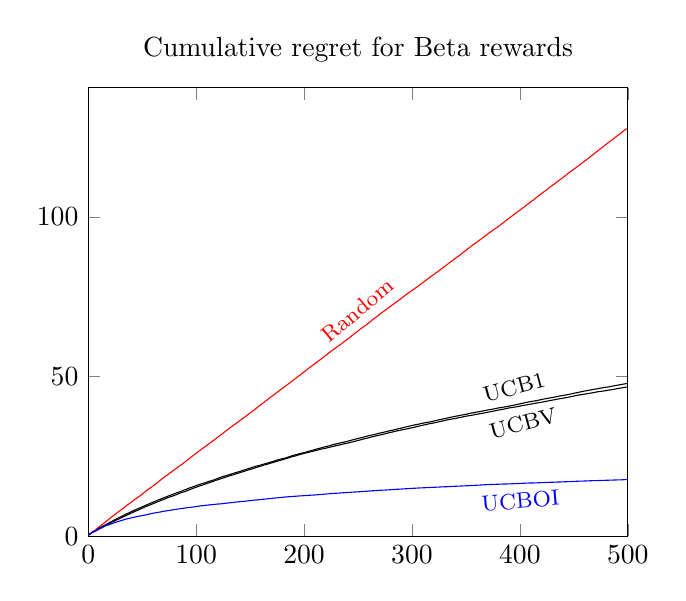
\begin{tikzpicture}
	\begin{axis}[
		title={Cumulative regret for Beta rewards},
		%xlabel={Total number of pulls},
		xmin=0, xmax=500,
		ymin=0, %ymax=20,
	%	ymajorgrids=true,
		grid style=dashed
	]
	\addplot[red] coordinates {
(0,0.279533335201)(1,0.557549655693)(2,0.796953654567)(3,1.0600916165)(4,1.32459869808)(5,1.57131065121)(6,1.80523530514)(7,2.05799975829)(8,2.34176270402)(9,2.65090614206)(10,2.86977355523)(11,3.11577837627)(12,3.38436948269)(13,3.62848087774)(14,3.93159364788)(15,4.2155493193)(16,4.4642756019)(17,4.71922811152)(18,5.01032427666)(19,5.28975347958)(20,5.55136857955)(21,5.82755691276)(22,6.07471882702)(23,6.33649075115)(24,6.59344275568)(25,6.84611345939)(26,7.12020285724)(27,7.38702567681)(28,7.63700972589)(29,7.90580955636)(30,8.14107799179)(31,8.35715075602)(32,8.61833122965)(33,8.84899859186)(34,9.13745255946)(35,9.43508888551)(36,9.70866620021)(37,9.95769367604)(38,10.1991928939)(39,10.4177570942)(40,10.6624325251)(41,10.9432912224)(42,11.189092126)(43,11.4391411907)(44,11.6846168901)(45,11.9101771959)(46,12.1625568632)(47,12.3932986839)(48,12.6211864374)(49,12.8995009757)(50,13.1573207447)(51,13.451030175)(52,13.6957035462)(53,13.9799117542)(54,14.2265792742)(55,14.5111384611)(56,14.7480241542)(57,15.0042206647)(58,15.2454864728)(59,15.4963937057)(60,15.7186618095)(61,15.9670816015)(62,16.2260746618)(63,16.4934348175)(64,16.7257600552)(65,17.001330324)(66,17.2958274429)(67,17.5817908238)(68,17.8575344218)(69,18.0819422883)(70,18.3704886882)(71,18.6404887554)(72,18.8751752135)(73,19.1074692121)(74,19.3471107061)(75,19.6092092809)(76,19.8546402367)(77,20.0982931187)(78,20.3514263485)(79,20.6090138447)(80,20.8488358471)(81,21.0786583631)(82,21.3515423699)(83,21.6100058434)(84,21.8362223823)(85,22.0749627599)(86,22.3122542731)(87,22.5552447607)(88,22.8040358872)(89,23.0811612656)(90,23.3488373304)(91,23.6032937125)(92,23.8808349478)(93,24.135593635)(94,24.4292229525)(95,24.6851614997)(96,24.9489037729)(97,25.1973402673)(98,25.4650312988)(99,25.6948861052)(100,25.961657284)(101,26.2074710289)(102,26.4751112044)(103,26.7598633283)(104,27.0291200764)(105,27.2656846141)(106,27.5082082678)(107,27.7489873315)(108,27.9895192345)(109,28.2162742097)(110,28.4615504293)(111,28.7419105837)(112,29.0013438697)(113,29.2172974113)(114,29.4845944922)(115,29.7367233204)(116,30.0048588411)(117,30.2021298641)(118,30.4713403127)(119,30.7511951771)(120,31.0059566126)(121,31.2443655887)(122,31.500839048)(123,31.7472465177)(124,32.0146069527)(125,32.2827319938)(126,32.5573503037)(127,32.7854590299)(128,33.0666573527)(129,33.3128484415)(130,33.5989415658)(131,33.8324657546)(132,34.0994036029)(133,34.3542087221)(134,34.632237737)(135,34.8503404313)(136,35.0895955804)(137,35.3427615856)(138,35.5813359824)(139,35.8215580306)(140,36.0838508896)(141,36.3344103871)(142,36.5884183444)(143,36.8510884796)(144,37.0630183483)(145,37.3083334631)(146,37.5873590463)(147,37.8584691465)(148,38.1132415652)(149,38.36003717)(150,38.603997968)(151,38.8303362629)(152,39.0903513724)(153,39.3544638609)(154,39.6204127558)(155,39.8876862624)(156,40.1512417687)(157,40.4272401479)(158,40.6779040974)(159,40.9562574735)(160,41.214964737)(161,41.491394168)(162,41.7198404206)(163,41.9803312545)(164,42.2436742406)(165,42.4947736915)(166,42.7525098401)(167,43.0345544678)(168,43.276414082)(169,43.5492774658)(170,43.8043809572)(171,44.0580631)(172,44.3009274178)(173,44.5587295194)(174,44.8150297871)(175,45.0845406297)(176,45.3149059185)(177,45.5827543105)(178,45.8590521778)(179,46.0805835718)(180,46.3309965885)(181,46.5832794152)(182,46.8417811128)(183,47.1065300734)(184,47.344315192)(185,47.5905438724)(186,47.8461030026)(187,48.0677063538)(188,48.3689104801)(189,48.6159165029)(190,48.8860948358)(191,49.1422668929)(192,49.3966794468)(193,49.6614086669)(194,49.9285968204)(195,50.1791723939)(196,50.4178336428)(197,50.6814170802)(198,50.9220671785)(199,51.2042144883)(200,51.4646755221)(201,51.7532845559)(202,52.0087406416)(203,52.2909103721)(204,52.5327130565)(205,52.8047427231)(206,53.0542533607)(207,53.2952186685)(208,53.52941612)(209,53.77262947)(210,54.0228247275)(211,54.3026876801)(212,54.561807796)(213,54.8139276213)(214,55.0682805104)(215,55.3218492524)(216,55.5475868011)(217,55.8336203066)(218,56.0702095524)(219,56.3573950812)(220,56.594571642)(221,56.8711232675)(222,57.1395965937)(223,57.4157708531)(224,57.6878695458)(225,57.9199536209)(226,58.1915253839)(227,58.4526216454)(228,58.6734548414)(229,58.9265744227)(230,59.1812131848)(231,59.4242671841)(232,59.6585703454)(233,59.8686156757)(234,60.116446704)(235,60.3750611606)(236,60.6305284231)(237,60.9069346892)(238,61.1853275166)(239,61.4412804201)(240,61.6815133048)(241,61.9485890875)(242,62.1815169777)(243,62.4368754215)(244,62.7289292462)(245,62.9903230864)(246,63.2943433076)(247,63.5293825588)(248,63.8032416979)(249,64.0342883244)(250,64.3006109065)(251,64.5734342478)(252,64.8564125934)(253,65.1403027044)(254,65.3333312469)(255,65.5645426131)(256,65.8067359871)(257,66.0538136568)(258,66.2918132907)(259,66.5632367608)(260,66.8284093781)(261,67.1076528567)(262,67.3860811823)(263,67.6922346233)(264,67.9754569597)(265,68.2373802942)(266,68.4586612738)(267,68.7170625717)(268,68.9800724798)(269,69.2336356182)(270,69.4999736115)(271,69.7710292235)(272,70.0194578329)(273,70.266165242)(274,70.5212971804)(275,70.7727508056)(276,70.9947095016)(277,71.2308365089)(278,71.4953895092)(279,71.7386211428)(280,71.9963960063)(281,72.2563731922)(282,72.5173018784)(283,72.7536901914)(284,72.9963918522)(285,73.2753340496)(286,73.4933210581)(287,73.7282429005)(288,73.9874492886)(289,74.2541544627)(290,74.5009823629)(291,74.751348785)(292,75.0235222618)(293,75.2838301674)(294,75.5678815782)(295,75.8167811687)(296,76.0493540546)(297,76.2950039022)(298,76.4996299454)(299,76.7549643401)(300,76.9858003258)(301,77.207177831)(302,77.4712298627)(303,77.7131957505)(304,77.9382549456)(305,78.1911080281)(306,78.4173791025)(307,78.6678436425)(308,78.9274882196)(309,79.1802941511)(310,79.4162938412)(311,79.6689841656)(312,79.9372811354)(313,80.2055063214)(314,80.4530926552)(315,80.6915053823)(316,80.9406679311)(317,81.1981771549)(318,81.4554965124)(319,81.6931468373)(320,81.937977198)(321,82.2041773718)(322,82.4465477908)(323,82.6713160864)(324,82.9146223338)(325,83.1509717582)(326,83.4304869041)(327,83.6887552062)(328,83.9451383347)(329,84.1750119333)(330,84.4541974354)(331,84.7166055227)(332,84.9724765977)(333,85.2198160301)(334,85.4760672773)(335,85.7449725653)(336,86.0095087382)(337,86.2533075107)(338,86.4993328885)(339,86.7517404419)(340,87.0110547139)(341,87.2532041114)(342,87.5148450334)(343,87.7397804433)(344,87.9751018498)(345,88.2475583727)(346,88.5287439622)(347,88.8177833189)(348,89.0720343414)(349,89.3243298634)(350,89.5817409007)(351,89.8546761021)(352,90.1182422163)(353,90.3538217532)(354,90.613381618)(355,90.8762415977)(356,91.1690321339)(357,91.4089769237)(358,91.6155379076)(359,91.8799017476)(360,92.1123603504)(361,92.3784711186)(362,92.6400661843)(363,92.8553675533)(364,93.081603734)(365,93.3592839675)(366,93.6182567963)(367,93.8803761951)(368,94.1432450129)(369,94.3812721915)(370,94.6332294758)(371,94.8907297775)(372,95.1422636096)(373,95.4047722455)(374,95.6350743607)(375,95.8495188737)(376,96.1050146727)(377,96.3457527822)(378,96.5786088341)(379,96.7999973499)(380,97.0519059307)(381,97.3106902638)(382,97.5564029768)(383,97.8278273725)(384,98.0787512628)(385,98.3280545209)(386,98.5910272471)(387,98.8592730652)(388,99.1256431561)(389,99.4020555881)(390,99.6437350879)(391,99.9036310225)(392,100.132483758)(393,100.414537279)(394,100.661043295)(395,100.899526536)(396,101.158024752)(397,101.399407197)(398,101.677289851)(399,101.919742251)(400,102.164382211)(401,102.437156148)(402,102.695552676)(403,102.939434081)(404,103.174368338)(405,103.447442912)(406,103.730975062)(407,103.968230339)(408,104.214980826)(409,104.485813168)(410,104.748641565)(411,104.991032663)(412,105.22481486)(413,105.462393298)(414,105.755484873)(415,106.032498236)(416,106.303666452)(417,106.54717036)(418,106.826154625)(419,107.086288443)(420,107.332751064)(421,107.607391174)(422,107.86124841)(423,108.103633159)(424,108.341638352)(425,108.5751119)(426,108.85600462)(427,109.13995722)(428,109.392452541)(429,109.645492441)(430,109.874569075)(431,110.136562981)(432,110.371584623)(433,110.644793706)(434,110.918378041)(435,111.163289626)(436,111.422630017)(437,111.677748879)(438,111.918193561)(439,112.139432156)(440,112.393748443)(441,112.667247682)(442,112.923088491)(443,113.211661469)(444,113.490078184)(445,113.76912648)(446,114.009856713)(447,114.287987307)(448,114.504482222)(449,114.749196843)(450,114.991363217)(451,115.240929329)(452,115.476220859)(453,115.737213973)(454,115.977319443)(455,116.239001395)(456,116.493942802)(457,116.773408521)(458,117.009372163)(459,117.283148621)(460,117.528120939)(461,117.793195826)(462,118.047145157)(463,118.29465127)(464,118.571406968)(465,118.857135982)(466,119.140310997)(467,119.386075629)(468,119.649664039)(469,119.925216907)(470,120.179146951)(471,120.446896091)(472,120.711735928)(473,120.991920248)(474,121.247189501)(475,121.475555048)(476,121.755882143)(477,122.030740666)(478,122.2798731)(479,122.552358848)(480,122.805967393)(481,123.091240449)(482,123.336082344)(483,123.600313333)(484,123.837059306)(485,124.098427036)(486,124.348073139)(487,124.619441506)(488,124.868347088)(489,125.116286082)(490,125.400886126)(491,125.659953896)(492,125.914701675)(493,126.144758385)(494,126.41246393)(495,126.665135403)(496,126.961078746)(497,127.242249239)(498,127.457936046)(499,127.706348611)
		}node[pos=0.52](endofplotsquare){} ;
		\node [red,above,rotate=40] at (endofplotsquare) {\footnotesize Random};
	\addplot[black] coordinates {
(0,0.226720289395)(1,0.485386158522)(2,0.742637050572)(3,1.02341718195)(4,1.27883541292)(5,1.3393130936)(6,1.53192943287)(7,1.75041837082)(8,2.02948879446)(9,2.27613131326)(10,2.49081591617)(11,2.69545463563)(12,2.8615827532)(13,3.0172466495)(14,3.21016630157)(15,3.39390003236)(16,3.56625010276)(17,3.7378879485)(18,3.95960729798)(19,4.12273994837)(20,4.30245001918)(21,4.47780894067)(22,4.64408535883)(23,4.85039809255)(24,5.02696289665)(25,5.21614214607)(26,5.38763984987)(27,5.5523374209)(28,5.72552607436)(29,5.88278744757)(30,6.05080011198)(31,6.22579746975)(32,6.40034135834)(33,6.55949392576)(34,6.71763677756)(35,6.88433331792)(36,7.05165456962)(37,7.17487902236)(38,7.36164428768)(39,7.54226526886)(40,7.69022223854)(41,7.87913756922)(42,8.02864562823)(43,8.15520645847)(44,8.30001382194)(45,8.44717256536)(46,8.56626194476)(47,8.72383498648)(48,8.88745005939)(49,9.05626525473)(50,9.19734448605)(51,9.35909589501)(52,9.49924434071)(53,9.62134060188)(54,9.78861684065)(55,9.95612710662)(56,10.0832795354)(57,10.2237701407)(58,10.3642232701)(59,10.494501922)(60,10.6429165443)(61,10.7652661256)(62,10.9218603795)(63,11.0658072892)(64,11.2077241696)(65,11.3505197124)(66,11.479833051)(67,11.6027418293)(68,11.7518019784)(69,11.8611664768)(70,12.0036946288)(71,12.1714505522)(72,12.2767615922)(73,12.4179839084)(74,12.5596678018)(75,12.6823202591)(76,12.8145879591)(77,12.9141733679)(78,13.0260920392)(79,13.195343742)(80,13.33479186)(81,13.45477009)(82,13.5792371609)(83,13.6988519715)(84,13.7956288299)(85,13.9365647713)(86,14.0572148609)(87,14.1756009798)(88,14.3454423393)(89,14.4748412131)(90,14.5977332067)(91,14.7181215373)(92,14.8536386191)(93,14.9769892248)(94,15.1465303886)(95,15.2212694274)(96,15.3362280936)(97,15.4788570159)(98,15.5885841586)(99,15.70659673)(100,15.8599717205)(101,15.9500449395)(102,16.0690014803)(103,16.1804597897)(104,16.3220656827)(105,16.4046160383)(106,16.5202230635)(107,16.6300510219)(108,16.7322573992)(109,16.8415849238)(110,16.9690026196)(111,17.0828184204)(112,17.1905122657)(113,17.2843883538)(114,17.3911559518)(115,17.4902629125)(116,17.577003242)(117,17.7299138166)(118,17.8393352134)(119,17.9839486524)(120,18.120309929)(121,18.2215942353)(122,18.326061094)(123,18.4438899352)(124,18.5607687666)(125,18.6940614541)(126,18.8011947076)(127,18.8906011105)(128,18.9952563815)(129,19.1067319856)(130,19.2331206247)(131,19.3227768094)(132,19.4199070001)(133,19.5406433402)(134,19.6499152249)(135,19.7552684391)(136,19.8587560617)(137,19.9487155719)(138,20.0473402194)(139,20.1488858311)(140,20.2299167234)(141,20.3264357878)(142,20.4477808102)(143,20.5742033334)(144,20.6880774182)(145,20.787102123)(146,20.8990341268)(147,21.0267694811)(148,21.124495078)(149,21.2091371128)(150,21.3402046995)(151,21.4492943342)(152,21.5646158954)(153,21.6381732084)(154,21.7569568103)(155,21.8714893351)(156,21.9603050883)(157,22.0505616276)(158,22.1320097885)(159,22.2130914617)(160,22.3163442531)(161,22.4117177285)(162,22.5200634183)(163,22.6242918009)(164,22.7150801963)(165,22.7947559711)(166,22.9177906208)(167,23.0156753889)(168,23.1153801067)(169,23.2137835476)(170,23.3148643953)(171,23.4018749646)(172,23.4990392557)(173,23.6077008812)(174,23.7632241852)(175,23.8659664449)(176,23.960466612)(177,24.0674406466)(178,24.120555741)(179,24.2070911521)(180,24.2978951798)(181,24.3663753154)(182,24.4377663827)(183,24.5195616296)(184,24.625602682)(185,24.7501011452)(186,24.8550544194)(187,24.9994197687)(188,25.0929079251)(189,25.1982941314)(190,25.2997077703)(191,25.3980932807)(192,25.4987894261)(193,25.5949118277)(194,25.6870654506)(195,25.7741091245)(196,25.8716209448)(197,25.944576292)(198,26.0177112257)(199,26.0782621384)(200,26.1557123457)(201,26.2533180334)(202,26.367823239)(203,26.4798358121)(204,26.5760632601)(205,26.6857240921)(206,26.7877348048)(207,26.8728253777)(208,26.9658833998)(209,27.0372411988)(210,27.1221494272)(211,27.2403698258)(212,27.3465734412)(213,27.412615267)(214,27.5159284484)(215,27.5953991142)(216,27.7004422966)(217,27.7913040913)(218,27.9162518635)(219,27.9796369369)(220,28.0430397047)(221,28.1196014337)(222,28.2050883588)(223,28.2793785075)(224,28.3916363277)(225,28.4993686371)(226,28.5914726727)(227,28.6723081319)(228,28.7872668698)(229,28.8673622778)(230,28.9325806979)(231,29.0131100678)(232,29.1108171695)(233,29.1802212307)(234,29.2709254595)(235,29.3408505409)(236,29.4101568417)(237,29.4842029619)(238,29.5539984725)(239,29.6267514619)(240,29.7099855547)(241,29.8163575513)(242,29.911956889)(243,29.9987530302)(244,30.116368673)(245,30.1854852097)(246,30.2700471862)(247,30.3593698487)(248,30.4368323186)(249,30.541209335)(250,30.6248677179)(251,30.7183477639)(252,30.790544743)(253,30.8622363923)(254,30.9496273287)(255,31.0215066156)(256,31.1288178028)(257,31.2275873277)(258,31.3270875923)(259,31.4045759215)(260,31.4577817772)(261,31.5437403245)(262,31.6197447508)(263,31.7042478733)(264,31.7768846448)(265,31.8578959352)(266,31.9496859544)(267,32.0476749652)(268,32.1182841474)(269,32.1955849079)(270,32.2888364828)(271,32.3695584419)(272,32.4252515808)(273,32.5067108481)(274,32.587576528)(275,32.6773840068)(276,32.7657399111)(277,32.8264257633)(278,32.9208138532)(279,33.004674203)(280,33.0798968453)(281,33.1383978478)(282,33.2167036281)(283,33.2903370948)(284,33.3602537656)(285,33.443896582)(286,33.5304238407)(287,33.629096177)(288,33.7238009021)(289,33.8012342875)(290,33.8689648747)(291,33.9252381813)(292,34.0268321668)(293,34.1365774287)(294,34.2105579934)(295,34.3058682412)(296,34.3741613115)(297,34.4345207738)(298,34.5175056103)(299,34.5939580451)(300,34.6748605176)(301,34.7516893314)(302,34.833382351)(303,34.9020080086)(304,34.9737879471)(305,35.0379188845)(306,35.1004514932)(307,35.1654540248)(308,35.262454379)(309,35.3529688374)(310,35.4081698701)(311,35.4754107113)(312,35.5244160278)(313,35.5926819948)(314,35.6709152332)(315,35.7334629825)(316,35.7804706565)(317,35.8345709537)(318,35.8915269522)(319,35.9659198836)(320,36.051530407)(321,36.1323229475)(322,36.2170187429)(323,36.3098840177)(324,36.3948925465)(325,36.4636425659)(326,36.5461374274)(327,36.6117874981)(328,36.6869597957)(329,36.7568116346)(330,36.8231890015)(331,36.8971095655)(332,36.9762646666)(333,37.0461380291)(334,37.1187455907)(335,37.1898964954)(336,37.2709883957)(337,37.3374001313)(338,37.4152801441)(339,37.4727089347)(340,37.5374165112)(341,37.6160780118)(342,37.6857584761)(343,37.7449096483)(344,37.8028602363)(345,37.8785031077)(346,37.9570180876)(347,38.0032649505)(348,38.0520595588)(349,38.1355751531)(350,38.1872079785)(351,38.2724436859)(352,38.3470146934)(353,38.4342512411)(354,38.506309602)(355,38.5806358086)(356,38.6229931248)(357,38.6830463902)(358,38.7580339849)(359,38.8326361937)(360,38.8804317289)(361,38.9258359119)(362,39.0016858619)(363,39.0664541604)(364,39.1325514067)(365,39.2076819698)(366,39.2701713075)(367,39.3467008328)(368,39.4036246742)(369,39.4855411908)(370,39.5483964108)(371,39.5859402412)(372,39.6351838756)(373,39.6879999072)(374,39.7493420864)(375,39.8382256553)(376,39.8970159921)(377,39.9633269799)(378,40.0299842877)(379,40.1088603996)(380,40.1834035393)(381,40.2463715878)(382,40.3015011561)(383,40.3395022849)(384,40.3890800202)(385,40.4590380964)(386,40.5119451951)(387,40.5761930642)(388,40.6270087292)(389,40.6936684111)(390,40.7696064842)(391,40.8306531723)(392,40.922795177)(393,40.9702195368)(394,41.0262585956)(395,41.1051208929)(396,41.1871356632)(397,41.2458413789)(398,41.3257413484)(399,41.37446245)(400,41.4587846793)(401,41.5450510738)(402,41.6226717982)(403,41.6799750824)(404,41.7545336413)(405,41.8502854332)(406,41.93036585)(407,41.9842541973)(408,42.050749046)(409,42.1088914709)(410,42.1681401738)(411,42.2385540265)(412,42.2946551634)(413,42.3382025697)(414,42.3920083428)(415,42.4655144782)(416,42.5270759281)(417,42.5955326308)(418,42.6802161002)(419,42.7491233946)(420,42.8193049772)(421,42.8909564208)(422,42.9541955868)(423,43.0265813949)(424,43.1028021189)(425,43.1664961112)(426,43.2193249277)(427,43.2804425147)(428,43.334613104)(429,43.390064155)(430,43.4512352619)(431,43.5168379928)(432,43.5778598997)(433,43.6486241105)(434,43.7296715715)(435,43.7715726781)(436,43.8545232424)(437,43.9321140034)(438,43.9864784089)(439,44.0437700527)(440,44.1014856766)(441,44.158440306)(442,44.2071729904)(443,44.2747778968)(444,44.3498148854)(445,44.4195244801)(446,44.472904971)(447,44.548758483)(448,44.6258665803)(449,44.6868749994)(450,44.7832159755)(451,44.8550046514)(452,44.9173152641)(453,44.9833646522)(454,45.053438057)(455,45.1421793871)(456,45.2116986894)(457,45.2755348192)(458,45.3285610205)(459,45.4293590504)(460,45.4786416029)(461,45.5495805691)(462,45.6121479663)(463,45.6749153639)(464,45.7246230332)(465,45.7783969673)(466,45.8487188296)(467,45.920190486)(468,45.9796046812)(469,46.0420402496)(470,46.1033235928)(471,46.1676307804)(472,46.217061921)(473,46.2894044105)(474,46.3484827459)(475,46.4035944311)(476,46.4855666375)(477,46.5662920737)(478,46.6104605584)(479,46.6576340735)(480,46.7018553616)(481,46.7342270297)(482,46.7786258401)(483,46.8448710045)(484,46.9010290832)(485,46.9732869431)(486,47.048589972)(487,47.0950102837)(488,47.1614199548)(489,47.2412467197)(490,47.290667557)(491,47.3547930617)(492,47.4201566314)(493,47.4738165028)(494,47.53798011)(495,47.5934901144)(496,47.6682682446)(497,47.7185195173)(498,47.7724266276)(499,47.8350860217)
		}node[pos=0.8](endofplotsquare){} ;
		\node [black,above,rotate=15] at (endofplotsquare) {\footnotesize UCB1};
	\addplot[black] coordinates {
(0,0.242671092201)(1,0.492011686064)(2,0.748466875758)(3,1.03338502989)(4,1.30345531846)(5,1.38800304467)(6,1.53669358564)(7,1.70357918998)(8,1.82916874232)(9,2.04601285981)(10,2.18718320735)(11,2.35203341883)(12,2.53531175681)(13,2.71827404249)(14,2.92357499346)(15,3.13970523515)(16,3.35683987872)(17,3.50683754734)(18,3.69719673219)(19,3.88214273903)(20,4.04459316623)(21,4.23530978796)(22,4.40151893798)(23,4.53877254294)(24,4.68787447461)(25,4.86387237216)(26,5.04390980669)(27,5.21036927725)(28,5.33002448109)(29,5.49884778586)(30,5.69506426812)(31,5.83950883659)(32,6.00526167227)(33,6.19227138819)(34,6.31692714004)(35,6.46406723731)(36,6.62938858859)(37,6.77960845736)(38,6.92391365588)(39,7.08675638688)(40,7.25829390943)(41,7.39781068564)(42,7.55460816342)(43,7.71503659931)(44,7.86112725761)(45,8.00720796874)(46,8.13250554828)(47,8.29205501381)(48,8.43718406684)(49,8.61324691995)(50,8.76671210049)(51,8.9222679201)(52,9.07117127041)(53,9.21118182793)(54,9.36511330984)(55,9.48622240234)(56,9.62082536509)(57,9.76954322278)(58,9.89490744556)(59,10.0298990015)(60,10.1745795636)(61,10.3346656971)(62,10.4725577436)(63,10.6038285825)(64,10.7260479462)(65,10.8608843372)(66,11.0009485166)(67,11.1419768088)(68,11.2761525714)(69,11.40681026)(70,11.5551915526)(71,11.6865654962)(72,11.8221824332)(73,11.9780811193)(74,12.0928869012)(75,12.2216732947)(76,12.3335420226)(77,12.4414883755)(78,12.5474683744)(79,12.6785238948)(80,12.8134232461)(81,12.9267961901)(82,13.0757334283)(83,13.1851620621)(84,13.3229476254)(85,13.4885725265)(86,13.6222363723)(87,13.7140000943)(88,13.8166604269)(89,13.9224970078)(90,14.0513016529)(91,14.1928619267)(92,14.3118596194)(93,14.4417821676)(94,14.5794026476)(95,14.7073745099)(96,14.8330832579)(97,14.9734005311)(98,15.1053300027)(99,15.2292814294)(100,15.3348894791)(101,15.4649096301)(102,15.5968615995)(103,15.7087344932)(104,15.8187241385)(105,15.9336853353)(106,16.0433601719)(107,16.149327568)(108,16.2655831344)(109,16.4014963717)(110,16.5118121557)(111,16.613293733)(112,16.7332075711)(113,16.8490003434)(114,16.9765347569)(115,17.0751551899)(116,17.1978411375)(117,17.3329178654)(118,17.4584508871)(119,17.5769018896)(120,17.6797100001)(121,17.7879910396)(122,17.9129329901)(123,18.0236356337)(124,18.1302633109)(125,18.2379422983)(126,18.3515666557)(127,18.4678938912)(128,18.5690567145)(129,18.678574505)(130,18.7751381486)(131,18.9071850206)(132,19.0243515298)(133,19.1181264371)(134,19.2039965643)(135,19.3021340149)(136,19.4045887028)(137,19.551573602)(138,19.6266391476)(139,19.7459217874)(140,19.870414527)(141,19.9918306143)(142,20.0688476267)(143,20.1641750329)(144,20.2707113235)(145,20.3764108721)(146,20.4780057365)(147,20.6048648295)(148,20.7145300915)(149,20.8280320161)(150,20.9265345744)(151,21.0083161143)(152,21.1280109552)(153,21.2053194818)(154,21.3184689247)(155,21.446731051)(156,21.5628702928)(157,21.6627547716)(158,21.7755375326)(159,21.8712062183)(160,21.9621737657)(161,22.059621207)(162,22.1972752751)(163,22.3019382524)(164,22.4004184152)(165,22.4866085675)(166,22.5728804527)(167,22.6620408684)(168,22.7625770358)(169,22.8694165749)(170,22.9583176671)(171,23.0655623966)(172,23.1836445927)(173,23.2776264662)(174,23.3681023402)(175,23.469749343)(176,23.6037291947)(177,23.6793228624)(178,23.7774291454)(179,23.8874862057)(180,23.9651630236)(181,24.0623296451)(182,24.1697880135)(183,24.2904632244)(184,24.3897857421)(185,24.4859679396)(186,24.5869300521)(187,24.6974974891)(188,24.8149901545)(189,24.9171942733)(190,24.9739423547)(191,25.0761884719)(192,25.161775072)(193,25.2544738002)(194,25.3637066037)(195,25.4741013369)(196,25.5840712217)(197,25.6806725027)(198,25.7632956407)(199,25.8516772919)(200,25.9399314519)(201,26.0274994864)(202,26.125855715)(203,26.1934195797)(204,26.269896817)(205,26.3453099927)(206,26.4387891417)(207,26.5258948927)(208,26.614243606)(209,26.6837560305)(210,26.7728480316)(211,26.870824844)(212,26.9611023298)(213,27.0217858779)(214,27.1251084204)(215,27.2151812201)(216,27.3041787564)(217,27.3658550472)(218,27.4286638878)(219,27.5036944724)(220,27.5594647946)(221,27.643165044)(222,27.7330536294)(223,27.8198650115)(224,27.9008628754)(225,27.9890132608)(226,28.0432592053)(227,28.1416928549)(228,28.2440708343)(229,28.328959799)(230,28.3996424467)(231,28.4710752911)(232,28.5216241145)(233,28.6150317047)(234,28.6843725758)(235,28.7615231265)(236,28.869315537)(237,28.9383874029)(238,29.0049902491)(239,29.0786335442)(240,29.1528824698)(241,29.2221026442)(242,29.3175817399)(243,29.4092089373)(244,29.4804340315)(245,29.5584517352)(246,29.648156903)(247,29.7355281978)(248,29.8291690678)(249,29.9183953394)(250,30.01700244)(251,30.0741131219)(252,30.1631079211)(253,30.2576716156)(254,30.3671201463)(255,30.4608340164)(256,30.5342037725)(257,30.604006406)(258,30.7003740745)(259,30.7772047)(260,30.8693029591)(261,30.9471489677)(262,31.0313061137)(263,31.1415675563)(264,31.2152002725)(265,31.2879755789)(266,31.3788694819)(267,31.4605339408)(268,31.5274785809)(269,31.6065384235)(270,31.6843239487)(271,31.7575872546)(272,31.8415193663)(273,31.9157281082)(274,32.0092635197)(275,32.0772252302)(276,32.162464153)(277,32.2609922942)(278,32.3552942443)(279,32.4378185979)(280,32.505045709)(281,32.5853842768)(282,32.6524129699)(283,32.7421710171)(284,32.8240536652)(285,32.9120385535)(286,32.9830936989)(287,33.0505658219)(288,33.1182935268)(289,33.1801576507)(290,33.268520118)(291,33.3562234835)(292,33.4154302672)(293,33.4764760997)(294,33.5448237285)(295,33.6074609509)(296,33.6882137404)(297,33.759186399)(298,33.8396910477)(299,33.8908323812)(300,33.9433178027)(301,34.0344257329)(302,34.1254102292)(303,34.2140364031)(304,34.2991548653)(305,34.3897935638)(306,34.4687920291)(307,34.557466959)(308,34.6213038655)(309,34.6906453842)(310,34.7666583539)(311,34.852994711)(312,34.9157558)(313,34.9775140814)(314,35.0691138295)(315,35.1544305967)(316,35.2314357418)(317,35.286771866)(318,35.3454209998)(319,35.4043601107)(320,35.4684793401)(321,35.5507469928)(322,35.6176602048)(323,35.6894343035)(324,35.7593584339)(325,35.8409614448)(326,35.9249676096)(327,36.0079996541)(328,36.088350555)(329,36.1553484127)(330,36.2332991881)(331,36.3027683299)(332,36.3969565931)(333,36.460194774)(334,36.5204120959)(335,36.5955216322)(336,36.6568865618)(337,36.7110142294)(338,36.7658992782)(339,36.8190761746)(340,36.866907448)(341,36.9446169101)(342,37.0217557319)(343,37.0934042052)(344,37.1827667743)(345,37.2451205536)(346,37.2993078437)(347,37.3711918581)(348,37.4464025138)(349,37.5096745047)(350,37.5873630667)(351,37.6466399788)(352,37.7232905911)(353,37.7654183223)(354,37.8121462399)(355,37.8701276357)(356,37.9222657413)(357,38.0006671881)(358,38.0670530336)(359,38.1472768558)(360,38.2126890088)(361,38.2632630649)(362,38.3215455354)(363,38.3753399856)(364,38.4280286479)(365,38.4855729937)(366,38.5541212127)(367,38.6227271462)(368,38.6960607863)(369,38.7812383804)(370,38.8263534292)(371,38.8825506586)(372,38.9488342245)(373,39.0189599694)(374,39.0949570046)(375,39.1612756492)(376,39.2253756064)(377,39.3015422874)(378,39.3607491749)(379,39.4404399096)(380,39.5049102887)(381,39.5659977945)(382,39.6300902634)(383,39.6858665776)(384,39.7527242433)(385,39.8155443905)(386,39.8879857176)(387,39.9661628341)(388,40.0462952141)(389,40.1069116724)(390,40.1857465007)(391,40.2512856596)(392,40.2893647255)(393,40.3422863028)(394,40.3982639654)(395,40.4481590442)(396,40.5032428232)(397,40.5613489298)(398,40.620749371)(399,40.6842628851)(400,40.7506400743)(401,40.8258442035)(402,40.9107848777)(403,40.9816312218)(404,41.0287967645)(405,41.0735130615)(406,41.1344816867)(407,41.199573792)(408,41.2542777796)(409,41.3123865271)(410,41.3787471741)(411,41.4432551448)(412,41.4981315153)(413,41.5648291039)(414,41.632935414)(415,41.7108024308)(416,41.7603501673)(417,41.8111139274)(418,41.8586742748)(419,41.9251514899)(420,41.9809660585)(421,42.0571265213)(422,42.1092434663)(423,42.1620929184)(424,42.2257760796)(425,42.2974969465)(426,42.3719690718)(427,42.4552785068)(428,42.5025704429)(429,42.5461706432)(430,42.6306058619)(431,42.6898054268)(432,42.7582551256)(433,42.8243787347)(434,42.8857944014)(435,42.9496211025)(436,43.009885727)(437,43.0787538217)(438,43.1336778588)(439,43.1896701585)(440,43.2243075586)(441,43.3100721071)(442,43.3759869232)(443,43.4364209405)(444,43.5054128295)(445,43.5838170695)(446,43.6343186812)(447,43.692167983)(448,43.7579299078)(449,43.8298497597)(450,43.9281201564)(451,43.9936506012)(452,44.0512929681)(453,44.1255736336)(454,44.1903590763)(455,44.2562028094)(456,44.3088933046)(457,44.3639866234)(458,44.401188922)(459,44.4460803335)(460,44.5182185586)(461,44.5706256442)(462,44.6424268032)(463,44.6907290426)(464,44.7329874379)(465,44.7855004392)(466,44.8597858187)(467,44.916666694)(468,44.9852793216)(469,45.0510391681)(470,45.1217087234)(471,45.1818533915)(472,45.2467136096)(473,45.2946649455)(474,45.3328597031)(475,45.3838520656)(476,45.4298280715)(477,45.469211528)(478,45.52426495)(479,45.5719971423)(480,45.6187645135)(481,45.6917657566)(482,45.7576762603)(483,45.8122979702)(484,45.8564173569)(485,45.9113455855)(486,45.972947291)(487,46.0263816519)(488,46.0886327853)(489,46.1636209549)(490,46.2217895309)(491,46.2765987393)(492,46.3477994788)(493,46.3962870867)(494,46.4489720434)(495,46.5086555805)(496,46.5787230489)(497,46.6466879261)(498,46.6883300222)(499,46.7483665189)
		}node[pos=0.8](endofplotsquare){} ;
		\node [black,below,rotate=15] at (endofplotsquare) {\footnotesize UCBV};
	\addplot[blue] coordinates {
(0,0.276825537582)(1,0.544140645365)(2,0.78695156332)(3,1.04177983061)(4,1.27607040849)(5,1.34468869236)(6,1.48436546806)(7,1.65690702852)(8,1.87585979671)(9,2.16771762677)(10,2.31975267077)(11,2.43515940776)(12,2.60237648803)(13,2.74530427548)(14,2.90899512049)(15,3.06995481165)(16,3.24492334356)(17,3.36857870568)(18,3.45728055324)(19,3.56570612491)(20,3.68534054158)(21,3.81328887445)(22,3.9278549083)(23,4.06577407492)(24,4.19071375524)(25,4.32348910117)(26,4.40801121749)(27,4.51371691739)(28,4.59627796173)(29,4.70968253003)(30,4.83023057301)(31,4.92623650913)(32,5.03405049845)(33,5.14356347622)(34,5.23883831631)(35,5.33956945741)(36,5.41660350697)(37,5.50034928284)(38,5.56896725854)(39,5.65345336165)(40,5.73384045963)(41,5.81706114093)(42,5.90003747224)(43,5.97315419851)(44,6.04624269964)(45,6.11682286833)(46,6.18807651261)(47,6.25528580141)(48,6.30731409699)(49,6.38716659652)(50,6.45951560224)(51,6.53545549447)(52,6.59217054644)(53,6.67131193743)(54,6.71653075272)(55,6.78632943209)(56,6.88791462341)(57,6.97737663532)(58,7.06105399148)(59,7.12399259608)(60,7.18890664839)(61,7.25760588787)(62,7.3101087445)(63,7.36562423302)(64,7.42328234563)(65,7.48558481338)(66,7.54773487069)(67,7.59404761933)(68,7.66612125757)(69,7.74886230407)(70,7.79853014513)(71,7.86305948146)(72,7.91279883494)(73,7.97694033256)(74,8.02212898165)(75,8.08537800481)(76,8.12866652558)(77,8.19482621894)(78,8.24261144213)(79,8.28765311654)(80,8.33829758212)(81,8.41589974792)(82,8.47123531165)(83,8.50106497019)(84,8.54367468418)(85,8.59530606887)(86,8.64680842207)(87,8.68283876261)(88,8.72494730964)(89,8.77722503448)(90,8.83724385112)(91,8.88830413091)(92,8.92312630164)(93,8.9683339666)(94,9.00322917805)(95,9.05775710464)(96,9.10056817305)(97,9.13777882021)(98,9.18344271692)(99,9.21496923397)(100,9.28282605163)(101,9.33162574104)(102,9.38907664238)(103,9.43939567747)(104,9.49251504066)(105,9.53405471838)(106,9.55459557933)(107,9.59422690047)(108,9.63328297373)(109,9.6830065426)(110,9.71433009761)(111,9.74750081799)(112,9.79575891491)(113,9.8315776209)(114,9.87022783277)(115,9.90182481492)(116,9.92718234634)(117,9.96723837018)(118,9.99149360173)(119,10.0351701704)(120,10.069949299)(121,10.0935826781)(122,10.1129508262)(123,10.1442307278)(124,10.1946541523)(125,10.2458221653)(126,10.2752906932)(127,10.3075442071)(128,10.3431696063)(129,10.3862672458)(130,10.4164226526)(131,10.4568123082)(132,10.5040778814)(133,10.5395293471)(134,10.5797221317)(135,10.6031471782)(136,10.6353050128)(137,10.6822026781)(138,10.7285926509)(139,10.7633926565)(140,10.7956443422)(141,10.8240717063)(142,10.850797439)(143,10.8860170287)(144,10.909006869)(145,10.9397749725)(146,10.9742293564)(147,11.0166905221)(148,11.0729360732)(149,11.1068850797)(150,11.1340682486)(151,11.1887279016)(152,11.2207578645)(153,11.2584862454)(154,11.2986013657)(155,11.3237354932)(156,11.3515967715)(157,11.3845692549)(158,11.4185447799)(159,11.4566500064)(160,11.4894183609)(161,11.538518477)(162,11.568080514)(163,11.5961349967)(164,11.6328255415)(165,11.6660631561)(166,11.7091165804)(167,11.7448303392)(168,11.7825846063)(169,11.8161028568)(170,11.849884857)(171,11.890154543)(172,11.9178549994)(173,11.9556414214)(174,11.9893687398)(175,12.0148471126)(176,12.0511123415)(177,12.0839425938)(178,12.1201519259)(179,12.1573674786)(180,12.1862890862)(181,12.2202173865)(182,12.2524993702)(183,12.2849685694)(184,12.3154245376)(185,12.3487931797)(186,12.3778872201)(187,12.3952339108)(188,12.4202213688)(189,12.4482416538)(190,12.4730247224)(191,12.5024354271)(192,12.5163994749)(193,12.5346132789)(194,12.5616560446)(195,12.5957159243)(196,12.6164652769)(197,12.6366070698)(198,12.6538902408)(199,12.6809002348)(200,12.7049417319)(201,12.7200030004)(202,12.7478061776)(203,12.7669778094)(204,12.783144164)(205,12.817847967)(206,12.8362780709)(207,12.8635305738)(208,12.8846868926)(209,12.8954455845)(210,12.9160998848)(211,12.9422221092)(212,12.9647136278)(213,13.0016370764)(214,13.027017056)(215,13.0510373221)(216,13.0789217784)(217,13.1151194079)(218,13.1412034612)(219,13.1738729889)(220,13.2037488275)(221,13.2351757516)(222,13.2622335769)(223,13.2841282233)(224,13.3336727085)(225,13.3541311109)(226,13.3859111579)(227,13.4069106099)(228,13.4305613419)(229,13.4452531634)(230,13.4682685241)(231,13.4782637405)(232,13.4983611174)(233,13.5214549694)(234,13.551702288)(235,13.5820069181)(236,13.6060355548)(237,13.6333420567)(238,13.6453350656)(239,13.6628194447)(240,13.693443797)(241,13.713986595)(242,13.7284384368)(243,13.7448580739)(244,13.7824751542)(245,13.7995681349)(246,13.8268234808)(247,13.8404540053)(248,13.8556178311)(249,13.8733139866)(250,13.8943979168)(251,13.9280408988)(252,13.9441609683)(253,13.9881802219)(254,14.0099529842)(255,14.0337167295)(256,14.0503785204)(257,14.0720124572)(258,14.0857625369)(259,14.1217419491)(260,14.1421720812)(261,14.1668409192)(262,14.202337345)(263,14.2181411619)(264,14.2414123499)(265,14.2567581756)(266,14.2769189036)(267,14.3044167297)(268,14.3217917352)(269,14.3401447561)(270,14.3655912)(271,14.39600767)(272,14.4112617734)(273,14.4223474077)(274,14.4355741292)(275,14.4547057263)(276,14.4820847166)(277,14.4985026644)(278,14.523134599)(279,14.5392466214)(280,14.5603916249)(281,14.5870872912)(282,14.6158618334)(283,14.6310216876)(284,14.6460225204)(285,14.6686526115)(286,14.6967560382)(287,14.7104634287)(288,14.7310551888)(289,14.750090451)(290,14.7745191289)(291,14.7970680229)(292,14.8256130395)(293,14.8440616513)(294,14.856352702)(295,14.8710413495)(296,14.8890782951)(297,14.9112828686)(298,14.9452044828)(299,14.9672472382)(300,14.9855274009)(301,15.0124577909)(302,15.0215174173)(303,15.0333643669)(304,15.0547162003)(305,15.0769250381)(306,15.096423202)(307,15.1152068989)(308,15.1355772735)(309,15.1513956158)(310,15.1582894902)(311,15.1766630396)(312,15.1842495858)(313,15.2156660093)(314,15.2278022135)(315,15.247763297)(316,15.2605331893)(317,15.2749122824)(318,15.28635035)(319,15.2986349018)(320,15.308418508)(321,15.3247376572)(322,15.3469248748)(323,15.3626439298)(324,15.384276144)(325,15.3963985845)(326,15.4213783967)(327,15.4349580598)(328,15.4511884077)(329,15.463307097)(330,15.4873996477)(331,15.4951334184)(332,15.5043955386)(333,15.51997908)(334,15.5416665652)(335,15.5521882455)(336,15.566576267)(337,15.5867421878)(338,15.6097135514)(339,15.6315132216)(340,15.64463814)(341,15.6565626544)(342,15.6722467507)(343,15.6825960054)(344,15.7036924724)(345,15.716201558)(346,15.7259080365)(347,15.7500040013)(348,15.7641292165)(349,15.7776131063)(350,15.7918582805)(351,15.8058856495)(352,15.8218930817)(353,15.8424239382)(354,15.8674827146)(355,15.8940370025)(356,15.902905064)(357,15.9131115308)(358,15.9273130886)(359,15.9467553728)(360,15.9692606289)(361,15.9960709937)(362,16.0042559891)(363,16.0232247462)(364,16.0370022433)(365,16.0616529917)(366,16.0765233479)(367,16.1011210562)(368,16.1312724869)(369,16.1417324155)(370,16.1531078831)(371,16.1604307587)(372,16.1795985033)(373,16.1967207959)(374,16.2158949847)(375,16.2264697554)(376,16.2315361359)(377,16.2458625072)(378,16.2609501639)(379,16.2758523792)(380,16.2850095363)(381,16.2967290156)(382,16.3043610437)(383,16.3187271439)(384,16.3360391707)(385,16.3459293875)(386,16.3515885625)(387,16.3638056397)(388,16.3679934142)(389,16.3762999124)(390,16.3879516439)(391,16.4011908987)(392,16.4136206514)(393,16.4297152641)(394,16.4446638254)(395,16.4638336588)(396,16.469753955)(397,16.4874713866)(398,16.4999686193)(399,16.513574249)(400,16.5230983854)(401,16.5452548205)(402,16.566619814)(403,16.5768267992)(404,16.5946970894)(405,16.6044971033)(406,16.6188795329)(407,16.6284564095)(408,16.6456605521)(409,16.6592032215)(410,16.6658429967)(411,16.6696233875)(412,16.6766020603)(413,16.6816119182)(414,16.6977070331)(415,16.7038747084)(416,16.71540267)(417,16.7326216011)(418,16.7525507314)(419,16.767031698)(420,16.7830216203)(421,16.7980606738)(422,16.8100891655)(423,16.818690967)(424,16.8321026171)(425,16.8509805449)(426,16.8737684724)(427,16.8823876963)(428,16.8874960499)(429,16.8974679838)(430,16.9104231664)(431,16.9178918122)(432,16.9247783441)(433,16.9469642339)(434,16.9599811772)(435,16.9727691502)(436,16.9826781683)(437,16.9870632003)(438,16.9996095929)(439,17.0096852224)(440,17.0265089766)(441,17.0438438477)(442,17.0582008787)(443,17.0697444621)(444,17.0784271194)(445,17.0893816391)(446,17.1056565491)(447,17.1223735659)(448,17.1443212312)(449,17.1574573208)(450,17.1736800386)(451,17.1821553272)(452,17.1985167379)(453,17.2155121757)(454,17.2296148033)(455,17.2382414952)(456,17.2457082877)(457,17.2568021808)(458,17.2698642805)(459,17.2768724609)(460,17.2982259758)(461,17.3053920933)(462,17.3185099503)(463,17.3330081538)(464,17.3472985237)(465,17.3689820292)(466,17.3768188308)(467,17.3938344901)(468,17.4023291128)(469,17.4074440248)(470,17.4206950059)(471,17.4282619787)(472,17.4327270771)(473,17.4353539177)(474,17.442435452)(475,17.4586066226)(476,17.4766494722)(477,17.4885391537)(478,17.4973592141)(479,17.5095802886)(480,17.5168412089)(481,17.5336095137)(482,17.5418315744)(483,17.5564497671)(484,17.5705482986)(485,17.5802149237)(486,17.5899312637)(487,17.5952917394)(488,17.6101614794)(489,17.6219561349)(490,17.6265555087)(491,17.6319022526)(492,17.6518483741)(493,17.654202302)(494,17.660545659)(495,17.6819510969)(496,17.7012782491)(497,17.7171943113)(498,17.7344828056)(499,17.747556968)
		}node[pos=0.8](endofplotsquare){} ;
		\node [blue,below, rotate=5] at (endofplotsquare) {\footnotesize UCBOI};
	\end{axis}
	\end{tikzpicture}

}\label{fig:1a}}%
%\hfill
    \subfigure[]%[
{\resizebox{0.5\linewidth}{!}{%uniform
	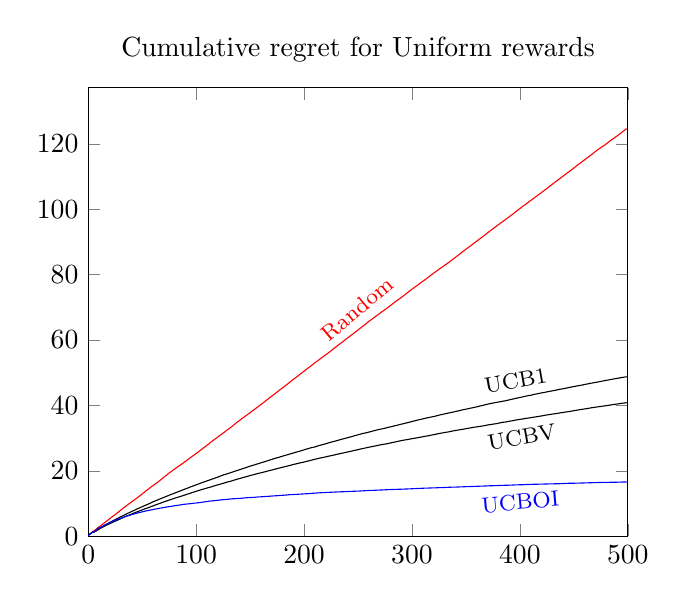
\begin{tikzpicture}
	\begin{axis}[
		title={Cumulative regret for Uniform rewards},
		%xlabel={Total number of pulls},
		xmin=0, xmax=500,
		ymin=0, %ymax=20,
	%	ymajorgrids=true,
		grid style=dashed
	]
	\addplot[red] coordinates {
(0,0.28001888247)(1,0.530072426181)(2,0.756919527015)(3,1.00466274313)(4,1.27259808436)(5,1.52447028995)(6,1.80813529604)(7,2.06233082172)(8,2.29240219926)(9,2.55774358946)(10,2.85583495655)(11,3.08188879654)(12,3.31289443813)(13,3.57451537822)(14,3.83117012762)(15,4.10775474676)(16,4.35424508853)(17,4.59599892876)(18,4.87101538254)(19,5.095674736)(20,5.38896865728)(21,5.64800403981)(22,5.86177121612)(23,6.12143456581)(24,6.37370497797)(25,6.62106349737)(26,6.85092696143)(27,7.13566082042)(28,7.37828131645)(29,7.63874723675)(30,7.92898927757)(31,8.19823318018)(32,8.45216785404)(33,8.71969748)(34,8.9511254445)(35,9.20535374354)(36,9.42916807952)(37,9.71231589696)(38,9.9632489543)(39,10.1866932034)(40,10.431706531)(41,10.6734331454)(42,10.9422589447)(43,11.1661045502)(44,11.3986736784)(45,11.6298305195)(46,11.8885185027)(47,12.1416125709)(48,12.3899886246)(49,12.6469504889)(50,12.9294403293)(51,13.2148980965)(52,13.4438587641)(53,13.689083812)(54,13.9695145325)(55,14.2208141563)(56,14.4587494683)(57,14.7168091169)(58,14.9829376675)(59,15.2423263674)(60,15.4665465216)(61,15.7162403255)(62,15.9486153245)(63,16.1988313582)(64,16.4289668224)(65,16.6717242624)(66,16.9400749899)(67,17.1909703837)(68,17.4547577431)(69,17.7229697269)(70,18.0070358193)(71,18.2748537976)(72,18.5317744398)(73,18.7833355888)(74,19.0488874075)(75,19.3479392957)(76,19.5586457862)(77,19.7965247562)(78,20.0328854153)(79,20.3104445009)(80,20.5382525777)(81,20.7641292205)(82,21.0189843863)(83,21.2357933876)(84,21.4555906503)(85,21.6735359831)(86,21.9200705188)(87,22.1326218479)(88,22.3724478913)(89,22.6162178878)(90,22.869858161)(91,23.1087183003)(92,23.3581433067)(93,23.6098485899)(94,23.8651777048)(95,24.1164850094)(96,24.3427313856)(97,24.5817824217)(98,24.810172178)(99,25.0670066748)(100,25.2825777152)(101,25.5302492086)(102,25.7804281328)(103,26.0297924367)(104,26.2993502488)(105,26.5446859632)(106,26.7732961266)(107,27.0405702243)(108,27.2929570809)(109,27.5463182595)(110,27.8114184821)(111,28.0575914788)(112,28.283648755)(113,28.5831586597)(114,28.8316651564)(115,29.0893973879)(116,29.3545768225)(117,29.5908408273)(118,29.8339816234)(119,30.0633025578)(120,30.3259310082)(121,30.5875772535)(122,30.8333378214)(123,31.0589385676)(124,31.2972351647)(125,31.5323057034)(126,31.7643199612)(127,32.0183000521)(128,32.3050529051)(129,32.5357276971)(130,32.7850779056)(131,33.0204265517)(132,33.2671416199)(133,33.5084191752)(134,33.7896868592)(135,34.0426791864)(136,34.3214068528)(137,34.6061144431)(138,34.8572033298)(139,35.1224244887)(140,35.3534529613)(141,35.6058036371)(142,35.866714348)(143,36.1234188421)(144,36.3479326625)(145,36.5793166273)(146,36.8081220577)(147,37.0707458067)(148,37.3159063461)(149,37.5405052149)(150,37.7806737672)(151,38.0539772717)(152,38.3195444171)(153,38.5374306231)(154,38.7693909194)(155,39.0130613879)(156,39.2765213111)(157,39.5054245817)(158,39.7635091389)(159,40.0411413746)(160,40.3024984054)(161,40.5381765798)(162,40.7851131626)(163,41.031583447)(164,41.2819179314)(165,41.5586068715)(166,41.8058497613)(167,42.0456004355)(168,42.3338523884)(169,42.5987889118)(170,42.8232869889)(171,43.077167989)(172,43.3212898902)(173,43.5694453813)(174,43.8583089968)(175,44.1018042771)(176,44.3379448533)(177,44.6157626994)(178,44.8608721077)(179,45.117784675)(180,45.3534959403)(181,45.607253687)(182,45.8589339689)(183,46.1148774625)(184,46.3717464388)(185,46.6281775613)(186,46.9205630373)(187,47.1763864358)(188,47.453288412)(189,47.7157243678)(190,47.9464014217)(191,48.2055227236)(192,48.449988599)(193,48.673423084)(194,48.9320733418)(195,49.1858475476)(196,49.4799757345)(197,49.740632432)(198,49.981738621)(199,50.2268753057)(200,50.4921305217)(201,50.722898884)(202,50.9876315752)(203,51.2475845061)(204,51.5178952752)(205,51.7656142171)(206,52.0138899208)(207,52.2487586574)(208,52.5151438834)(209,52.7911886654)(210,53.0516333471)(211,53.2855681688)(212,53.498232851)(213,53.7269199519)(214,53.9928672513)(215,54.255627027)(216,54.5182140423)(217,54.7449126891)(218,54.9937654752)(219,55.2245813721)(220,55.4406958275)(221,55.695307345)(222,55.9362396316)(223,56.208149942)(224,56.4555068505)(225,56.7222204048)(226,56.9990088705)(227,57.2649308728)(228,57.4915214446)(229,57.7695779354)(230,58.0137130415)(231,58.2761354053)(232,58.5367376159)(233,58.7827315624)(234,59.0078800006)(235,59.2707225437)(236,59.5237742622)(237,59.7719750855)(238,60.0642548068)(239,60.2926732771)(240,60.5555885796)(241,60.8194182993)(242,61.0449300912)(243,61.3204822765)(244,61.5579199601)(245,61.806254694)(246,62.0637994587)(247,62.3424228133)(248,62.580852934)(249,62.8332825321)(250,63.0946190428)(251,63.3616599931)(252,63.6168311219)(253,63.8665722725)(254,64.1173965442)(255,64.3432279615)(256,64.6099802757)(257,64.8786811761)(258,65.1537190117)(259,65.4455289842)(260,65.6976500815)(261,65.9507945809)(262,66.1551952744)(263,66.4108308607)(264,66.6551966083)(265,66.8945961472)(266,67.1334150565)(267,67.4031858439)(268,67.6595666108)(269,67.8548224464)(270,68.1202214964)(271,68.3771823863)(272,68.6301806404)(273,68.8537060545)(274,69.0961691545)(275,69.3089807148)(276,69.551206613)(277,69.7990579618)(278,70.04214883)(279,70.2997818334)(280,70.5712508735)(281,70.8099071343)(282,71.0761510342)(283,71.33035679)(284,71.5765092431)(285,71.8366442625)(286,72.0793298955)(287,72.319396842)(288,72.5226983278)(289,72.7849391434)(290,73.004931532)(291,73.2545180823)(292,73.5086031521)(293,73.7818770041)(294,74.0480983898)(295,74.2948719549)(296,74.5495509534)(297,74.8160508573)(298,75.0737576259)(299,75.3097143138)(300,75.5703296433)(301,75.7974364357)(302,76.0366014586)(303,76.2686073638)(304,76.5080034976)(305,76.7491491081)(306,76.9920220459)(307,77.2412863021)(308,77.5065015941)(309,77.7454752097)(310,77.9781509668)(311,78.2132990589)(312,78.4497297085)(313,78.6949381525)(314,78.9290924075)(315,79.2212945078)(316,79.4370639996)(317,79.7111122612)(318,79.9684099382)(319,80.2040251316)(320,80.4497737825)(321,80.6901246878)(322,80.9232378844)(323,81.1508421165)(324,81.4293531555)(325,81.6528244282)(326,81.909360653)(327,82.0999243604)(328,82.3187801846)(329,82.5579449136)(330,82.7831951732)(331,83.0325443158)(332,83.2747164942)(333,83.5226886851)(334,83.7403368664)(335,83.9924586956)(336,84.2362098552)(337,84.4921727499)(338,84.7380818355)(339,84.9663958217)(340,85.2433143)(341,85.5080627274)(342,85.7538565805)(343,86.0041528526)(344,86.2563760134)(345,86.5101822569)(346,86.7834971798)(347,87.0379750967)(348,87.2569115024)(349,87.5151503856)(350,87.796864502)(351,88.052294979)(352,88.2742102805)(353,88.5160567636)(354,88.7518650593)(355,89.0074651137)(356,89.2466179096)(357,89.5198169116)(358,89.7690059747)(359,90.0133658096)(360,90.2509509333)(361,90.5373137799)(362,90.7637034372)(363,91.0321030876)(364,91.2691370357)(365,91.4989196716)(366,91.7567785799)(367,92.0095657243)(368,92.2747200107)(369,92.5374908274)(370,92.7947212754)(371,93.0488742958)(372,93.302692217)(373,93.5366147436)(374,93.8033303178)(375,94.0551687833)(376,94.2873693581)(377,94.5353583888)(378,94.7900988715)(379,95.0229644081)(380,95.2724587565)(381,95.4950468139)(382,95.7548427561)(383,96.00806948)(384,96.2547521623)(385,96.4651186259)(386,96.725036859)(387,96.9620668217)(388,97.2112623877)(389,97.4326455769)(390,97.6802555398)(391,97.9556048348)(392,98.2112111941)(393,98.433269452)(394,98.6853070557)(395,98.9799654682)(396,99.233032123)(397,99.4935940692)(398,99.7341321762)(399,100.003778334)(400,100.248506382)(401,100.492261371)(402,100.749683452)(403,101.009752031)(404,101.230277136)(405,101.446483319)(406,101.704991883)(407,101.974185368)(408,102.230896794)(409,102.455049577)(410,102.683676166)(411,102.916035283)(412,103.178744048)(413,103.413479692)(414,103.668247141)(415,103.921964593)(416,104.174295646)(417,104.41495045)(418,104.653289044)(419,104.885861666)(420,105.143362167)(421,105.39959709)(422,105.634982568)(423,105.894079167)(424,106.113791488)(425,106.374989137)(426,106.64531838)(427,106.910313592)(428,107.148140834)(429,107.404321963)(430,107.665582272)(431,107.92410245)(432,108.148996406)(433,108.42348733)(434,108.651321394)(435,108.898561805)(436,109.152674207)(437,109.405903545)(438,109.67230555)(439,109.897904615)(440,110.145438997)(441,110.410054362)(442,110.661790284)(443,110.906093009)(444,111.179809877)(445,111.401958874)(446,111.648755077)(447,111.872606207)(448,112.122949162)(449,112.383543608)(450,112.637436057)(451,112.903745123)(452,113.161585761)(453,113.425724999)(454,113.680620929)(455,113.942054777)(456,114.165135108)(457,114.428355522)(458,114.6595532)(459,114.909201216)(460,115.187383854)(461,115.418739673)(462,115.66742931)(463,115.90305295)(464,116.167415813)(465,116.423588189)(466,116.66230713)(467,116.917396931)(468,117.178149378)(469,117.4373585)(470,117.683262127)(471,117.94578194)(472,118.186711519)(473,118.451151223)(474,118.662597211)(475,118.875012467)(476,119.111482132)(477,119.32230072)(478,119.536258341)(479,119.768016322)(480,120.027601322)(481,120.270478006)(482,120.532187073)(483,120.784889912)(484,121.038136442)(485,121.270909913)(486,121.492800014)(487,121.73772082)(488,121.973288497)(489,122.196617196)(490,122.444152929)(491,122.699965351)(492,122.963977674)(493,123.198855487)(494,123.434219341)(495,123.696594173)(496,123.954039556)(497,124.19484158)(498,124.466005803)(499,124.687093406)
		}node[pos=0.52](endofplotsquare){} ;
		\node [red,above,rotate=40] at (endofplotsquare) {\footnotesize Random};
	\addplot[black] coordinates {
(0,0.23806751075)(1,0.504032121251)(2,0.749438686685)(3,0.982369494976)(4,1.22701825532)(5,1.2448211963)(6,1.41064367973)(7,1.65517563642)(8,1.92359499134)(9,2.28951207956)(10,2.45065487607)(11,2.5828548811)(12,2.73021142278)(13,2.90953239397)(14,3.06762414828)(15,3.2677447944)(16,3.4599551207)(17,3.6370524296)(18,3.8474648816)(19,4.0170315656)(20,4.21750115022)(21,4.38168637863)(22,4.55498553756)(23,4.73567398248)(24,4.90662692205)(25,5.0476280791)(26,5.21937211129)(27,5.40975880233)(28,5.58053746968)(29,5.74685242768)(30,5.9278698946)(31,6.0766413139)(32,6.2481870805)(33,6.39325159594)(34,6.5706799554)(35,6.72067531612)(36,6.88897492887)(37,7.04451993303)(38,7.1938424298)(39,7.33305549167)(40,7.50451481273)(41,7.66287582591)(42,7.79924376857)(43,7.95373324698)(44,8.11343549334)(45,8.29191739767)(46,8.4481647071)(47,8.57689790747)(48,8.7058321734)(49,8.87289439844)(50,9.01992047095)(51,9.18735801542)(52,9.31676781314)(53,9.44613152845)(54,9.59998149595)(55,9.7285349725)(56,9.88128617077)(57,10.0242117733)(58,10.1956715001)(59,10.353224232)(60,10.4996962385)(61,10.6626871291)(62,10.7777430443)(63,10.9251271352)(64,11.0553269945)(65,11.1785042932)(66,11.3258631522)(67,11.4601681347)(68,11.5870818436)(69,11.7242032213)(70,11.8486654857)(71,11.9678033029)(72,12.1250172613)(73,12.2467607036)(74,12.394639864)(75,12.5243874552)(76,12.6757510685)(77,12.7969697107)(78,12.8904441121)(79,13.0341926315)(80,13.1669785277)(81,13.285502447)(82,13.4333798634)(83,13.5656283453)(84,13.6961787499)(85,13.8090748871)(86,13.9508679596)(87,14.0678843892)(88,14.1830609974)(89,14.3286130171)(90,14.4536466982)(91,14.5760687369)(92,14.7175621867)(93,14.8132116513)(94,14.965830781)(95,15.1044759592)(96,15.2200063986)(97,15.3416779055)(98,15.4611040267)(99,15.5796113666)(100,15.7161614317)(101,15.8262998211)(102,15.9521135061)(103,16.0631443606)(104,16.2060684199)(105,16.3198063266)(106,16.4418294916)(107,16.557402137)(108,16.6810796107)(109,16.7876642644)(110,16.9062780183)(111,17.0301381307)(112,17.1384049289)(113,17.2581741136)(114,17.3602873695)(115,17.4967206069)(116,17.6084943517)(117,17.7103154026)(118,17.8345543332)(119,17.943409854)(120,18.0598799556)(121,18.1967344912)(122,18.3332909951)(123,18.4441062051)(124,18.5685966966)(125,18.7036921304)(126,18.8173471301)(127,18.9067333748)(128,19.0039278542)(129,19.1029486221)(130,19.2149365918)(131,19.3417563001)(132,19.4452539829)(133,19.5466650573)(134,19.662930119)(135,19.7711268146)(136,19.8672411671)(137,19.9984570727)(138,20.1020677035)(139,20.2007270389)(140,20.316092699)(141,20.4120190339)(142,20.5279366757)(143,20.6585189818)(144,20.7618501405)(145,20.8572521397)(146,20.9587613005)(147,21.0878726893)(148,21.208732887)(149,21.3194923699)(150,21.4085149997)(151,21.5272066869)(152,21.6242794518)(153,21.7157814569)(154,21.8137369429)(155,21.9422068326)(156,22.0277521136)(157,22.1312920806)(158,22.2213694118)(159,22.3448248897)(160,22.4331840577)(161,22.5452780434)(162,22.6390370413)(163,22.7292264474)(164,22.8364384108)(165,22.9405439997)(166,23.0454323457)(167,23.1732282872)(168,23.2736270602)(169,23.3800427959)(170,23.4736321318)(171,23.5927152827)(172,23.7052866091)(173,23.8068192873)(174,23.8998493029)(175,23.982420926)(176,24.0868494287)(177,24.1636949006)(178,24.279939731)(179,24.365795611)(180,24.4690237135)(181,24.5922965139)(182,24.6917359845)(183,24.7743901047)(184,24.8547044845)(185,24.952090193)(186,25.0550412812)(187,25.1529970535)(188,25.2512901034)(189,25.3515447174)(190,25.4361210387)(191,25.5395174842)(192,25.6320000085)(193,25.7386245688)(194,25.8206212649)(195,25.9259193871)(196,26.0081531498)(197,26.1101829268)(198,26.2240259099)(199,26.3225019994)(200,26.4146802311)(201,26.5162218659)(202,26.6293223897)(203,26.7250494501)(204,26.8107258428)(205,26.9006311178)(206,27.0136428013)(207,27.1062371001)(208,27.1699755729)(209,27.2352160537)(210,27.3038266499)(211,27.4005103551)(212,27.5401452951)(213,27.6328998637)(214,27.7321757375)(215,27.8102756234)(216,27.9136626467)(217,28.0183455838)(218,28.0907318537)(219,28.1727595929)(220,28.2785626676)(221,28.3564238187)(222,28.4737943337)(223,28.572426772)(224,28.6824876628)(225,28.7590600838)(226,28.8545116365)(227,28.9290685183)(228,29.0287772495)(229,29.0958157004)(230,29.1998003807)(231,29.295584291)(232,29.3814272387)(233,29.4869426102)(234,29.5907551877)(235,29.6705511958)(236,29.7400738085)(237,29.8490199292)(238,29.9321318953)(239,29.9994810011)(240,30.0942281774)(241,30.2029292415)(242,30.2782163054)(243,30.3707225572)(244,30.4527604755)(245,30.5553491832)(246,30.6574055603)(247,30.7615731606)(248,30.8518645731)(249,30.930585083)(250,31.0096486851)(251,31.1223079148)(252,31.2012165282)(253,31.2905934513)(254,31.3910349049)(255,31.4539933827)(256,31.520852575)(257,31.5951606983)(258,31.6749780487)(259,31.7464225947)(260,31.8420683403)(261,31.9307371101)(262,31.9927508805)(263,32.0937680308)(264,32.1965696012)(265,32.2614749003)(266,32.3550692544)(267,32.4470168038)(268,32.5287227998)(269,32.6089907436)(270,32.6722380739)(271,32.7561308173)(272,32.8173132181)(273,32.8809689578)(274,32.9693507946)(275,33.0433149165)(276,33.1147443619)(277,33.2219829874)(278,33.296509009)(279,33.3793198105)(280,33.4484855897)(281,33.5203043255)(282,33.6060166762)(283,33.6825244676)(284,33.7688802021)(285,33.8364045952)(286,33.9125290021)(287,34.0032698942)(288,34.1117780792)(289,34.1842850071)(290,34.2640988603)(291,34.3383710952)(292,34.421643418)(293,34.4930426132)(294,34.6020129136)(295,34.6599150171)(296,34.7360907321)(297,34.8198541207)(298,34.904889102)(299,35.0048346571)(300,35.0973950166)(301,35.1677949476)(302,35.2437590185)(303,35.3376049642)(304,35.4328860075)(305,35.5051625644)(306,35.6012058081)(307,35.6631109728)(308,35.7303099977)(309,35.8032745922)(310,35.8834430467)(311,35.9710368011)(312,36.0482545451)(313,36.1182922136)(314,36.1960059615)(315,36.26696678)(316,36.3368128846)(317,36.3981927459)(318,36.4688554682)(319,36.536099612)(320,36.5896011036)(321,36.6771701132)(322,36.7624940689)(323,36.8509431773)(324,36.9397787959)(325,37.0275581243)(326,37.1067974857)(327,37.1657140295)(328,37.2412456335)(329,37.3143910381)(330,37.4004374749)(331,37.4589271731)(332,37.5481430375)(333,37.6055003391)(334,37.6858921405)(335,37.7592106104)(336,37.8456791835)(337,37.9143845657)(338,37.9583008965)(339,38.022039602)(340,38.1376517879)(341,38.2033563811)(342,38.2667544646)(343,38.3314154765)(344,38.415699191)(345,38.499638056)(346,38.5925254803)(347,38.6483330203)(348,38.738170757)(349,38.7897204281)(350,38.8543506242)(351,38.9268686569)(352,38.9917740477)(353,39.0689120793)(354,39.151098038)(355,39.2184366237)(356,39.2743603266)(357,39.3611915157)(358,39.4280473618)(359,39.4951182876)(360,39.575098096)(361,39.6575405235)(362,39.7452384667)(363,39.8316884612)(364,39.9024790181)(365,39.9739938455)(366,40.0465965537)(367,40.1362891243)(368,40.2280391699)(369,40.3079145715)(370,40.3751647579)(371,40.4535888551)(372,40.5292608817)(373,40.5885853974)(374,40.6676407197)(375,40.7256255629)(376,40.7895651777)(377,40.854188815)(378,40.9298501654)(379,40.9765345529)(380,41.0366699485)(381,41.1067095588)(382,41.1579720179)(383,41.2137514483)(384,41.2755098957)(385,41.3410062781)(386,41.3931322937)(387,41.473765261)(388,41.5467558458)(389,41.6111630243)(390,41.7055609423)(391,41.7678058321)(392,41.8520401696)(393,41.9159468843)(394,41.9973474654)(395,42.0917770877)(396,42.1662915086)(397,42.2310746643)(398,42.2879276672)(399,42.3729781053)(400,42.4358679889)(401,42.4885613025)(402,42.5819717264)(403,42.6550808077)(404,42.744059702)(405,42.810637459)(406,42.8694822389)(407,42.9369850637)(408,43.0051913897)(409,43.0603198058)(410,43.1152435276)(411,43.1843901784)(412,43.2816479638)(413,43.3659261791)(414,43.4380392393)(415,43.4986914364)(416,43.559982371)(417,43.636415227)(418,43.68613588)(419,43.7652425315)(420,43.8406081789)(421,43.8843088357)(422,43.9521944256)(423,44.0143540942)(424,44.0789840231)(425,44.1476469845)(426,44.2251640582)(427,44.2893954787)(428,44.3475639503)(429,44.403302822)(430,44.4557922344)(431,44.5323610244)(432,44.5929935222)(433,44.6503060329)(434,44.7302628225)(435,44.7967519734)(436,44.867677122)(437,44.9442601568)(438,44.997848392)(439,45.0478341007)(440,45.1088414509)(441,45.1685497313)(442,45.2200617426)(443,45.3089585823)(444,45.3785240175)(445,45.4618792724)(446,45.5305727714)(447,45.5861485913)(448,45.6545536348)(449,45.7203871832)(450,45.7784500534)(451,45.8282652217)(452,45.9070156115)(453,45.967835086)(454,46.0366720962)(455,46.0828707191)(456,46.1507566913)(457,46.1969189593)(458,46.2548761532)(459,46.3392942213)(460,46.409103316)(461,46.4685272888)(462,46.5483551321)(463,46.6034606397)(464,46.6850447031)(465,46.7488201913)(466,46.8069768002)(467,46.8584677174)(468,46.9243257154)(469,46.9917950578)(470,47.041826854)(471,47.0955155339)(472,47.1599564826)(473,47.2216596289)(474,47.2904249127)(475,47.3547604156)(476,47.4195222351)(477,47.4885606108)(478,47.5601586027)(479,47.6205443826)(480,47.6733588528)(481,47.742276551)(482,47.8016690911)(483,47.860174351)(484,47.9364177771)(485,47.9904767146)(486,48.0373235906)(487,48.1180830961)(488,48.1562318442)(489,48.2152000743)(490,48.2736335234)(491,48.3306318916)(492,48.3956991475)(493,48.4661378541)(494,48.5112880224)(495,48.5718347177)(496,48.6198443619)(497,48.6842508566)(498,48.7284440596)(499,48.7840448577)
		}node[pos=0.8](endofplotsquare){} ;
		\node [black,above,rotate=10] at (endofplotsquare) {\footnotesize UCB1};
	\addplot[black] coordinates {
(0,0.256926421523)(1,0.501030958967)(2,0.740664127156)(3,0.991393550012)(4,1.20886870841)(5,1.23350524216)(6,1.35280034028)(7,1.50953948514)(8,1.71487168247)(9,1.9111440821)(10,2.13992098946)(11,2.32412210225)(12,2.50913307203)(13,2.67454581554)(14,2.86339176604)(15,3.04094704252)(16,3.20818387734)(17,3.39095263205)(18,3.53570509594)(19,3.68307043066)(20,3.82991388574)(21,3.97297980834)(22,4.12167863649)(23,4.28066760974)(24,4.44220280639)(25,4.60061670242)(26,4.72940952879)(27,4.86303572354)(28,5.02589724051)(29,5.17089705189)(30,5.32617568099)(31,5.47407730446)(32,5.61896932259)(33,5.77248980922)(34,5.93637647348)(35,6.09043283565)(36,6.22169137772)(37,6.34980655146)(38,6.47302136305)(39,6.61253517984)(40,6.71991687454)(41,6.89780597143)(42,7.03086886013)(43,7.16684766992)(44,7.28702559319)(45,7.40685177667)(46,7.52963804937)(47,7.66629688693)(48,7.79760139963)(49,7.91807651572)(50,8.03185584087)(51,8.17396930057)(52,8.31161356028)(53,8.42080810004)(54,8.53387954856)(55,8.64106366241)(56,8.76842222643)(57,8.89027287207)(58,9.00246011587)(59,9.13471175779)(60,9.2573406646)(61,9.395278008)(62,9.52304028794)(63,9.63355418695)(64,9.74954955767)(65,9.87066958655)(66,9.99305574686)(67,10.1216776429)(68,10.2340980261)(69,10.3439304558)(70,10.4765402523)(71,10.587825793)(72,10.6957801161)(73,10.8174364824)(74,10.9188608906)(75,11.0417334491)(76,11.1423422573)(77,11.24654753)(78,11.3801619973)(79,11.4992713423)(80,11.6088468992)(81,11.7071747973)(82,11.8179123776)(83,11.9082002416)(84,12.0255483075)(85,12.1051751515)(86,12.2112831589)(87,12.3266137002)(88,12.4197327437)(89,12.5327432957)(90,12.6325113631)(91,12.7704704827)(92,12.8847837678)(93,12.9638292468)(94,13.0658628985)(95,13.1845065784)(96,13.3087214389)(97,13.4016930672)(98,13.5210949638)(99,13.6196986728)(100,13.7203169007)(101,13.8255952033)(102,13.9379073958)(103,14.0339601195)(104,14.1285540053)(105,14.238657989)(106,14.3299406141)(107,14.444435887)(108,14.5199075419)(109,14.6241236045)(110,14.7303184273)(111,14.8247068102)(112,14.9158601499)(113,14.9969302252)(114,15.0932805661)(115,15.1894195758)(116,15.3068904529)(117,15.3971962228)(118,15.5164766887)(119,15.6136828632)(120,15.7053958847)(121,15.7794549747)(122,15.8884072992)(123,15.977111818)(124,16.0855284635)(125,16.183893584)(126,16.2628190292)(127,16.3707613129)(128,16.4798487761)(129,16.5718472679)(130,16.6574117671)(131,16.7331794871)(132,16.8134249728)(133,16.9115509848)(134,17.0191765223)(135,17.1343618084)(136,17.2253022047)(137,17.3189632298)(138,17.4343109297)(139,17.52849486)(140,17.6214015108)(141,17.7036531321)(142,17.7987539686)(143,17.8921251081)(144,17.9812117859)(145,18.0697269142)(146,18.1411349608)(147,18.2442739284)(148,18.3627172446)(149,18.4479053088)(150,18.5440884737)(151,18.6394062918)(152,18.7095439677)(153,18.7863642195)(154,18.8837734982)(155,18.9704704143)(156,19.050295266)(157,19.156398655)(158,19.241214994)(159,19.3330834294)(160,19.392168028)(161,19.4721391951)(162,19.5527925101)(163,19.6336631665)(164,19.7173084987)(165,19.8124109929)(166,19.9050606558)(167,19.9828815539)(168,20.0649769952)(169,20.157686966)(170,20.2309538467)(171,20.3120550905)(172,20.4163518178)(173,20.4881280699)(174,20.5755994583)(175,20.6721467218)(176,20.7600464195)(177,20.8289726778)(178,20.9198955817)(179,21.0060224683)(180,21.0870076935)(181,21.1559356079)(182,21.2364021264)(183,21.3336782633)(184,21.4129671222)(185,21.4910646523)(186,21.5808604258)(187,21.6585587325)(188,21.752591122)(189,21.8338411431)(190,21.9407879623)(191,22.0099651886)(192,22.0790669047)(193,22.1624963974)(194,22.2408336434)(195,22.3290532177)(196,22.4067462073)(197,22.4678487969)(198,22.5356874872)(199,22.5995962394)(200,22.6820630998)(201,22.7584227418)(202,22.855229115)(203,22.9313120343)(204,23.0144611783)(205,23.1029016924)(206,23.1868731416)(207,23.2731814142)(208,23.3633195449)(209,23.4429446567)(210,23.5272238466)(211,23.6114753332)(212,23.6687562936)(213,23.7586145346)(214,23.8544918167)(215,23.9204560593)(216,23.9851620011)(217,24.0409240835)(218,24.1205505141)(219,24.1868834145)(220,24.2630256252)(221,24.3300274915)(222,24.4298442156)(223,24.5014986688)(224,24.5631623649)(225,24.6246299665)(226,24.6966256172)(227,24.7746611902)(228,24.8430181567)(229,24.9230555368)(230,25.0138244706)(231,25.0898314601)(232,25.1680750261)(233,25.2331091117)(234,25.3140053981)(235,25.3801039427)(236,25.4374206116)(237,25.5188042812)(238,25.6011278444)(239,25.6659043382)(240,25.7367121633)(241,25.8004279118)(242,25.8771122194)(243,25.9431270853)(244,26.017392106)(245,26.1123929622)(246,26.2125426194)(247,26.2613994777)(248,26.3319239231)(249,26.392406284)(250,26.4670429364)(251,26.5571568667)(252,26.6401844959)(253,26.7211565523)(254,26.7953324561)(255,26.8579278701)(256,26.9357000351)(257,26.9907632952)(258,27.0789009087)(259,27.1524312174)(260,27.2058148777)(261,27.2821648426)(262,27.357152837)(263,27.4234714362)(264,27.4700458344)(265,27.5405142551)(266,27.6091822859)(267,27.6858129263)(268,27.7302376965)(269,27.821286172)(270,27.8877264443)(271,27.9566457155)(272,28.0118958578)(273,28.0686188981)(274,28.1256194071)(275,28.1845475084)(276,28.2346035994)(277,28.3043736278)(278,28.3498773496)(279,28.4289060737)(280,28.5208207899)(281,28.5890409327)(282,28.657286234)(283,28.7298858403)(284,28.8004937583)(285,28.8539699686)(286,28.9512443249)(287,29.0150206056)(288,29.0941936177)(289,29.1636071381)(290,29.2435105425)(291,29.2998741184)(292,29.3472131315)(293,29.4222739236)(294,29.4745078052)(295,29.5191517022)(296,29.5725143416)(297,29.6222948995)(298,29.7128751738)(299,29.7740245442)(300,29.8311679164)(301,29.8838869919)(302,29.9412027779)(303,29.9915758842)(304,30.0536036336)(305,30.108382261)(306,30.1705290859)(307,30.2312335685)(308,30.2845477354)(309,30.3751099109)(310,30.4209813759)(311,30.4949213228)(312,30.5512075344)(313,30.6107608252)(314,30.6564622104)(315,30.7226163394)(316,30.7833981295)(317,30.8612903309)(318,30.9300702483)(319,30.9942355927)(320,31.0574746576)(321,31.1071257419)(322,31.1840067677)(323,31.2471175359)(324,31.3329985325)(325,31.4044830951)(326,31.4566632639)(327,31.5060888471)(328,31.5928225181)(329,31.6390198715)(330,31.6991334978)(331,31.7545147441)(332,31.8154389617)(333,31.8620422954)(334,31.9229689902)(335,31.9914054353)(336,32.0664954727)(337,32.134308799)(338,32.204890139)(339,32.2629200626)(340,32.3242094801)(341,32.3734083805)(342,32.4406539761)(343,32.4854990058)(344,32.5561076022)(345,32.6104167492)(346,32.6640799712)(347,32.7064739225)(348,32.764343935)(349,32.8281536656)(350,32.8897757731)(351,32.9524818014)(352,33.0139308167)(353,33.0764392173)(354,33.1259132982)(355,33.1669459755)(356,33.2451591063)(357,33.3051297359)(358,33.3522031109)(359,33.3941235)(360,33.4467890379)(361,33.4987191955)(362,33.5471598338)(363,33.6007870231)(364,33.6497921039)(365,33.6940145316)(366,33.7460699671)(367,33.8150894528)(368,33.8859518008)(369,33.9424287117)(370,34.0023879324)(371,34.0714134157)(372,34.1165692246)(373,34.1720458433)(374,34.2226612461)(375,34.2698395442)(376,34.3320570272)(377,34.3718229355)(378,34.4159403271)(379,34.4868858638)(380,34.5513430867)(381,34.635305253)(382,34.7079092005)(383,34.7688191192)(384,34.8201655538)(385,34.8673695426)(386,34.905732006)(387,34.9530036183)(388,35.0063092642)(389,35.0833717998)(390,35.1444130099)(391,35.2079634649)(392,35.2647977778)(393,35.3139349714)(394,35.3850052295)(395,35.4548607525)(396,35.5251633142)(397,35.5825526244)(398,35.6392989259)(399,35.678613698)(400,35.7288215824)(401,35.7856471786)(402,35.8301524915)(403,35.8951727293)(404,35.9466123202)(405,36.0095929673)(406,36.0693327992)(407,36.1053376765)(408,36.149026258)(409,36.2004382628)(410,36.265981905)(411,36.3099281054)(412,36.3758710526)(413,36.4275937482)(414,36.4720633694)(415,36.521761173)(416,36.5827922329)(417,36.6264864997)(418,36.6863733147)(419,36.7446682001)(420,36.7875487484)(421,36.8516368839)(422,36.9250298315)(423,36.9943613774)(424,37.0461322211)(425,37.0962067686)(426,37.142228186)(427,37.186374362)(428,37.2560787424)(429,37.2987567252)(430,37.352504935)(431,37.3945653678)(432,37.4423221464)(433,37.4897416648)(434,37.547176119)(435,37.5943409529)(436,37.6488269495)(437,37.708971897)(438,37.7714843805)(439,37.813725758)(440,37.8579514489)(441,37.9186628358)(442,37.974906294)(443,38.011897281)(444,38.056705222)(445,38.0982616302)(446,38.1496165319)(447,38.2139637485)(448,38.2731251292)(449,38.3361589006)(450,38.3963350985)(451,38.4525539009)(452,38.5113343281)(453,38.575590038)(454,38.627492531)(455,38.6729395172)(456,38.719714317)(457,38.7781179289)(458,38.8332480537)(459,38.8849060363)(460,38.9417869652)(461,38.9830902691)(462,39.0337512967)(463,39.091479802)(464,39.1382076186)(465,39.2157181463)(466,39.2767109047)(467,39.3197459513)(468,39.3747500076)(469,39.4203073174)(470,39.4678621061)(471,39.5195087342)(472,39.5698010359)(473,39.6264839959)(474,39.6668125122)(475,39.7042238502)(476,39.7550861574)(477,39.8052201166)(478,39.8391266938)(479,39.8911697849)(480,39.9313551597)(481,39.9875811402)(482,40.0332901439)(483,40.0730074119)(484,40.1409638518)(485,40.1976524607)(486,40.2479779222)(487,40.307319951)(488,40.3447687844)(489,40.381849719)(490,40.444470102)(491,40.4823566044)(492,40.5357757523)(493,40.5860369378)(494,40.6374238176)(495,40.6818627263)(496,40.7124086607)(497,40.7569703245)(498,40.8077417535)(499,40.8562095169)
		}node[pos=0.8](endofplotsquare){} ;
		\node [black,below,rotate=10] at (endofplotsquare) {\footnotesize UCBV};
	\addplot[blue] coordinates {
(0,0.215760732893)(1,0.484450313718)(2,0.715967948291)(3,0.97649493256)(4,1.24102971372)(5,1.27476722556)(6,1.41973183111)(7,1.66680117642)(8,1.99072440149)(9,2.43726336683)(10,2.4978241793)(11,2.5971031916)(12,2.73013332049)(13,2.91939687602)(14,3.15651633958)(15,3.38162608568)(16,3.51598350458)(17,3.66085361272)(18,3.81842096525)(19,3.99122157667)(20,4.13240583974)(21,4.29155064953)(22,4.43138077549)(23,4.5874080293)(24,4.74741536126)(25,4.84472481992)(26,4.98152677129)(27,5.10167808374)(28,5.23319561141)(29,5.32544616556)(30,5.46772843089)(31,5.59410325873)(32,5.69712695603)(33,5.83038787047)(34,5.95253665065)(35,6.06036964322)(36,6.16739628166)(37,6.25444834734)(38,6.3612705048)(39,6.45228741848)(40,6.56444359132)(41,6.65685681682)(42,6.75831190166)(43,6.84916394466)(44,6.92580660064)(45,7.01767072022)(46,7.13755734783)(47,7.20447214196)(48,7.28797191605)(49,7.36531036186)(50,7.43890728038)(51,7.52236088653)(52,7.61586469648)(53,7.68975987079)(54,7.75506707478)(55,7.8231145379)(56,7.89860210279)(57,7.96456197682)(58,8.0028116545)(59,8.08337599961)(60,8.14872500598)(61,8.2159310569)(62,8.29526505263)(63,8.35115213487)(64,8.392208542)(65,8.46347221426)(66,8.531709687)(67,8.60262342689)(68,8.66140218675)(69,8.7104947204)(70,8.76713238232)(71,8.81889513788)(72,8.87376594933)(73,8.94664255463)(74,8.99334584731)(75,9.0320186091)(76,9.09117493048)(77,9.13896459185)(78,9.20544899114)(79,9.2798120443)(80,9.31349871334)(81,9.34503592333)(82,9.39220136705)(83,9.44771812064)(84,9.49200712308)(85,9.5485587002)(86,9.61259722064)(87,9.66639795037)(88,9.71427202634)(89,9.75036116283)(90,9.80158737834)(91,9.82113607676)(92,9.87707145555)(93,9.90094972027)(94,9.92933004556)(95,9.96770924699)(96,10.0034350104)(97,10.0495236364)(98,10.0913960651)(99,10.1163315921)(100,10.1388816762)(101,10.2005337287)(102,10.2324696507)(103,10.2687846358)(104,10.3167825164)(105,10.350895561)(106,10.4111820007)(107,10.4691808297)(108,10.5105235401)(109,10.5583386254)(110,10.5892127717)(111,10.6430527178)(112,10.7119315215)(113,10.746306879)(114,10.7759687972)(115,10.8129580627)(116,10.846815712)(117,10.8821130144)(118,10.9190927705)(119,10.9535234545)(120,10.9913650152)(121,11.0215022655)(122,11.0615537259)(123,11.0874378961)(124,11.1262747406)(125,11.1661516518)(126,11.1925566006)(127,11.2183231769)(128,11.2417772548)(129,11.2759175302)(130,11.3150631118)(131,11.3562645635)(132,11.3807544247)(133,11.4113766032)(134,11.4406515472)(135,11.459923635)(136,11.4868959472)(137,11.5079585083)(138,11.5339046943)(139,11.5571091095)(140,11.5677967449)(141,11.5784147122)(142,11.6036079648)(143,11.6390237713)(144,11.6863092401)(145,11.7138807111)(146,11.7411793265)(147,11.7697902881)(148,11.7846799531)(149,11.8107559181)(150,11.834406077)(151,11.8470817136)(152,11.8548648777)(153,11.8757281447)(154,11.8997847484)(155,11.9347528651)(156,11.9677027121)(157,11.9949130453)(158,12.0189643773)(159,12.0329261575)(160,12.0501319977)(161,12.0706363976)(162,12.1031152921)(163,12.1195087179)(164,12.1347150937)(165,12.1563574273)(166,12.1786638762)(167,12.2031457726)(168,12.2295298687)(169,12.2452092487)(170,12.2855938547)(171,12.3090461762)(172,12.3256446695)(173,12.3459496135)(174,12.3678465015)(175,12.390299881)(176,12.4182597192)(177,12.4353844183)(178,12.4811768324)(179,12.4915887679)(180,12.5156113511)(181,12.5297876591)(182,12.5547730515)(183,12.5914102721)(184,12.6048222241)(185,12.6428098389)(186,12.6817696569)(187,12.7005463579)(188,12.7102981448)(189,12.7313437322)(190,12.7411444735)(191,12.7676968157)(192,12.7915127825)(193,12.8017523923)(194,12.8126830263)(195,12.8470034918)(196,12.8673838069)(197,12.8845670122)(198,12.9083905381)(199,12.9215487221)(200,12.9400687989)(201,12.9582489788)(202,12.9775810758)(203,12.9936363474)(204,13.024835867)(205,13.0504877174)(206,13.0749337698)(207,13.1175142941)(208,13.1307901077)(209,13.1492498549)(210,13.1747135204)(211,13.2010506726)(212,13.2203578977)(213,13.2443546223)(214,13.2671212648)(215,13.287266282)(216,13.3068786459)(217,13.3228213325)(218,13.3396565195)(219,13.3515938414)(220,13.3793840133)(221,13.3929457028)(222,13.4107709607)(223,13.4228776629)(224,13.4322937109)(225,13.4441785244)(226,13.4625086032)(227,13.4856873509)(228,13.497470455)(229,13.5161256247)(230,13.5312042383)(231,13.5533537579)(232,13.56455678)(233,13.5706891726)(234,13.5820889385)(235,13.5900458194)(236,13.6040116485)(237,13.6199873717)(238,13.6297045418)(239,13.6487401575)(240,13.6670456153)(241,13.6719980339)(242,13.6874710863)(243,13.7049578206)(244,13.7138019947)(245,13.7328491461)(246,13.7499234908)(247,13.7608120365)(248,13.7671005403)(249,13.783566412)(250,13.7920907229)(251,13.8072170955)(252,13.8204151083)(253,13.8446253156)(254,13.8570949252)(255,13.8851351661)(256,13.9138657442)(257,13.9347362976)(258,13.954372605)(259,13.9626035104)(260,13.9808093455)(261,13.9958530858)(262,14.0037481639)(263,14.0119742971)(264,14.022819155)(265,14.0382502573)(266,14.0507326128)(267,14.067662675)(268,14.0833830618)(269,14.0970728585)(270,14.1155370474)(271,14.12890222)(272,14.1395391967)(273,14.1526814167)(274,14.1724919404)(275,14.1861878954)(276,14.2125257094)(277,14.2205651058)(278,14.2366846169)(279,14.2488325853)(280,14.2681143318)(281,14.2765050708)(282,14.2885978942)(283,14.3045825593)(284,14.3176994158)(285,14.3203220901)(286,14.3352703853)(287,14.3455950315)(288,14.3551601862)(289,14.3660673892)(290,14.3732458909)(291,14.3852009718)(292,14.40121514)(293,14.4205333355)(294,14.4329173306)(295,14.4385768367)(296,14.4530463169)(297,14.4664781577)(298,14.485616951)(299,14.4936893957)(300,14.5125895127)(301,14.5327022013)(302,14.5610097437)(303,14.5699659747)(304,14.5955341798)(305,14.5998126725)(306,14.6142208096)(307,14.6294270569)(308,14.6376627064)(309,14.6547180347)(310,14.6644482339)(311,14.6836628511)(312,14.7020044174)(313,14.7102557054)(314,14.7147051021)(315,14.7214720152)(316,14.7413820583)(317,14.7491053052)(318,14.7599386135)(319,14.7722130695)(320,14.7776274329)(321,14.7805747432)(322,14.7944231459)(323,14.8180532387)(324,14.8299122572)(325,14.8458551173)(326,14.8526604047)(327,14.8637322141)(328,14.8712691412)(329,14.8852495636)(330,14.8993270464)(331,14.9158314865)(332,14.9250832828)(333,14.943409726)(334,14.964516813)(335,14.9806462108)(336,14.9879426906)(337,14.9964638372)(338,15.0107466547)(339,15.0183078192)(340,15.0287893597)(341,15.0334395721)(342,15.0439260469)(343,15.0523780675)(344,15.0713299889)(345,15.085644675)(346,15.091040322)(347,15.1057088298)(348,15.1180575682)(349,15.1359845395)(350,15.1472886554)(351,15.1552131924)(352,15.1597247887)(353,15.1818517755)(354,15.1938514797)(355,15.2020682518)(356,15.2149496934)(357,15.2272000377)(358,15.2356010394)(359,15.2498795108)(360,15.2568486943)(361,15.2730196571)(362,15.2926873137)(363,15.3020661693)(364,15.3129535504)(365,15.3174315333)(366,15.3340948512)(367,15.344045525)(368,15.3619423475)(369,15.3683651542)(370,15.3911021976)(371,15.4087449462)(372,15.4271642534)(373,15.4320020848)(374,15.43778222)(375,15.4410829258)(376,15.4645419292)(377,15.4677996119)(378,15.4757580339)(379,15.4899620367)(380,15.5004248773)(381,15.5115373447)(382,15.5307027612)(383,15.5491088965)(384,15.5565489581)(385,15.5643650998)(386,15.578718415)(387,15.5821857276)(388,15.5916478459)(389,15.5971768048)(390,15.6085692556)(391,15.6217975557)(392,15.6421173949)(393,15.6464665366)(394,15.6587351291)(395,15.6771021357)(396,15.6884662492)(397,15.69612007)(398,15.7160222811)(399,15.7227239934)(400,15.7350387734)(401,15.7410683443)(402,15.7452529129)(403,15.7495274683)(404,15.7616283223)(405,15.7701046565)(406,15.7945323267)(407,15.8122044316)(408,15.829087557)(409,15.8341375489)(410,15.8429564181)(411,15.8641998533)(412,15.8737156868)(413,15.8874790529)(414,15.8924516703)(415,15.899367277)(416,15.9045924447)(417,15.9088348615)(418,15.9135045237)(419,15.9267066557)(420,15.9352510351)(421,15.9438606785)(422,15.9485203825)(423,15.961050406)(424,15.9666279956)(425,15.9724548843)(426,15.9824712166)(427,15.9920835107)(428,16.0041094071)(429,16.0138875851)(430,16.0226521967)(431,16.0272283447)(432,16.0293708988)(433,16.0344399726)(434,16.0418122925)(435,16.047020941)(436,16.0531540223)(437,16.0619386315)(438,16.0722973177)(439,16.0930848205)(440,16.1129860643)(441,16.1277669549)(442,16.1433304427)(443,16.1511413906)(444,16.171953243)(445,16.1834879504)(446,16.1906860968)(447,16.1967584952)(448,16.2035475107)(449,16.2076007245)(450,16.2103433301)(451,16.213887087)(452,16.2230048228)(453,16.2282949258)(454,16.2343178288)(455,16.246634781)(456,16.2537252791)(457,16.2661593697)(458,16.2726500622)(459,16.2799999173)(460,16.2924562308)(461,16.3045672026)(462,16.314263171)(463,16.3289588513)(464,16.336383052)(465,16.3438658257)(466,16.3543551773)(467,16.3658865976)(468,16.3708986035)(469,16.3768739227)(470,16.3853573533)(471,16.3952587045)(472,16.4110914489)(473,16.416526605)(474,16.4213767432)(475,16.4368195569)(476,16.4456004255)(477,16.4512954215)(478,16.4575918027)(479,16.4593705873)(480,16.4626039863)(481,16.4753842804)(482,16.4842219211)(483,16.4869209572)(484,16.4887424069)(485,16.4904282346)(486,16.4950011216)(487,16.5048104542)(488,16.5070240494)(489,16.5109901248)(490,16.517896789)(491,16.5294129375)(492,16.5511127333)(493,16.5575115206)(494,16.5623254822)(495,16.5685751358)(496,16.5755172773)(497,16.5855367133)(498,16.5930011841)(499,16.5985377119)
		}node[pos=0.8](endofplotsquare){} ;
		\node [blue,below, rotate=5] at (endofplotsquare) {\footnotesize UCBOI};
	\end{axis}
	\end{tikzpicture}

}\label{fig:1b}}%
\\
    \subfigure[]%
{\resizebox{0.5\linewidth}{!}{%triangular
	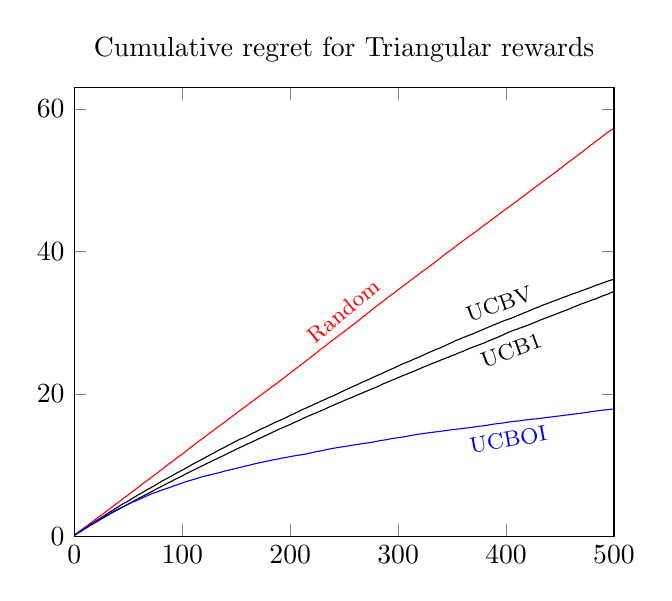
\begin{tikzpicture}
	\begin{axis}[
		title={Cumulative regret for Triangular rewards},
		%xlabel={Total number of pulls},
		xmin=0, xmax=500,
		ymin=0, %ymax=20,
	%	ymajorgrids=true,
		grid style=dashed
	]
	\addplot[red] coordinates {
(0,0.109940264536)(1,0.227747077839)(2,0.345619245586)(3,0.473631216458)(4,0.57865570476)(5,0.704984494099)(6,0.817777122795)(7,0.942727325463)(8,1.06144615695)(9,1.1713757287)(10,1.28623650636)(11,1.40296121016)(12,1.50620262327)(13,1.62116541491)(14,1.74183727291)(15,1.84434619927)(16,1.96343067349)(17,2.06690938456)(18,2.19092190835)(19,2.30519397493)(20,2.40953898434)(21,2.51813129409)(22,2.6416494138)(23,2.74088025081)(24,2.8557920194)(25,2.96079929829)(26,3.08858560032)(27,3.18952496258)(28,3.31736465516)(29,3.41717370489)(30,3.51586322596)(31,3.64314396141)(32,3.76151158844)(33,3.87096136477)(34,3.98177631245)(35,4.0907085224)(36,4.21674473701)(37,4.3392507648)(38,4.45532339872)(39,4.57003090932)(40,4.66694570931)(41,4.78197138481)(42,4.89577881831)(43,5.02184952989)(44,5.13612917935)(45,5.25253908298)(46,5.3653966304)(47,5.47959528173)(48,5.5915011197)(49,5.70477309944)(50,5.81849801315)(51,5.94459087948)(52,6.06070163996)(53,6.1683637612)(54,6.28869924632)(55,6.39727186887)(56,6.49792282745)(57,6.61883455462)(58,6.73320051523)(59,6.85640614468)(60,6.97322572021)(61,7.09082840773)(62,7.21696220211)(63,7.34304676017)(64,7.45022114386)(65,7.55901386726)(66,7.66695727212)(67,7.7684910565)(68,7.87095718015)(69,7.97612506621)(70,8.09394126966)(71,8.22270696059)(72,8.34714990926)(73,8.4615382213)(74,8.569973034)(75,8.67700223179)(76,8.79653663324)(77,8.91934396361)(78,9.02085349559)(79,9.14033043384)(80,9.24464319344)(81,9.35447289174)(82,9.47238397648)(83,9.61162627422)(84,9.72649607711)(85,9.85034192456)(86,9.97511079338)(87,10.086285602)(88,10.2052050468)(89,10.3080743946)(90,10.4254244759)(91,10.5364642955)(92,10.6490002109)(93,10.7568066693)(94,10.8731267252)(95,10.9866697201)(96,11.106188707)(97,11.2152192001)(98,11.3191181901)(99,11.4242941988)(100,11.5192602936)(101,11.6410358774)(102,11.7659370963)(103,11.8901070873)(104,12.0228405884)(105,12.1457582444)(106,12.2696191718)(107,12.3918355102)(108,12.4933381552)(109,12.6043360572)(110,12.719879152)(111,12.8456836282)(112,12.9720113475)(113,13.0941542436)(114,13.1982614655)(115,13.2968022002)(116,13.4065644749)(117,13.5210194315)(118,13.617860956)(119,13.733692168)(120,13.8650247694)(121,13.9665601489)(122,14.0790830238)(123,14.2122226725)(124,14.3262201005)(125,14.4434352217)(126,14.5440212715)(127,14.6613606247)(128,14.7585520861)(129,14.881511809)(130,15.0094830881)(131,15.119358596)(132,15.222936247)(133,15.318975868)(134,15.4308639863)(135,15.5481814174)(136,15.673150038)(137,15.7668905312)(138,15.8780685931)(139,15.9784976131)(140,16.0896582924)(141,16.2219793687)(142,16.3459256595)(143,16.4481176764)(144,16.5647892079)(145,16.676748063)(146,16.7942639604)(147,16.9201579268)(148,17.0285412912)(149,17.1392430169)(150,17.2630373258)(151,17.3670592156)(152,17.4892779716)(153,17.6178439528)(154,17.7098265679)(155,17.819268525)(156,17.9368228725)(157,18.039457)(158,18.1502972941)(159,18.2546082005)(160,18.3741398624)(161,18.4927376563)(162,18.6096194915)(163,18.7432180867)(164,18.8521567494)(165,18.9563237835)(166,19.0707513708)(167,19.176165651)(168,19.277387881)(169,19.3935843816)(170,19.5126778237)(171,19.6286168068)(172,19.7431070493)(173,19.8546740463)(174,19.9682274565)(175,20.0729723682)(176,20.1826884544)(177,20.3007379867)(178,20.4167345956)(179,20.5302471004)(180,20.6444823509)(181,20.758182792)(182,20.8541316462)(183,20.9809672508)(184,21.07781217)(185,21.1913538054)(186,21.2983382493)(187,21.4117151728)(188,21.5362247568)(189,21.6436636746)(190,21.7563780332)(191,21.879292177)(192,21.9865604844)(193,22.1157353689)(194,22.2191042413)(195,22.3414547592)(196,22.4546908981)(197,22.5693930108)(198,22.6969149251)(199,22.8149803711)(200,22.928421885)(201,23.0385488109)(202,23.1603815676)(203,23.2666748022)(204,23.3845157341)(205,23.4997763835)(206,23.6192652299)(207,23.7445697778)(208,23.8653373804)(209,23.9782923473)(210,24.0989651689)(211,24.1885689571)(212,24.3122185867)(213,24.4314397365)(214,24.5408809456)(215,24.6465490133)(216,24.780847627)(217,24.8952714185)(218,25.0137843546)(219,25.1282408758)(220,25.2469569469)(221,25.3455002539)(222,25.4813205171)(223,25.6171864519)(224,25.7247204421)(225,25.8517979955)(226,25.9649805248)(227,26.0922492842)(228,26.2193192613)(229,26.3388779339)(230,26.4424846994)(231,26.5547990811)(232,26.6683554798)(233,26.782386689)(234,26.9156124591)(235,27.0266465046)(236,27.1486459782)(237,27.279961033)(238,27.3952931576)(239,27.497769851)(240,27.6112806466)(241,27.730769063)(242,27.8337348719)(243,27.9458749766)(244,28.0664436666)(245,28.1901806824)(246,28.3031120868)(247,28.4252691151)(248,28.5377916382)(249,28.6443535604)(250,28.7531051986)(251,28.8663125873)(252,28.9749235323)(253,29.1025055878)(254,29.2196767389)(255,29.3348686303)(256,29.4503555006)(257,29.5615915864)(258,29.6654313337)(259,29.7721887208)(260,29.9003524148)(261,30.0141340521)(262,30.1208703689)(263,30.2467594061)(264,30.3766363991)(265,30.5120083107)(266,30.6413311593)(267,30.7612557102)(268,30.8871169921)(269,30.9886140892)(270,31.0974229171)(271,31.2347336409)(272,31.3559522742)(273,31.4701457271)(274,31.5979992401)(275,31.7156745677)(276,31.8443010854)(277,31.9609455891)(278,32.0845281967)(279,32.1863356555)(280,32.3043954174)(281,32.4173310395)(282,32.5296083561)(283,32.664547304)(284,32.7810072077)(285,32.8904905915)(286,33.0048515601)(287,33.125996241)(288,33.2401559763)(289,33.3519910953)(290,33.4760885746)(291,33.601333677)(292,33.7076270097)(293,33.8224953642)(294,33.9451268691)(295,34.0539617816)(296,34.1519876228)(297,34.2633469228)(298,34.3728519111)(299,34.5029966145)(300,34.6164462301)(301,34.722427485)(302,34.8443896592)(303,34.9523012218)(304,35.0705434696)(305,35.1769407385)(306,35.3015379671)(307,35.4160288464)(308,35.5392445438)(309,35.6547937497)(310,35.7686528964)(311,35.8944653309)(312,36.0044708923)(313,36.1240625664)(314,36.2329354324)(315,36.3421299218)(316,36.4510525936)(317,36.5574824615)(318,36.6705056539)(319,36.7878352751)(320,36.9081699608)(321,37.0102751519)(322,37.1374962122)(323,37.2493501352)(324,37.3490707039)(325,37.4531808661)(326,37.564722499)(327,37.692433848)(328,37.8035374012)(329,37.8957521973)(330,38.0114818307)(331,38.1221513903)(332,38.2276911035)(333,38.3499148193)(334,38.4758637808)(335,38.581507883)(336,38.7057692906)(337,38.8314685456)(338,38.9435025016)(339,39.0614035718)(340,39.1890467922)(341,39.326172884)(342,39.4428483239)(343,39.5545920829)(344,39.6733700906)(345,39.7902564744)(346,39.9007804458)(347,40.0076666495)(348,40.1019783588)(349,40.2164672099)(350,40.3226579475)(351,40.431399149)(352,40.5520550299)(353,40.6762638815)(354,40.7933253653)(355,40.9187786565)(356,41.0345107618)(357,41.1316139853)(358,41.232995874)(359,41.3656352506)(360,41.4763927857)(361,41.5829956157)(362,41.6956869244)(363,41.8286621465)(364,41.9404534198)(365,42.0458497281)(366,42.1527263927)(367,42.2574335095)(368,42.3664408356)(369,42.4761052514)(370,42.5869634056)(371,42.6864589854)(372,42.7947558331)(373,42.907839829)(374,43.0275775455)(375,43.1347237843)(376,43.2602402222)(377,43.3749635078)(378,43.4932915431)(379,43.6202210226)(380,43.7152778802)(381,43.8289333732)(382,43.9344398843)(383,44.0412110724)(384,44.1682567857)(385,44.2857765923)(386,44.3939773972)(387,44.4960686465)(388,44.6155700552)(389,44.7316188815)(390,44.826525905)(391,44.9494706205)(392,45.050399979)(393,45.1634140478)(394,45.2732008455)(395,45.3987762435)(396,45.5234996953)(397,45.6343701152)(398,45.7550607686)(399,45.8606518184)(400,45.9743074659)(401,46.0990899542)(402,46.1918271917)(403,46.2943981974)(404,46.4147660287)(405,46.5141259533)(406,46.623391298)(407,46.7413832619)(408,46.8465640898)(409,46.9556456048)(410,47.0663298675)(411,47.1812333074)(412,47.3142549911)(413,47.4137549636)(414,47.5402837555)(415,47.6493622646)(416,47.7770977755)(417,47.8774296618)(418,47.991596838)(419,48.095875211)(420,48.2097269841)(421,48.3245792395)(422,48.4487961208)(423,48.5650949447)(424,48.6754513362)(425,48.7993157741)(426,48.8931424598)(427,49.0158927096)(428,49.1298629153)(429,49.2412376817)(430,49.34401115)(431,49.4652381346)(432,49.5702900833)(433,49.6827324957)(434,49.8146552285)(435,49.9224231303)(436,50.0403228285)(437,50.1374539602)(438,50.251290837)(439,50.3699176312)(440,50.4778695771)(441,50.5961260273)(442,50.6866781456)(443,50.8099173782)(444,50.930726555)(445,51.0442525592)(446,51.1581269849)(447,51.2726231156)(448,51.3924536532)(449,51.5246341656)(450,51.6387531806)(451,51.7425823201)(452,51.8509452309)(453,51.9774227079)(454,52.1076913154)(455,52.2082285175)(456,52.3260767741)(457,52.4466579001)(458,52.5753053892)(459,52.6708936456)(460,52.782478885)(461,52.8939167884)(462,53.0081116989)(463,53.1156455393)(464,53.2340558793)(465,53.3506843038)(466,53.4669893346)(467,53.5791541658)(468,53.6914712908)(469,53.819409097)(470,53.9328943905)(471,54.0385394235)(472,54.1643498361)(473,54.291946638)(474,54.4014011991)(475,54.5134866697)(476,54.6188555231)(477,54.7374337508)(478,54.8496721899)(479,54.9781933711)(480,55.0870439543)(481,55.2111008479)(482,55.3142465707)(483,55.4326744394)(484,55.5420475665)(485,55.6670853172)(486,55.7741020204)(487,55.8963894554)(488,56.0166038236)(489,56.1357030814)(490,56.243656291)(491,56.3574547198)(492,56.4797393967)(493,56.5886433384)(494,56.7134017358)(495,56.8058225572)(496,56.9032010835)(497,57.023353194)(498,57.1392299349)(499,57.2527750725)
		}node[pos=0.52](endofplotsquare){} ;
		\node [red,above,rotate=40] at (endofplotsquare) {\footnotesize Random};
	\addplot[black] coordinates {
(0,0.0955417923311)(1,0.198482224438)(2,0.298257609549)(3,0.411099507054)(4,0.511639600118)(5,0.581371890694)(6,0.652367300059)(7,0.748915559465)(8,0.870693357492)(9,0.997831308801)(10,1.07039452442)(11,1.14336400017)(12,1.22539841711)(13,1.33263895165)(14,1.43407409168)(15,1.53460279802)(16,1.61214760449)(17,1.6907613631)(18,1.78972436135)(19,1.87451078669)(20,1.95780316479)(21,2.0493690411)(22,2.13507211123)(23,2.24149966963)(24,2.33418647324)(25,2.40815747729)(26,2.5039204415)(27,2.58384354005)(28,2.67258565426)(29,2.75579770477)(30,2.85231406039)(31,2.94186542762)(32,3.02053627193)(33,3.10427002307)(34,3.20791067401)(35,3.29569366085)(36,3.36441440811)(37,3.43822477542)(38,3.53204425778)(39,3.60711861305)(40,3.68953511446)(41,3.78203780956)(42,3.85670822859)(43,3.94663747918)(44,4.03219941917)(45,4.11900478498)(46,4.19897172342)(47,4.28622277844)(48,4.37038726334)(49,4.44530617055)(50,4.51934649507)(51,4.59206092739)(52,4.67444358348)(53,4.75838045606)(54,4.85727159167)(55,4.95238171645)(56,5.02294001943)(57,5.11255347441)(58,5.18833437085)(59,5.25239386165)(60,5.33788786162)(61,5.41805370686)(62,5.49591924535)(63,5.58447903031)(64,5.6582375119)(65,5.74608074195)(66,5.8163235443)(67,5.89942099467)(68,5.96849584931)(69,6.05578305809)(70,6.13640812257)(71,6.2249022281)(72,6.29282626864)(73,6.37818872586)(74,6.45646586119)(75,6.54327324572)(76,6.63265611831)(77,6.70712421038)(78,6.78222566685)(79,6.86627650027)(80,6.93584107349)(81,7.00839716443)(82,7.08738513301)(83,7.17235661007)(84,7.24770972523)(85,7.32906472801)(86,7.40500928343)(87,7.4949701017)(88,7.56384291807)(89,7.63457100428)(90,7.72081601464)(91,7.79269676216)(92,7.86948269245)(93,7.95160576653)(94,8.0287682183)(95,8.1114282897)(96,8.1697443391)(97,8.24415763493)(98,8.31850328771)(99,8.39482054638)(100,8.46880901576)(101,8.56120084585)(102,8.64797892037)(103,8.72258514038)(104,8.80278096783)(105,8.87945037206)(106,8.94840371471)(107,9.02698746497)(108,9.11750205438)(109,9.18730584713)(110,9.25698772696)(111,9.32280121987)(112,9.39906021954)(113,9.48383471147)(114,9.56811372463)(115,9.63707169586)(116,9.70312559291)(117,9.7698800169)(118,9.85009380598)(119,9.92348889266)(120,9.98981990595)(121,10.0831573198)(122,10.1503758845)(123,10.2357474527)(124,10.3047341218)(125,10.3679559894)(126,10.441713393)(127,10.5201902534)(128,10.5936957717)(129,10.6626852456)(130,10.7325506093)(131,10.8033582719)(132,10.8717917356)(133,10.9471132995)(134,11.029397704)(135,11.0988478743)(136,11.17472967)(137,11.244017235)(138,11.3133106575)(139,11.3831846097)(140,11.4608744766)(141,11.5460720411)(142,11.6232763032)(143,11.7032208798)(144,11.7759025294)(145,11.8378446352)(146,11.9136621493)(147,11.9818229824)(148,12.0717108865)(149,12.1436742786)(150,12.2203183792)(151,12.2942201713)(152,12.3505396678)(153,12.4334507717)(154,12.5014535474)(155,12.5692269603)(156,12.6322543114)(157,12.7025435554)(158,12.772692577)(159,12.8514957158)(160,12.9300347351)(161,12.996865062)(162,13.0546820683)(163,13.1263680073)(164,13.199731581)(165,13.2811276185)(166,13.3505844515)(167,13.4037690106)(168,13.4857806322)(169,13.5547694916)(170,13.6315835179)(171,13.7112651512)(172,13.7714967958)(173,13.8431293635)(174,13.9042420409)(175,13.968798313)(176,14.0521682039)(177,14.1232983571)(178,14.1889668121)(179,14.2631551826)(180,14.3453424866)(181,14.4017050448)(182,14.4767262068)(183,14.5452003292)(184,14.6185890304)(185,14.6917822828)(186,14.7626171999)(187,14.8274701237)(188,14.9009151412)(189,14.9896491607)(190,15.0465988957)(191,15.109074626)(192,15.1748802858)(193,15.2511278439)(194,15.3193445477)(195,15.3739633341)(196,15.4396461138)(197,15.5064989899)(198,15.5594208456)(199,15.631117273)(200,15.6941164302)(201,15.7615709031)(202,15.8412467348)(203,15.9214377782)(204,15.9831144272)(205,16.0513679211)(206,16.1230898075)(207,16.197870982)(208,16.262815731)(209,16.3327482243)(210,16.4061722882)(211,16.4802488229)(212,16.5489648644)(213,16.6224654304)(214,16.6851586422)(215,16.7581258494)(216,16.8230631988)(217,16.8911434302)(218,16.9506716236)(219,17.0115876129)(220,17.0835705952)(221,17.1404714288)(222,17.2010935148)(223,17.2560338906)(224,17.3247947287)(225,17.3958767661)(226,17.4536551297)(227,17.5265275252)(228,17.5938864483)(229,17.6561978283)(230,17.7109935558)(231,17.7781611436)(232,17.8467896971)(233,17.9110132763)(234,17.9912770431)(235,18.0653518996)(236,18.13224656)(237,18.218385153)(238,18.2653505493)(239,18.3297465429)(240,18.3985691767)(241,18.4685728739)(242,18.5433745702)(243,18.6100968446)(244,18.6763725628)(245,18.7253501509)(246,18.7786911856)(247,18.8412408362)(248,18.9086991277)(249,18.9815296005)(250,19.0548018394)(251,19.123687366)(252,19.1844587477)(253,19.2471304694)(254,19.3081375061)(255,19.372113543)(256,19.4315845691)(257,19.4782425931)(258,19.5489736374)(259,19.6128430691)(260,19.6793014473)(261,19.7529127245)(262,19.8254470721)(263,19.8842235057)(264,19.9466865189)(265,20.0058970807)(266,20.0588357084)(267,20.1307276688)(268,20.2024952881)(269,20.268273038)(270,20.3269993661)(271,20.3908835519)(272,20.4519556938)(273,20.5187474979)(274,20.589146616)(275,20.6531549432)(276,20.7052117975)(277,20.7732864083)(278,20.8265439271)(279,20.8832304331)(280,20.9417565244)(281,21.0128358252)(282,21.0890686866)(283,21.1672540898)(284,21.2496038716)(285,21.3212881292)(286,21.3936345859)(287,21.4544005941)(288,21.5080362823)(289,21.5762494288)(290,21.6419335995)(291,21.7051503196)(292,21.7614115668)(293,21.8307659123)(294,21.8916742813)(295,21.9562968866)(296,22.0081014121)(297,22.0715601643)(298,22.1432091726)(299,22.2211060045)(300,22.2814521547)(301,22.3343455377)(302,22.3994015059)(303,22.4683398473)(304,22.5353885143)(305,22.5917884082)(306,22.6498895525)(307,22.7105772048)(308,22.7656308618)(309,22.8377061411)(310,22.9034474517)(311,22.9622373957)(312,23.0136139782)(313,23.0740387524)(314,23.1415729719)(315,23.199574375)(316,23.2684062442)(317,23.3365487406)(318,23.4012298636)(319,23.4687703834)(320,23.5183227297)(321,23.5856845512)(322,23.6577616086)(323,23.7278219927)(324,23.788599383)(325,23.847264513)(326,23.9109456165)(327,23.974478923)(328,24.0322391606)(329,24.0816371763)(330,24.165936139)(331,24.2190792973)(332,24.2799613063)(333,24.3367606463)(334,24.3936565226)(335,24.4576851799)(336,24.5188316285)(337,24.577789702)(338,24.6394801534)(339,24.7050938866)(340,24.7746572776)(341,24.8265938332)(342,24.8869457119)(343,24.939794258)(344,25.0049384571)(345,25.0708775739)(346,25.1217090181)(347,25.1851112588)(348,25.2413842048)(349,25.3101177028)(350,25.3746184379)(351,25.4231975434)(352,25.4742612859)(353,25.5306881078)(354,25.6050264664)(355,25.673852749)(356,25.7396839358)(357,25.798556948)(358,25.8578004265)(359,25.9117414732)(360,25.9670987879)(361,26.0430535873)(362,26.1079811297)(363,26.1723433318)(364,26.239345854)(365,26.31639446)(366,26.3700528617)(367,26.4364791908)(368,26.5012313527)(369,26.5555050934)(370,26.6051872173)(371,26.6633006577)(372,26.7131023737)(373,26.770808965)(374,26.8188089371)(375,26.8823310967)(376,26.9346225295)(377,26.9979120787)(378,27.0595424895)(379,27.1059082899)(380,27.1643937458)(381,27.2299868866)(382,27.3119693652)(383,27.3804277723)(384,27.4373289352)(385,27.4996961582)(386,27.5731863402)(387,27.6229471521)(388,27.6801945568)(389,27.7438894248)(390,27.8054420678)(391,27.8610082214)(392,27.9266031278)(393,27.9948968416)(394,28.0601427079)(395,28.1408976608)(396,28.1916698348)(397,28.2655333544)(398,28.3458051061)(399,28.413774488)(400,28.4880609433)(401,28.555731029)(402,28.6138746655)(403,28.6719977013)(404,28.7503530344)(405,28.8100884702)(406,28.8669539651)(407,28.921319888)(408,28.9775841894)(409,29.0250345802)(410,29.071255143)(411,29.1266067635)(412,29.1957223179)(413,29.2531554807)(414,29.2958888221)(415,29.3441038159)(416,29.4021647928)(417,29.46195865)(418,29.5204954966)(419,29.5721683991)(420,29.6281046213)(421,29.6902964167)(422,29.7404384842)(423,29.8033712088)(424,29.8693948405)(425,29.9337527007)(426,29.9918526566)(427,30.0611480696)(428,30.1202482622)(429,30.1897066046)(430,30.2446572127)(431,30.3108525117)(432,30.3794109388)(433,30.4373221528)(434,30.4952994003)(435,30.5578526283)(436,30.6082494247)(437,30.669386349)(438,30.7114754058)(439,30.7763985532)(440,30.8409625063)(441,30.8966606549)(442,30.951616678)(443,31.0016067312)(444,31.0651235685)(445,31.1246392582)(446,31.1847241068)(447,31.2520459022)(448,31.3110090251)(449,31.3679673014)(450,31.4231044966)(451,31.4790364304)(452,31.5455944761)(453,31.5991438443)(454,31.6576678764)(455,31.7141235834)(456,31.7686323836)(457,31.827799034)(458,31.8832644955)(459,31.9493786995)(460,32.0125151377)(461,32.0817706772)(462,32.1516415149)(463,32.2081263977)(464,32.2710670784)(465,32.3259861837)(466,32.3997627923)(467,32.4552839167)(468,32.5141628023)(469,32.5814751478)(470,32.6413582078)(471,32.6912218803)(472,32.7432857835)(473,32.7996279774)(474,32.8550747771)(475,32.9137510533)(476,32.9660633129)(477,33.0190787934)(478,33.0802095914)(479,33.1344494941)(480,33.1953558225)(481,33.2447039243)(482,33.2957511118)(483,33.3340822659)(484,33.3958734386)(485,33.4575501752)(486,33.5201233524)(487,33.5982429434)(488,33.6710430324)(489,33.7330995195)(490,33.783923763)(491,33.8260457825)(492,33.8846684907)(493,33.9469703318)(494,33.9971319426)(495,34.0556441489)(496,34.1292090283)(497,34.1979667202)(498,34.2588796128)(499,34.3131436523)
		}node[pos=0.8](endofplotsquare){} ;
		\node [black,below,rotate=20] at (endofplotsquare) {\footnotesize UCB1};
	\addplot[black] coordinates {
(0,0.12665616206)(1,0.24601164078)(2,0.373689321572)(3,0.477685054372)(4,0.588638172001)(5,0.660109943044)(6,0.744584562367)(7,0.843487449279)(8,0.944810514432)(9,1.04194444196)(10,1.13458601622)(11,1.23394687003)(12,1.3361334449)(13,1.42474576096)(14,1.54511123542)(15,1.66293945743)(16,1.76569653166)(17,1.85727450339)(18,1.95791274015)(19,2.04825258689)(20,2.14648613935)(21,2.24410508305)(22,2.3330059222)(23,2.42191248277)(24,2.51799687331)(25,2.62511311376)(26,2.71954811488)(27,2.80588621377)(28,2.92401269785)(29,3.01173678019)(30,3.10920041134)(31,3.20574055407)(32,3.30236824199)(33,3.40807485374)(34,3.49272572716)(35,3.59575592449)(36,3.67754014398)(37,3.79363806045)(38,3.89740668402)(39,3.97777999826)(40,4.06766363684)(41,4.17092208371)(42,4.26955603632)(43,4.37057113216)(44,4.45705908776)(45,4.54378854641)(46,4.63242295228)(47,4.70150896892)(48,4.7798627408)(49,4.87158935513)(50,4.96505541383)(51,5.05434915066)(52,5.15635357678)(53,5.23817300643)(54,5.33387359262)(55,5.43787970582)(56,5.5222633863)(57,5.60728182708)(58,5.71044654416)(59,5.80139761848)(60,5.88292793998)(61,5.96803440175)(62,6.04043647889)(63,6.1209407472)(64,6.21316668404)(65,6.30229347528)(66,6.39821770863)(67,6.49377757528)(68,6.57755424653)(69,6.66879520562)(70,6.74270936888)(71,6.82395285641)(72,6.91487006201)(73,7.00219716854)(74,7.07693199668)(75,7.1830298352)(76,7.27087468047)(77,7.3594255706)(78,7.44735182503)(79,7.54778131082)(80,7.62422567597)(81,7.71842717893)(82,7.80820124053)(83,7.88663343233)(84,7.96460056128)(85,8.04353858344)(86,8.11780525581)(87,8.20059158504)(88,8.28858462816)(89,8.36436104025)(90,8.45607025607)(91,8.53813249405)(92,8.62652707353)(93,8.70935771752)(94,8.79678580306)(95,8.88990463071)(96,8.9670757365)(97,9.03531392125)(98,9.13711754023)(99,9.20457363097)(100,9.28203197056)(101,9.36829531748)(102,9.44663164875)(103,9.53015063589)(104,9.62055719369)(105,9.69614797324)(106,9.79098299122)(107,9.88785847046)(108,9.97561141791)(109,10.0597549508)(110,10.1492043349)(111,10.2134208342)(112,10.3010022464)(113,10.3834801625)(114,10.461400919)(115,10.5306061547)(116,10.6270022293)(117,10.6972504846)(118,10.7789105512)(119,10.8521678395)(120,10.9250736567)(121,11.0113986762)(122,11.1044673501)(123,11.1898027745)(124,11.2722394258)(125,11.3585472507)(126,11.4354695159)(127,11.5322780854)(128,11.6067025257)(129,11.6751014946)(130,11.7393598595)(131,11.8482836046)(132,11.9301370352)(133,12.0179656016)(134,12.0950754)(135,12.1713092376)(136,12.2475247801)(137,12.3220466331)(138,12.4078330356)(139,12.4817638964)(140,12.5567129533)(141,12.6408383098)(142,12.7315387905)(143,12.8116786749)(144,12.8729113778)(145,12.9596585578)(146,13.044055892)(147,13.1232687354)(148,13.2106245937)(149,13.2904890839)(150,13.3703826383)(151,13.4425902182)(152,13.5219550973)(153,13.5854454415)(154,13.6583601524)(155,13.720932662)(156,13.7726745855)(157,13.8329607151)(158,13.9079155094)(159,13.9843949822)(160,14.0608939526)(161,14.1390086682)(162,14.2187721897)(163,14.2890905736)(164,14.3661750001)(165,14.454629835)(166,14.5253256709)(167,14.5913793249)(168,14.6573770938)(169,14.7404452062)(170,14.8287524862)(171,14.9110266624)(172,14.9909534131)(173,15.0620114167)(174,15.1285473101)(175,15.1888406255)(176,15.2629073458)(177,15.3239414989)(178,15.3936024689)(179,15.4653786395)(180,15.5373171086)(181,15.6200817764)(182,15.6886369096)(183,15.7675332486)(184,15.8305187702)(185,15.9058002753)(186,15.9755616336)(187,16.0472643772)(188,16.1174315213)(189,16.1746741469)(190,16.2375961458)(191,16.3048318019)(192,16.3830306119)(193,16.4408909847)(194,16.5117635486)(195,16.5821437011)(196,16.6645396263)(197,16.7307962952)(198,16.8266546798)(199,16.8829232326)(200,16.9539753167)(201,17.0318321925)(202,17.104104225)(203,17.1630694548)(204,17.2326702555)(205,17.3180029275)(206,17.3896177554)(207,17.4576067532)(208,17.5333277875)(209,17.6151921617)(210,17.6897303123)(211,17.7708543127)(212,17.8296308589)(213,17.9000057687)(214,17.9612874739)(215,18.0262471314)(216,18.1030312125)(217,18.1624206094)(218,18.2249707389)(219,18.3034462588)(220,18.3686428211)(221,18.4575647278)(222,18.5263763983)(223,18.5948169096)(224,18.6491699377)(225,18.7222747965)(226,18.7840177848)(227,18.8577861383)(228,18.9327648291)(229,19.0089978387)(230,19.0658511647)(231,19.1287850539)(232,19.1927005083)(233,19.2751984904)(234,19.3514892432)(235,19.4244356905)(236,19.4961621789)(237,19.5462989589)(238,19.6126438063)(239,19.6731433276)(240,19.7348205957)(241,19.8028102323)(242,19.8809923883)(243,19.9388111758)(244,20.0142512107)(245,20.0975586558)(246,20.1680743572)(247,20.2447248274)(248,20.3149271462)(249,20.379908307)(250,20.4517565142)(251,20.5369343769)(252,20.6050484676)(253,20.6690153986)(254,20.7378622723)(255,20.8157331906)(256,20.8902358024)(257,20.95282969)(258,21.0164595715)(259,21.075960466)(260,21.1446169969)(261,21.2114376166)(262,21.2865843082)(263,21.3549936833)(264,21.4257864624)(265,21.4989679309)(266,21.5834061631)(267,21.6581768213)(268,21.7161309068)(269,21.7741668606)(270,21.8347880265)(271,21.9030905733)(272,21.9764019404)(273,22.0426983202)(274,22.1134754467)(275,22.1878009134)(276,22.2682957315)(277,22.3345476491)(278,22.404198107)(279,22.4704285262)(280,22.5335230854)(281,22.5963765109)(282,22.6684159025)(283,22.7345893918)(284,22.7898397)(285,22.8617728924)(286,22.929312519)(287,23.0053824634)(288,23.0862007884)(289,23.1577316225)(290,23.2117650026)(291,23.2803402394)(292,23.356657935)(293,23.429055702)(294,23.4831564424)(295,23.5407929387)(296,23.6107820925)(297,23.6745047632)(298,23.7591335169)(299,23.8314082743)(300,23.9047542346)(301,23.9814848654)(302,24.0481916313)(303,24.1175609748)(304,24.1931757547)(305,24.2566451091)(306,24.3167708738)(307,24.3774179137)(308,24.4335545412)(309,24.4905808179)(310,24.5555464775)(311,24.6219140666)(312,24.6791355001)(313,24.7513715573)(314,24.8227157277)(315,24.8875354876)(316,24.9594272469)(317,25.0085069932)(318,25.0705214509)(319,25.1367334651)(320,25.2006041664)(321,25.2733886997)(322,25.343164217)(323,25.4100146627)(324,25.4877339052)(325,25.5588014861)(326,25.629725086)(327,25.7034265233)(328,25.7709591841)(329,25.8391541148)(330,25.8987259641)(331,25.9636939647)(332,26.0296704676)(333,26.097572742)(334,26.1701670716)(335,26.2322282957)(336,26.2863833307)(337,26.3437514041)(338,26.4002880446)(339,26.4613996952)(340,26.5193478714)(341,26.5900655037)(342,26.6592118793)(343,26.7192431873)(344,26.8008036556)(345,26.8763651567)(346,26.9502820643)(347,27.0204772175)(348,27.0932251343)(349,27.1736342214)(350,27.2321222645)(351,27.3093006809)(352,27.3859552482)(353,27.4567770332)(354,27.5213125476)(355,27.5875736107)(356,27.6412558465)(357,27.6968023277)(358,27.7557717165)(359,27.8183822153)(360,27.8884862897)(361,27.948409404)(362,28.0153572697)(363,28.0738936438)(364,28.1289081152)(365,28.1835019986)(366,28.2401210315)(367,28.2917029174)(368,28.3462274505)(369,28.4047912866)(370,28.4706802222)(371,28.542880494)(372,28.6155781543)(373,28.6791451399)(374,28.7465245195)(375,28.8123316501)(376,28.8767854024)(377,28.9311101069)(378,28.9918972049)(379,29.0572144082)(380,29.121590233)(381,29.1883919015)(382,29.2610707136)(383,29.3212630654)(384,29.3844827038)(385,29.4421109367)(386,29.5051232489)(387,29.5700253643)(388,29.6407206921)(389,29.6917651773)(390,29.765325506)(391,29.8341537772)(392,29.8985554001)(393,29.9541901979)(394,30.0208280741)(395,30.0842171421)(396,30.1505961518)(397,30.2137659484)(398,30.2687583219)(399,30.3254738461)(400,30.3716490258)(401,30.4163877703)(402,30.466105546)(403,30.5088489949)(404,30.5720551175)(405,30.6377987559)(406,30.7036286093)(407,30.7653141449)(408,30.8251687302)(409,30.8933086018)(410,30.956129089)(411,31.0137977242)(412,31.0700406566)(413,31.1270929311)(414,31.191781318)(415,31.2643806707)(416,31.3277988085)(417,31.3962976952)(418,31.4494561408)(419,31.5038173394)(420,31.5705302729)(421,31.6431808113)(422,31.7092720448)(423,31.7761514843)(424,31.8352876344)(425,31.8991398591)(426,31.9575938826)(427,32.0211146924)(428,32.0760458323)(429,32.1381689307)(430,32.1977439615)(431,32.2579879968)(432,32.3308916039)(433,32.4016207421)(434,32.4609272849)(435,32.5130948302)(436,32.5740129431)(437,32.61726905)(438,32.664775469)(439,32.7311082045)(440,32.7945526225)(441,32.8552212706)(442,32.9115731194)(443,32.9714598241)(444,33.0319542731)(445,33.0773218373)(446,33.1303156796)(447,33.1883296569)(448,33.2527723396)(449,33.305460768)(450,33.3668872479)(451,33.4261603737)(452,33.4901549377)(453,33.5362497618)(454,33.5870699685)(455,33.6506277408)(456,33.6968549591)(457,33.756317138)(458,33.8138693427)(459,33.8777865503)(460,33.936375464)(461,33.9937717226)(462,34.0506052313)(463,34.1052420002)(464,34.1570377368)(465,34.2101878443)(466,34.2558440423)(467,34.3096624721)(468,34.365968821)(469,34.4226697675)(470,34.4896010901)(471,34.5404973134)(472,34.5898965924)(473,34.643800664)(474,34.7022625763)(475,34.7547864767)(476,34.8120648871)(477,34.8636340078)(478,34.9291234212)(479,34.9849098608)(480,35.0501870224)(481,35.1074049807)(482,35.1644831602)(483,35.222081565)(484,35.27609865)(485,35.3260629782)(486,35.374230619)(487,35.4299732705)(488,35.4876084749)(489,35.5396149252)(490,35.5942484247)(491,35.6444105579)(492,35.70504256)(493,35.7581232632)(494,35.8096285237)(495,35.8694979028)(496,35.9128863409)(497,35.9552622389)(498,36.0089681769)(499,36.0529880221)
		}node[pos=0.8](endofplotsquare){} ;
		\node [black,above,rotate=20] at (endofplotsquare) {\footnotesize UCBV};
	\addplot[blue] coordinates {
(0,0.109352917064)(1,0.207067366408)(2,0.321697243942)(3,0.430763504146)(4,0.538971344932)(5,0.608016338226)(6,0.705812648033)(7,0.803895983119)(8,0.934965562598)(9,1.07794268986)(10,1.12698198743)(11,1.20969558209)(12,1.30597579141)(13,1.42977338279)(14,1.55744205986)(15,1.6390638463)(16,1.72134249975)(17,1.80102086696)(18,1.89176922005)(19,1.98548675452)(20,2.08392252334)(21,2.18154940887)(22,2.27713863966)(23,2.35239593917)(24,2.43327100122)(25,2.52014148664)(26,2.61099565956)(27,2.69608398736)(28,2.79520189691)(29,2.88049705819)(30,2.95262913468)(31,3.03930841347)(32,3.11730187173)(33,3.18594642966)(34,3.2728224361)(35,3.35606460043)(36,3.43503341989)(37,3.5227463335)(38,3.6039935925)(39,3.679985853)(40,3.76813771014)(41,3.84179364072)(42,3.91288968601)(43,3.98768650359)(44,4.05353283892)(45,4.1247590373)(46,4.20720611039)(47,4.2874341095)(48,4.35299975042)(49,4.42782388933)(50,4.50441285146)(51,4.58044057654)(52,4.6538656328)(53,4.71144022606)(54,4.78330479935)(55,4.84099454035)(56,4.89691982627)(57,4.96828888073)(58,5.03791625728)(59,5.09857781216)(60,5.17155608626)(61,5.23789494734)(62,5.30985069133)(63,5.38431415354)(64,5.44658527403)(65,5.5120664059)(66,5.58774371791)(67,5.64832136248)(68,5.71391068483)(69,5.78769479446)(70,5.85180080865)(71,5.91694083898)(72,5.98566585373)(73,6.04250645418)(74,6.08863902289)(75,6.14296516722)(76,6.19545251524)(77,6.25059707377)(78,6.30981757686)(79,6.36836538104)(80,6.42331416603)(81,6.47308269594)(82,6.52508793426)(83,6.57459145902)(84,6.62472861927)(85,6.68911220681)(86,6.72713412558)(87,6.77942187682)(88,6.83692589584)(89,6.8891838776)(90,6.94199892761)(91,6.99534938178)(92,7.04996534915)(93,7.09841264863)(94,7.15210397107)(95,7.21040288519)(96,7.2585228529)(97,7.32293305992)(98,7.37701061135)(99,7.4197087321)(100,7.47427387452)(101,7.53228113357)(102,7.5971346742)(103,7.63967299162)(104,7.68739858923)(105,7.73518704242)(106,7.78668274108)(107,7.82873085308)(108,7.86480140339)(109,7.90269645233)(110,7.94484239142)(111,7.9966305737)(112,8.03408943282)(113,8.08086194948)(114,8.13594594446)(115,8.17690728634)(116,8.22864503856)(117,8.28226786633)(118,8.33053055651)(119,8.37072010398)(120,8.40514800434)(121,8.44509535354)(122,8.48014545941)(123,8.51348607649)(124,8.55194436398)(125,8.58783033272)(126,8.62590110841)(127,8.656179579)(128,8.69675581292)(129,8.73576593728)(130,8.7735287198)(131,8.81082047126)(132,8.84567053565)(133,8.88764609149)(134,8.92573305366)(135,8.95691395056)(136,8.9951607779)(137,9.04202393353)(138,9.09275664213)(139,9.14006287967)(140,9.17560244474)(141,9.21475806737)(142,9.25022883968)(143,9.28669102459)(144,9.32666510288)(145,9.34940988634)(146,9.3818163867)(147,9.42430672771)(148,9.45839827774)(149,9.49197487529)(150,9.52484859973)(151,9.55942225408)(152,9.60862314388)(153,9.64567574531)(154,9.67867199639)(155,9.71177670582)(156,9.74763399682)(157,9.79432811879)(158,9.83182380267)(159,9.86674784913)(160,9.89899263021)(161,9.93099133334)(162,9.96728493804)(163,10.002760441)(164,10.0440378503)(165,10.0814926634)(166,10.1260246222)(167,10.1631425477)(168,10.1984429573)(169,10.2309664607)(170,10.2605352864)(171,10.2935879154)(172,10.3276500152)(173,10.3630802425)(174,10.3909486718)(175,10.4297476576)(176,10.4686099124)(177,10.4954525143)(178,10.5319119291)(179,10.5555374247)(180,10.5809062482)(181,10.6161560159)(182,10.647227109)(183,10.6796761189)(184,10.7117839265)(185,10.7440284356)(186,10.7675658054)(187,10.796180429)(188,10.8277795944)(189,10.8545986023)(190,10.8831330852)(191,10.9242157978)(192,10.9571398905)(193,10.987943373)(194,11.0125541693)(195,11.0346015813)(196,11.0618570885)(197,11.0898828877)(198,11.1162184007)(199,11.1443434793)(200,11.182823629)(201,11.2070865044)(202,11.2364828169)(203,11.260579929)(204,11.2801121231)(205,11.3139214103)(206,11.3487824289)(207,11.3680668571)(208,11.3890766642)(209,11.4071499275)(210,11.4281701949)(211,11.4561642814)(212,11.4767449012)(213,11.5084655377)(214,11.5375526112)(215,11.5692489322)(216,11.6033971542)(217,11.6400713064)(218,11.6744018552)(219,11.6987025379)(220,11.7254997803)(221,11.7598612403)(222,11.7968432674)(223,11.835525306)(224,11.8691239066)(225,11.8963932865)(226,11.9267884011)(227,11.9531982397)(228,11.9829445828)(229,12.0086479549)(230,12.0433049885)(231,12.0715715263)(232,12.105259166)(233,12.1443451725)(234,12.1787458483)(235,12.2077881604)(236,12.2405216931)(237,12.2653804627)(238,12.2894104262)(239,12.3188274821)(240,12.350148939)(241,12.3743026056)(242,12.3988067949)(243,12.4298679478)(244,12.4546832499)(245,12.4744509882)(246,12.4980035106)(247,12.5211133416)(248,12.5440960617)(249,12.5661847753)(250,12.5928412312)(251,12.6192482058)(252,12.6405635389)(253,12.6607534455)(254,12.6848478226)(255,12.7087628118)(256,12.7318362229)(257,12.7648090101)(258,12.7942959089)(259,12.8266237347)(260,12.8452695989)(261,12.8629313089)(262,12.8897368289)(263,12.9084651594)(264,12.9297391944)(265,12.9505922673)(266,12.9784119916)(267,13.0034942789)(268,13.0267585929)(269,13.0477629413)(270,13.0681223588)(271,13.0895030158)(272,13.1108381155)(273,13.1307264865)(274,13.1591485239)(275,13.1786864696)(276,13.2012612765)(277,13.2330867305)(278,13.2597512168)(279,13.2945741761)(280,13.3237861077)(281,13.3498312102)(282,13.3879153094)(283,13.4159311592)(284,13.4389920235)(285,13.4622284656)(286,13.4837447992)(287,13.5082774978)(288,13.5344466294)(289,13.5547894975)(290,13.584205788)(291,13.6185672468)(292,13.650647286)(293,13.6777276213)(294,13.7022140502)(295,13.7250893501)(296,13.7463699184)(297,13.773966723)(298,13.7996427088)(299,13.8175584099)(300,13.8390199711)(301,13.8622787062)(302,13.8817972424)(303,13.9014766196)(304,13.9223393033)(305,13.9440784018)(306,13.9708121218)(307,13.9979375624)(308,14.0306809336)(309,14.0629542431)(310,14.0909193818)(311,14.1219521297)(312,14.1467459077)(313,14.1701546877)(314,14.1967043911)(315,14.2322531303)(316,14.2640079324)(317,14.2892416897)(318,14.3082416764)(319,14.3291828524)(320,14.348527448)(321,14.3688996935)(322,14.3859894174)(323,14.4090892641)(324,14.4299715121)(325,14.4565680365)(326,14.4792976671)(327,14.503195529)(328,14.524844903)(329,14.5360495253)(330,14.552330199)(331,14.5732875921)(332,14.5998678636)(333,14.6182246035)(334,14.6346859612)(335,14.654053384)(336,14.6702356241)(337,14.6900185798)(338,14.7102504685)(339,14.7293177769)(340,14.7508108424)(341,14.7721706525)(342,14.7936700914)(343,14.8107794424)(344,14.8308053603)(345,14.8553850374)(346,14.8799987419)(347,14.8966029738)(348,14.9155432598)(349,14.9374463609)(350,14.9641017199)(351,14.9792420709)(352,14.9968944701)(353,15.0118395813)(354,15.0292790403)(355,15.0441938052)(356,15.0647371872)(357,15.0824475845)(358,15.0971962096)(359,15.1176105159)(360,15.1363359622)(361,15.1566269614)(362,15.1771823086)(363,15.1929513046)(364,15.2106934043)(365,15.2226228335)(366,15.2456248818)(367,15.264874434)(368,15.2875202689)(369,15.3101795464)(370,15.3344926832)(371,15.3560201509)(372,15.3819724788)(373,15.4027987168)(374,15.4230801003)(375,15.4409077274)(376,15.45655728)(377,15.4712707369)(378,15.4895486556)(379,15.5096149016)(380,15.5304645142)(381,15.5554340477)(382,15.5737799867)(383,15.5954129249)(384,15.6283764226)(385,15.660902377)(386,15.6867544624)(387,15.7096341736)(388,15.732424976)(389,15.756135765)(390,15.7767256667)(391,15.7985558131)(392,15.815544246)(393,15.8332478055)(394,15.8471350269)(395,15.8616055757)(396,15.878851533)(397,15.8978739129)(398,15.9243659823)(399,15.9534628051)(400,15.9784091856)(401,16.0034560402)(402,16.02035341)(403,16.0432092948)(404,16.0688665346)(405,16.086943144)(406,16.0959531457)(407,16.1141504051)(408,16.130015149)(409,16.1508633544)(410,16.1664313676)(411,16.1806191903)(412,16.1968580757)(413,16.2154335604)(414,16.2433990931)(415,16.2723573539)(416,16.290595773)(417,16.3089739517)(418,16.3266917893)(419,16.3421828629)(420,16.3576105259)(421,16.3754452199)(422,16.3928989742)(423,16.4086543377)(424,16.4256769908)(425,16.4446715223)(426,16.4599708045)(427,16.4760933692)(428,16.4901006429)(429,16.5034751635)(430,16.5227990441)(431,16.5387261028)(432,16.5556268153)(433,16.5785498571)(434,16.601541543)(435,16.6257489473)(436,16.6456841517)(437,16.6654288924)(438,16.6868023266)(439,16.7045036011)(440,16.7173156525)(441,16.7378901104)(442,16.7538097759)(443,16.7697308074)(444,16.7954095032)(445,16.8155306694)(446,16.8339422394)(447,16.8512704528)(448,16.8707229893)(449,16.8840325578)(450,16.9023645024)(451,16.9274977183)(452,16.9513152848)(453,16.9689857713)(454,16.9860728113)(455,17.0014536855)(456,17.0186818895)(457,17.0372344656)(458,17.058209155)(459,17.077734503)(460,17.1025959253)(461,17.1209975059)(462,17.1399383654)(463,17.1603483447)(464,17.1735627333)(465,17.1949691761)(466,17.2123664108)(467,17.2256867915)(468,17.2520549605)(469,17.2681467218)(470,17.2864755482)(471,17.3089853167)(472,17.329717725)(473,17.3558121342)(474,17.3805219249)(475,17.399264689)(476,17.4216199206)(477,17.4456216654)(478,17.4706306176)(479,17.5018391695)(480,17.5192415838)(481,17.5370249176)(482,17.5535474137)(483,17.5718054768)(484,17.5927755697)(485,17.6183838708)(486,17.6413049212)(487,17.6607080229)(488,17.6796320211)(489,17.7015209952)(490,17.7177239048)(491,17.7279895696)(492,17.7449055404)(493,17.7653960467)(494,17.7818722084)(495,17.7990703742)(496,17.8139841388)(497,17.826667588)(498,17.844684932)(499,17.8599463134)
		}node[pos=0.8](endofplotsquare){} ;
		\node [blue,below, rotate=10] at (endofplotsquare) {\footnotesize UCBOI};
	\end{axis}
	\end{tikzpicture}

}\label{fig:1c}}%
%\hfill
	\subfigure[]%[
{\resizebox{0.5\linewidth}{!}{%truncated normal
	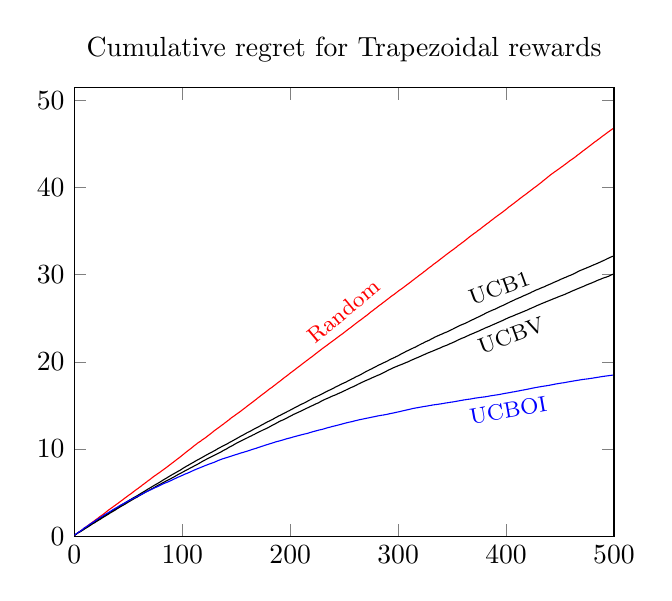
\begin{tikzpicture}
	\begin{axis}[
		title={Cumulative regret for Trapezoidal rewards},
		%xlabel={Total number of pulls},
		xmin=0, xmax=500,
		ymin=0, %ymax=20,
	%	ymajorgrids=true,
		grid style=dashed
	]
	\addplot[red] coordinates {
(0,0.0831643558341)(1,0.174778668555)(2,0.262987471382)(3,0.347403668354)(4,0.435739445949)(5,0.526613713815)(6,0.627085757389)(7,0.714170815242)(8,0.801690884253)(9,0.891041511397)(10,0.993009667105)(11,1.0876633326)(12,1.17925264791)(13,1.26426598616)(14,1.34567914119)(15,1.4424813437)(16,1.52753171554)(17,1.62492664215)(18,1.71353293274)(19,1.81487171283)(20,1.91112437567)(21,1.98968963091)(22,2.0792450054)(23,2.18860118891)(24,2.27448031398)(25,2.35511692067)(26,2.44819509778)(27,2.53434167376)(28,2.63043568379)(29,2.73250917227)(30,2.83072388466)(31,2.93498901581)(32,3.02495130438)(33,3.1118983472)(34,3.20206028695)(35,3.28266580233)(36,3.3842286517)(37,3.46812930103)(38,3.55705154425)(39,3.64895756805)(40,3.73738719714)(41,3.83076850375)(42,3.92655020803)(43,4.01049658936)(44,4.10495508583)(45,4.19198923137)(46,4.29074282952)(47,4.3889574531)(48,4.47782714042)(49,4.57060703825)(50,4.66698566189)(51,4.74930795927)(52,4.83213368378)(53,4.92057432377)(54,5.02591749752)(55,5.11637689919)(56,5.21494272502)(57,5.30499609628)(58,5.3954529373)(59,5.47406651218)(60,5.57920940239)(61,5.66670096414)(62,5.75886815825)(63,5.86251436089)(64,5.94684723955)(65,6.0408430593)(66,6.13944341589)(67,6.22930900724)(68,6.33032090657)(69,6.41450708556)(70,6.50512887001)(71,6.60267055781)(72,6.69770790963)(73,6.79683698407)(74,6.88792210277)(75,6.97575086455)(76,7.05618754763)(77,7.1448489476)(78,7.22855062154)(79,7.31434017051)(80,7.40387981229)(81,7.4978301604)(82,7.58632660523)(83,7.68013292313)(84,7.76646638723)(85,7.85203903689)(86,7.94708814601)(87,8.0480880294)(88,8.140722584)(89,8.23549134511)(90,8.32878099905)(91,8.42639064347)(92,8.51262685335)(93,8.61512652852)(94,8.7083789206)(95,8.80632393188)(96,8.89507183444)(97,8.98795571028)(98,9.0819858689)(99,9.18549459156)(100,9.28579966536)(101,9.38334633557)(102,9.49202757396)(103,9.5891893613)(104,9.6810063436)(105,9.78491630619)(106,9.87565203847)(107,9.96946794055)(108,10.0615675731)(109,10.1618325245)(110,10.2635465591)(111,10.3683215962)(112,10.4608630808)(113,10.556154047)(114,10.6529828311)(115,10.7472435353)(116,10.820437338)(117,10.8999913928)(118,11.0035545435)(119,11.0877365301)(120,11.1771979611)(121,11.252697289)(122,11.3444860187)(123,11.4447625635)(124,11.5441760971)(125,11.6373487435)(126,11.7308499576)(127,11.829951029)(128,11.925110649)(129,12.0335513018)(130,12.129620654)(131,12.2147667125)(132,12.3063175435)(133,12.3946753855)(134,12.4861006921)(135,12.5758747596)(136,12.6719900748)(137,12.7630683991)(138,12.8495373697)(139,12.9497902235)(140,13.0424639943)(141,13.1350236049)(142,13.2340067717)(143,13.3200468536)(144,13.4216461128)(145,13.5314619937)(146,13.6252358603)(147,13.7075792606)(148,13.7926942728)(149,13.8862128709)(150,13.9697424496)(151,14.0618888209)(152,14.1448389281)(153,14.2383637096)(154,14.3241256347)(155,14.4230509603)(156,14.5201287998)(157,14.6149678237)(158,14.704799269)(159,14.8029287685)(160,14.9067972708)(161,14.9960027159)(162,15.0866584808)(163,15.186932993)(164,15.2776744632)(165,15.3635060403)(166,15.4648555064)(167,15.5612851598)(168,15.6553636467)(169,15.7529840017)(170,15.8572478873)(171,15.9485879354)(172,16.0461323636)(173,16.1482655496)(174,16.2363690765)(175,16.3312452398)(176,16.420376984)(177,16.5117388978)(178,16.6109229084)(179,16.7062403603)(180,16.810140086)(181,16.9040158496)(182,16.9832056777)(183,17.0684593403)(184,17.1696309535)(185,17.2641017112)(186,17.3551382769)(187,17.4528118734)(188,17.5585366774)(189,17.6510744701)(190,17.7297535963)(191,17.8365925858)(192,17.9316137949)(193,18.0291328101)(194,18.1312112753)(195,18.2307788174)(196,18.3109893732)(197,18.4081749657)(198,18.4974970802)(199,18.6117217511)(200,18.7035828464)(201,18.7946925152)(202,18.8845386962)(203,18.9842463397)(204,19.0669316863)(205,19.1697810456)(206,19.2685535685)(207,19.3632306707)(208,19.4555539347)(209,19.5410234962)(210,19.6408376549)(211,19.7384671772)(212,19.8359170518)(213,19.9292869575)(214,20.0202485001)(215,20.118541083)(216,20.2084840909)(217,20.2990454657)(218,20.398255278)(219,20.4917510041)(220,20.5672677731)(221,20.6695931831)(222,20.7710466305)(223,20.8668734051)(224,20.9698968483)(225,21.0582430991)(226,21.1564818134)(227,21.25206598)(228,21.3436417619)(229,21.4383381134)(230,21.5408429539)(231,21.6260974517)(232,21.715803579)(233,21.8063137932)(234,21.8952001441)(235,21.9926281036)(236,22.0815609888)(237,22.1750931775)(238,22.2666436724)(239,22.3521709909)(240,22.4492497538)(241,22.5352373846)(242,22.6332873819)(243,22.7221228407)(244,22.8252121019)(245,22.9098558589)(246,23.003759189)(247,23.0914110733)(248,23.1792223956)(249,23.2717904727)(250,23.370467345)(251,23.4646861836)(252,23.5634343172)(253,23.6610239434)(254,23.755730284)(255,23.8465171182)(256,23.9340359187)(257,24.0322520475)(258,24.1236402547)(259,24.2291915653)(260,24.3232537665)(261,24.4183550479)(262,24.514845045)(263,24.6057652768)(264,24.7045422101)(265,24.7815753069)(266,24.8725513937)(267,24.9736386275)(268,25.0653285457)(269,25.1605297039)(270,25.2518895805)(271,25.342413583)(272,25.4383753878)(273,25.5450633892)(274,25.6506261315)(275,25.7479949624)(276,25.8350998428)(277,25.9272710376)(278,26.0315831711)(279,26.121587967)(280,26.2152206106)(281,26.317891209)(282,26.4104039408)(283,26.5076828302)(284,26.5926525455)(285,26.6863977378)(286,26.7880779025)(287,26.8781653123)(288,26.9717057486)(289,27.0715767143)(290,27.1659871531)(291,27.2579850173)(292,27.3537482113)(293,27.4545834386)(294,27.5448570147)(295,27.6378403109)(296,27.7125284479)(297,27.8096613487)(298,27.9019649147)(299,28.0067480197)(300,28.1021981774)(301,28.1959684201)(302,28.2833738454)(303,28.3557270865)(304,28.4485205946)(305,28.5388729361)(306,28.6411296352)(307,28.7260285921)(308,28.8243830394)(309,28.915760092)(310,29.0090490005)(311,29.1107668116)(312,29.1919928333)(313,29.2958013393)(314,29.3883417092)(315,29.4815219567)(316,29.5836998477)(317,29.6723597611)(318,29.7675266618)(319,29.8669629709)(320,29.9595262369)(321,30.0476234493)(322,30.1437298126)(323,30.2337371614)(324,30.3386840913)(325,30.4275298796)(326,30.5267010329)(327,30.6305780203)(328,30.7240935835)(329,30.8195646564)(330,30.9160424332)(331,30.9999831298)(332,31.1067229666)(333,31.2040762345)(334,31.2947120637)(335,31.380092289)(336,31.4717861885)(337,31.5677235821)(338,31.6676638154)(339,31.7639347662)(340,31.8600874174)(341,31.9481227013)(342,32.0472956189)(343,32.1422774398)(344,32.2409642767)(345,32.3303751556)(346,32.4299963448)(347,32.5160960125)(348,32.6093460934)(349,32.7082388884)(350,32.7923875006)(351,32.87410433)(352,32.9672453372)(353,33.0707549418)(354,33.1583283931)(355,33.2675304539)(356,33.3603649823)(357,33.4522353549)(358,33.537680145)(359,33.6378284286)(360,33.729817392)(361,33.8214116588)(362,33.9180816082)(363,34.0159611085)(364,34.1168972504)(365,34.2189689583)(366,34.321420588)(367,34.4111534882)(368,34.5025292942)(369,34.5998588808)(370,34.694532392)(371,34.7729105539)(372,34.8607494049)(373,34.9605026923)(374,35.059831062)(375,35.1392579478)(376,35.2284835343)(377,35.3326999357)(378,35.4330715686)(379,35.5269883188)(380,35.617175551)(381,35.7224727897)(382,35.8116846346)(383,35.902164644)(384,35.9898259691)(385,36.0950330465)(386,36.197046333)(387,36.2829986721)(388,36.3780554793)(389,36.4746990743)(390,36.5675323882)(391,36.6566483667)(392,36.7548831398)(393,36.8424697928)(394,36.9288426353)(395,37.0220127088)(396,37.1102892856)(397,37.1954407929)(398,37.2960865292)(399,37.3898863228)(400,37.4900698631)(401,37.5915726033)(402,37.6939380642)(403,37.7971289205)(404,37.8824149401)(405,37.9756994869)(406,38.0743923321)(407,38.1607454377)(408,38.2562097571)(409,38.3573198838)(410,38.4477983731)(411,38.5453986326)(412,38.647411916)(413,38.7460199886)(414,38.8333233179)(415,38.9281065538)(416,39.0299592981)(417,39.1066985307)(418,39.197394875)(419,39.2896598712)(420,39.3963252952)(421,39.4845666725)(422,39.5738080774)(423,39.6750773049)(424,39.7637579493)(425,39.8608548174)(426,39.9611532291)(427,40.0484219827)(428,40.1316626265)(429,40.231091676)(430,40.3300181562)(431,40.428882598)(432,40.5195532977)(433,40.6169549996)(434,40.7283679688)(435,40.8279713058)(436,40.9255366196)(437,41.0204625561)(438,41.12208915)(439,41.2261134279)(440,41.3260236381)(441,41.4289895516)(442,41.5225519275)(443,41.6094449528)(444,41.6997901838)(445,41.7894541188)(446,41.8721164619)(447,41.9610244972)(448,42.0456773277)(449,42.1335639847)(450,42.2298466547)(451,42.3223936585)(452,42.4016253918)(453,42.4911067834)(454,42.5908246629)(455,42.6778301216)(456,42.7636511941)(457,42.8674417399)(458,42.9646017421)(459,43.0588925286)(460,43.146382379)(461,43.2305439176)(462,43.3132360653)(463,43.3966709028)(464,43.4894841886)(465,43.5833759391)(466,43.6960250054)(467,43.7785814454)(468,43.8745439423)(469,43.9704047111)(470,44.0617368564)(471,44.1694147014)(472,44.2565349162)(473,44.3505159198)(474,44.447197388)(475,44.5308456513)(476,44.6344047101)(477,44.7307296451)(478,44.8209427997)(479,44.9149425737)(480,45.0117158808)(481,45.1115041223)(482,45.206508497)(483,45.29079553)(484,45.3771609594)(485,45.4748164882)(486,45.5622965794)(487,45.6549265749)(488,45.7555795121)(489,45.85005994)(490,45.9447407156)(491,46.0270133907)(492,46.1215696981)(493,46.2142197811)(494,46.3090020423)(495,46.3963860409)(496,46.4822650497)(497,46.5728835693)(498,46.6665923469)(499,46.7505210823)
		}node[pos=0.52](endofplotsquare){} ;
		\node [red,above,rotate=40] at (endofplotsquare) {\footnotesize Random};
	\addplot[black] coordinates {
(0,0.0890003360078)(1,0.175641731596)(2,0.26818273857)(3,0.359782498838)(4,0.443315391255)(5,0.502744182118)(6,0.579736571491)(7,0.657741402146)(8,0.760577691071)(9,0.86913655711)(10,0.937541882727)(11,0.992124448184)(12,1.06246930522)(13,1.14509901248)(14,1.23604249166)(15,1.32282929187)(16,1.4047816666)(17,1.484640138)(18,1.55787330301)(19,1.64259966004)(20,1.73126046333)(21,1.80715225)(22,1.88952671872)(23,1.97196763677)(24,2.04373771455)(25,2.1224781698)(26,2.20389790211)(27,2.28749029103)(28,2.36824935756)(29,2.44231007083)(30,2.51666949322)(31,2.59450225559)(32,2.67676384504)(33,2.74559277481)(34,2.82225126837)(35,2.89760218879)(36,2.98101506766)(37,3.06253145684)(38,3.13755266223)(39,3.21947326014)(40,3.29624202098)(41,3.37024602259)(42,3.44808033926)(43,3.52646949124)(44,3.60230179814)(45,3.67649150188)(46,3.74425776633)(47,3.81284554328)(48,3.88805680775)(49,3.97417196204)(50,4.05471657677)(51,4.13457978126)(52,4.19872647363)(53,4.27263802805)(54,4.35234724357)(55,4.43300937533)(56,4.49125767727)(57,4.5616042812)(58,4.62909742546)(59,4.7044852544)(60,4.78215769194)(61,4.86149069536)(62,4.9384573916)(63,5.01361785273)(64,5.08124771895)(65,5.14992000845)(66,5.23199884515)(67,5.30922698928)(68,5.38760799709)(69,5.45991700854)(70,5.53471005217)(71,5.60679126526)(72,5.67689551805)(73,5.75839961115)(74,5.83325646445)(75,5.903247323)(76,5.97576028999)(77,6.04118146656)(78,6.10758878098)(79,6.1857719109)(80,6.26222291711)(81,6.34109993056)(82,6.42523996688)(83,6.49134033129)(84,6.57358354653)(85,6.63931586819)(86,6.71475041115)(87,6.79137614968)(88,6.8679364899)(89,6.94379176032)(90,7.01277181099)(91,7.08826560542)(92,7.14878157186)(93,7.22055125213)(94,7.29143605768)(95,7.36437498421)(96,7.44346165193)(97,7.50555882528)(98,7.56998620018)(99,7.64539939302)(100,7.7309002754)(101,7.81435324407)(102,7.88406769473)(103,7.96476180281)(104,8.03850476055)(105,8.09969308025)(106,8.16930866886)(107,8.24524980372)(108,8.31361991858)(109,8.38328143633)(110,8.45128418482)(111,8.52895933299)(112,8.60218636491)(113,8.67094757032)(114,8.73802980339)(115,8.80782222758)(116,8.87036568573)(117,8.9410450186)(118,9.00725725869)(119,9.07643627938)(120,9.14834738109)(121,9.22351946185)(122,9.28915146941)(123,9.35740858297)(124,9.42500955578)(125,9.48902726176)(126,9.55312451219)(127,9.61432061515)(128,9.68517517583)(129,9.75395990782)(130,9.81454703152)(131,9.88755083251)(132,9.96316637261)(133,10.0445016017)(134,10.1107330659)(135,10.1749413622)(136,10.2403354683)(137,10.3033845548)(138,10.3734623987)(139,10.4351106412)(140,10.4919585387)(141,10.5552472402)(142,10.6217279109)(143,10.6992032379)(144,10.7695781426)(145,10.8357796739)(146,10.9004687817)(147,10.9669972474)(148,11.039152063)(149,11.1114490214)(150,11.171951978)(151,11.2484193547)(152,11.3144650029)(153,11.3880470523)(154,11.4596950274)(155,11.5265825825)(156,11.5884132569)(157,11.6537634456)(158,11.7239082036)(159,11.7945080606)(160,11.8687054771)(161,11.9299776129)(162,11.9868985511)(163,12.0486039945)(164,12.1122833085)(165,12.1885361605)(166,12.2523984187)(167,12.3200196694)(168,12.3829708533)(169,12.4451224506)(170,12.510083621)(171,12.5742449203)(172,12.6420893433)(173,12.7154083634)(174,12.7914950776)(175,12.8458869544)(176,12.9149554752)(177,12.9889202605)(178,13.0483478597)(179,13.1198546247)(180,13.1767621634)(181,13.2342911406)(182,13.3020128037)(183,13.3619404808)(184,13.4212685411)(185,13.4903216614)(186,13.5695020657)(187,13.6368719082)(188,13.7008138651)(189,13.7694819827)(190,13.8258698318)(191,13.8854160634)(192,13.9540707759)(193,14.0246483983)(194,14.0784427126)(195,14.1453780823)(196,14.2079106448)(197,14.2728213447)(198,14.3371567776)(199,14.3958304737)(200,14.4594274441)(201,14.5269147469)(202,14.5916739621)(203,14.6580365378)(204,14.7240949363)(205,14.7872124993)(206,14.8494763952)(207,14.9145264643)(208,14.9852080389)(209,15.0498658193)(210,15.1163393303)(211,15.1724795106)(212,15.2233621558)(213,15.2778505326)(214,15.3422628857)(215,15.4056246204)(216,15.4800302528)(217,15.5525862658)(218,15.6166339297)(219,15.6774331416)(220,15.7513940839)(221,15.8235466873)(222,15.8801530834)(223,15.9392047846)(224,15.9933441271)(225,16.0492725664)(226,16.1123595889)(227,16.1687982666)(228,16.2283346606)(229,16.2931189278)(230,16.3482384577)(231,16.4190145885)(232,16.4895671253)(233,16.5500616391)(234,16.6178048508)(235,16.6755339231)(236,16.7349174034)(237,16.7883881215)(238,16.847032419)(239,16.9135476201)(240,16.9767102126)(241,17.0350740461)(242,17.1174237166)(243,17.1682652702)(244,17.2284246492)(245,17.2817106374)(246,17.3569077258)(247,17.4196340986)(248,17.4812345446)(249,17.5328300337)(250,17.5918683587)(251,17.6426585129)(252,17.7002788605)(253,17.772055112)(254,17.8364870768)(255,17.899381352)(256,17.9646281078)(257,18.0326267322)(258,18.0854507934)(259,18.1512350877)(260,18.2195843588)(261,18.2925905293)(262,18.3459066716)(263,18.3942533495)(264,18.4619639111)(265,18.5178209824)(266,18.5856511897)(267,18.6564925837)(268,18.7266445329)(269,18.7984302804)(270,18.8666072914)(271,18.9303615143)(272,18.9876100456)(273,19.049514958)(274,19.1236424937)(275,19.1706897296)(276,19.2270086798)(277,19.3076259448)(278,19.3699226175)(279,19.4321092683)(280,19.4920437396)(281,19.5670618032)(282,19.6327302586)(283,19.6802767474)(284,19.7352186653)(285,19.7997813429)(286,19.859895524)(287,19.9198166635)(288,19.9680768842)(289,20.0281372581)(290,20.085734181)(291,20.1617623722)(292,20.2288448545)(293,20.2887127737)(294,20.3526436737)(295,20.3990986048)(296,20.4619290064)(297,20.5189415098)(298,20.5899836683)(299,20.6442545928)(300,20.7046248201)(301,20.771623054)(302,20.8428336657)(303,20.9135637825)(304,20.9784845581)(305,21.0324107837)(306,21.0999440158)(307,21.1756603804)(308,21.2321799927)(309,21.2905246917)(310,21.3520345285)(311,21.4099754353)(312,21.470446273)(313,21.5250854522)(314,21.5880179241)(315,21.6375351262)(316,21.6926195913)(317,21.7615966833)(318,21.8295901227)(319,21.8978595679)(320,21.9589330222)(321,22.0212958737)(322,22.0871500533)(323,22.1426967207)(324,22.2083327058)(325,22.2724420786)(326,22.3337916581)(327,22.3835576534)(328,22.4393124874)(329,22.4946525874)(330,22.5661975802)(331,22.6334998803)(332,22.6931324132)(333,22.7616631251)(334,22.8299050067)(335,22.8871523449)(336,22.9380102712)(337,23.0003173274)(338,23.0501342635)(339,23.1101848941)(340,23.1603133576)(341,23.2109709224)(342,23.2737867069)(343,23.3239113653)(344,23.3744266403)(345,23.4211879748)(346,23.4734956382)(347,23.5431073525)(348,23.6010246457)(349,23.6582829431)(350,23.7161123202)(351,23.7780435344)(352,23.8411838266)(353,23.9032260079)(354,23.9666846594)(355,24.0346361485)(356,24.0952954702)(357,24.1593611396)(358,24.2131306319)(359,24.2614136393)(360,24.3092163776)(361,24.3595221103)(362,24.4071183019)(363,24.465820705)(364,24.5269991826)(365,24.5867080581)(366,24.6507870229)(367,24.7171042614)(368,24.7768519207)(369,24.835976113)(370,24.8864088671)(371,24.949716768)(372,25.0124722765)(373,25.0754242022)(374,25.1274630893)(375,25.1855888847)(376,25.2417784201)(377,25.3075216315)(378,25.3697310635)(379,25.423768961)(380,25.5018923984)(381,25.5723746792)(382,25.6300018822)(383,25.6872239522)(384,25.7413208249)(385,25.7969501838)(386,25.8577137727)(387,25.9100874827)(388,25.9605128432)(389,26.0038844025)(390,26.0554774085)(391,26.1132434224)(392,26.1805187667)(393,26.2432350853)(394,26.2978339023)(395,26.3595327625)(396,26.4155190814)(397,26.462368223)(398,26.5250845183)(399,26.5870989005)(400,26.6451718232)(401,26.7023238937)(402,26.7635744653)(403,26.8242429943)(404,26.889149195)(405,26.9411601209)(406,27.0027400815)(407,27.0569540703)(408,27.1193297516)(409,27.1825445844)(410,27.2269390051)(411,27.282580258)(412,27.3408337096)(413,27.3822817021)(414,27.4364063687)(415,27.5020364459)(416,27.5615407099)(417,27.6176162653)(418,27.6643705074)(419,27.7207303636)(420,27.7759474528)(421,27.8347487522)(422,27.8853585051)(423,27.9462715663)(424,28.0128961889)(425,28.0681505762)(426,28.1277904935)(427,28.1884562443)(428,28.2437898553)(429,28.2911609144)(430,28.3380241068)(431,28.3948831926)(432,28.4513206515)(433,28.5003127595)(434,28.5471246165)(435,28.5895326167)(436,28.6500362364)(437,28.7162293301)(438,28.7663346141)(439,28.8190121437)(440,28.8790592019)(441,28.9226908771)(442,28.9775607586)(443,29.0420747826)(444,29.0990112677)(445,29.1487617358)(446,29.2027668238)(447,29.2563110791)(448,29.3042036355)(449,29.3661302197)(450,29.4196672502)(451,29.4825008541)(452,29.538027454)(453,29.5865296167)(454,29.6402229876)(455,29.6832694555)(456,29.7343255651)(457,29.7980484178)(458,29.8498497999)(459,29.898428014)(460,29.9468555464)(461,29.9992776489)(462,30.0533421578)(463,30.1216034549)(464,30.1792909211)(465,30.2430978271)(466,30.3104997215)(467,30.378636298)(468,30.4363733618)(469,30.4878933285)(470,30.5405151493)(471,30.5936970205)(472,30.6458681101)(473,30.6888434282)(474,30.7381803658)(475,30.7967646159)(476,30.8436600514)(477,30.8936871662)(478,30.9475518494)(479,31.0048096574)(480,31.0588689638)(481,31.1165027042)(482,31.1628863636)(483,31.2129964053)(484,31.2648113294)(485,31.3220594652)(486,31.3761447359)(487,31.4304941415)(488,31.4838818143)(489,31.5480846016)(490,31.5999437397)(491,31.6561681668)(492,31.7174862926)(493,31.7781870393)(494,31.8442310839)(495,31.8988914535)(496,31.9548073011)(497,32.0132993022)(498,32.069496733)(499,32.1204586135)
		}node[pos=0.8](endofplotsquare){} ;
		\node [black,above,rotate=20] at (endofplotsquare) {\footnotesize UCB1};
	\addplot[black] coordinates {
(0,0.0762420395718)(1,0.176847885478)(2,0.268798855409)(3,0.356061997509)(4,0.438549453175)(5,0.484771872509)(6,0.561935285108)(7,0.633954494979)(8,0.709303763784)(9,0.79164295235)(10,0.872019222374)(11,0.947716701673)(12,1.01996034238)(13,1.09826236453)(14,1.17889837772)(15,1.25714945884)(16,1.34811047777)(17,1.42801315581)(18,1.49818270815)(19,1.55830106796)(20,1.64705601513)(21,1.72381150589)(22,1.79778217061)(23,1.86994216858)(24,1.93382971852)(25,2.02273609075)(26,2.11185169818)(27,2.186065159)(28,2.25541190061)(29,2.33075628462)(30,2.41292223197)(31,2.48249523473)(32,2.56598087999)(33,2.65001571146)(34,2.7177340266)(35,2.79543539399)(36,2.86835255955)(37,2.93636870287)(38,3.00912819369)(39,3.09926762147)(40,3.17040716922)(41,3.24607957848)(42,3.32234181263)(43,3.39882711613)(44,3.47290758284)(45,3.53275621867)(46,3.60702522473)(47,3.67911253785)(48,3.75624898038)(49,3.82856660433)(50,3.91217933772)(51,3.98487614598)(52,4.0538990177)(53,4.12823830708)(54,4.203587354)(55,4.27330689908)(56,4.34994786566)(57,4.41066673539)(58,4.47622293599)(59,4.54544980473)(60,4.63033961605)(61,4.69771088512)(62,4.77159681596)(63,4.83319961819)(64,4.91810068495)(65,4.98622155092)(66,5.05302344906)(67,5.11406635074)(68,5.18598175476)(69,5.23617848074)(70,5.31318036704)(71,5.38685724107)(72,5.45014526274)(73,5.51988613809)(74,5.58325321839)(75,5.65931531662)(76,5.73369185309)(77,5.80563975074)(78,5.86021917682)(79,5.93003828961)(80,5.99011308767)(81,6.0697657753)(82,6.12692180452)(83,6.19327992042)(84,6.25996964221)(85,6.33181698027)(86,6.39533204183)(87,6.45706386193)(88,6.51677099755)(89,6.58200944288)(90,6.64370372041)(91,6.71302243867)(92,6.77928279241)(93,6.84242234112)(94,6.92311235351)(95,6.99426780917)(96,7.06607546016)(97,7.12583798567)(98,7.19291408208)(99,7.25783414774)(100,7.32091336125)(101,7.39423372517)(102,7.45735065514)(103,7.5353114069)(104,7.59534928588)(105,7.65691072969)(106,7.72146116356)(107,7.79132604254)(108,7.85422328091)(109,7.91380026701)(110,7.98077350014)(111,8.04852180933)(112,8.11253599644)(113,8.17692702605)(114,8.24488843819)(115,8.31025056071)(116,8.38774791317)(117,8.45569833055)(118,8.53257178637)(119,8.60311224159)(120,8.67459603434)(121,8.73673485175)(122,8.79890424773)(123,8.8693910659)(124,8.93539038314)(125,8.99559022645)(126,9.05289532774)(127,9.11909379322)(128,9.17896981575)(129,9.24123721868)(130,9.30127050649)(131,9.36033794766)(132,9.42664139087)(133,9.49170226202)(134,9.55051191437)(135,9.61162858218)(136,9.67779200431)(137,9.75409498554)(138,9.82166707055)(139,9.88653667749)(140,9.95533534491)(141,10.0158138874)(142,10.0873056187)(143,10.1716412217)(144,10.2420249345)(145,10.3031064824)(146,10.3648090504)(147,10.4308863841)(148,10.5127557972)(149,10.582586933)(150,10.6484163836)(151,10.712204741)(152,10.7821966067)(153,10.8432297601)(154,10.9086184797)(155,10.9620450027)(156,11.0288297573)(157,11.0853565537)(158,11.1476266251)(159,11.2159447744)(160,11.2659283341)(161,11.3291404388)(162,11.3949943154)(163,11.4559987857)(164,11.5049161435)(165,11.5770994568)(166,11.638367983)(167,11.6939176189)(168,11.7700431109)(169,11.8335880794)(170,11.8961710353)(171,11.9600396809)(172,12.0174555654)(173,12.0708903604)(174,12.1336044321)(175,12.1942654131)(176,12.2457237337)(177,12.3023032)(178,12.3644160865)(179,12.4206554918)(180,12.4870719018)(181,12.5540070093)(182,12.6237227147)(183,12.6934084928)(184,12.7540520147)(185,12.8149248643)(186,12.8818328203)(187,12.9531509034)(188,13.0237080331)(189,13.0909292362)(190,13.1559936406)(191,13.2180651845)(192,13.2728533021)(193,13.3199721294)(194,13.3780223817)(195,13.4387526796)(196,13.5016781883)(197,13.5692397226)(198,13.6322723131)(199,13.7048646724)(200,13.7629561174)(201,13.8284047233)(202,13.8916525426)(203,13.96496316)(204,14.0174767486)(205,14.0705607582)(206,14.1325858365)(207,14.1786164224)(208,14.2403772608)(209,14.297506303)(210,14.3603607674)(211,14.4179534596)(212,14.4793438929)(213,14.5369980783)(214,14.5940869199)(215,14.6619862182)(216,14.7177184009)(217,14.7694371773)(218,14.8334350322)(219,14.8991299305)(220,14.9516590054)(221,15.0102968232)(222,15.0721079125)(223,15.1325755439)(224,15.1911234637)(225,15.2399164866)(226,15.2837015793)(227,15.3574611597)(228,15.4307607154)(229,15.5053818783)(230,15.5668556759)(231,15.6290946315)(232,15.682018878)(233,15.7412031636)(234,15.7891883909)(235,15.8421185078)(236,15.8962517901)(237,15.9558721362)(238,16.0183601027)(239,16.0663877855)(240,16.1191529265)(241,16.1595114584)(242,16.2126109504)(243,16.2723534515)(244,16.3374898751)(245,16.3820365515)(246,16.4356876885)(247,16.492142947)(248,16.5485313186)(249,16.608390263)(250,16.6694454069)(251,16.7242322261)(252,16.7897177039)(253,16.8483770178)(254,16.9096742792)(255,16.9737477542)(256,17.0275478417)(257,17.0799916541)(258,17.1286953982)(259,17.1886201158)(260,17.2492319219)(261,17.3071727294)(262,17.3776116552)(263,17.4412577169)(264,17.5013441064)(265,17.5586979578)(266,17.6143281484)(267,17.6785054724)(268,17.7301457381)(269,17.7921339155)(270,17.8466575942)(271,17.9003630238)(272,17.9527257655)(273,18.0049987684)(274,18.0543159027)(275,18.1227329597)(276,18.176089883)(277,18.2302339217)(278,18.2812971305)(279,18.3331525881)(280,18.3923180536)(281,18.4521258599)(282,18.4898632878)(283,18.5464364328)(284,18.6060824984)(285,18.6665035048)(286,18.7321451252)(287,18.7944679431)(288,18.8492589915)(289,18.920457536)(290,18.9853441061)(291,19.0515467532)(292,19.1134235111)(293,19.1637836396)(294,19.2255685787)(295,19.2888809051)(296,19.3403534263)(297,19.392041576)(298,19.445355089)(299,19.4923530073)(300,19.5527129023)(301,19.6007265227)(302,19.6478544152)(303,19.6915344069)(304,19.744284733)(305,19.7917006097)(306,19.8457026598)(307,19.9025396976)(308,19.9500358993)(309,19.994702573)(310,20.0556843757)(311,20.1116542533)(312,20.1751013023)(313,20.2313738722)(314,20.2826447361)(315,20.3398262505)(316,20.3851412959)(317,20.441300229)(318,20.4924084487)(319,20.5441094773)(320,20.597437552)(321,20.6569797588)(322,20.7163174567)(323,20.7682724802)(324,20.8236884301)(325,20.8735908111)(326,20.9361067294)(327,20.9896181683)(328,21.0393363768)(329,21.091240541)(330,21.1402518263)(331,21.1875155456)(332,21.2331368881)(333,21.2886177232)(334,21.3461730206)(335,21.3938506161)(336,21.4481548572)(337,21.4993495451)(338,21.545749554)(339,21.5944718841)(340,21.6519005044)(341,21.7148658077)(342,21.7673339872)(343,21.816848334)(344,21.859020059)(345,21.9046367374)(346,21.956221718)(347,22.0130320032)(348,22.0749887074)(349,22.124390266)(350,22.1754130463)(351,22.2326531473)(352,22.2868659046)(353,22.3453474575)(354,22.4078654477)(355,22.4769868873)(356,22.5338156024)(357,22.5891349319)(358,22.6422795277)(359,22.6993852755)(360,22.7462592631)(361,22.7873456191)(362,22.8441301961)(363,22.9072765457)(364,22.9659899985)(365,23.0165093799)(366,23.0789387598)(367,23.1402004104)(368,23.1873245605)(369,23.2376833981)(370,23.2839760869)(371,23.3461815129)(372,23.390444642)(373,23.4464057687)(374,23.4976664461)(375,23.5549217928)(376,23.6129418611)(377,23.669204073)(378,23.7292661267)(379,23.7761636475)(380,23.8393802106)(381,23.8990851325)(382,23.9476670511)(383,23.9998346949)(384,24.0382961594)(385,24.0941891659)(386,24.1540635988)(387,24.212623628)(388,24.2681558323)(389,24.3207401243)(390,24.3721140563)(391,24.4219337361)(392,24.482727684)(393,24.5346034479)(394,24.5875962334)(395,24.6433069589)(396,24.699459829)(397,24.7523785102)(398,24.8217668579)(399,24.8791927756)(400,24.9385095318)(401,24.9909922623)(402,25.0475651498)(403,25.1046957185)(404,25.1544836187)(405,25.198699118)(406,25.2437302307)(407,25.2942506043)(408,25.3492320817)(409,25.4093685774)(410,25.4616614094)(411,25.5034605586)(412,25.5559455755)(413,25.6029671431)(414,25.6504204157)(415,25.7064947355)(416,25.7573007149)(417,25.8105392502)(418,25.8643322772)(419,25.9085221029)(420,25.9630819739)(421,26.027714861)(422,26.0849185847)(423,26.1354545526)(424,26.191925324)(425,26.2425670782)(426,26.2980712771)(427,26.3556259904)(428,26.4149673735)(429,26.4703876513)(430,26.5181603531)(431,26.5725075867)(432,26.6278117864)(433,26.6831402971)(434,26.7275528912)(435,26.7786759129)(436,26.8275838293)(437,26.8837442975)(438,26.9365370777)(439,26.9808014467)(440,27.0301621469)(441,27.0860476587)(442,27.1283111528)(443,27.1863632123)(444,27.2375405309)(445,27.2846346847)(446,27.3292407251)(447,27.3782945155)(448,27.4354737557)(449,27.481634255)(450,27.5320420638)(451,27.5799037242)(452,27.6205420347)(453,27.6692546552)(454,27.7165090518)(455,27.7723914035)(456,27.8346970475)(457,27.8889083295)(458,27.9342273733)(459,27.990928854)(460,28.0448901446)(461,28.1087015253)(462,28.1610227326)(463,28.2119173292)(464,28.2606944486)(465,28.3211464637)(466,28.3689563229)(467,28.4144146435)(468,28.4693204218)(469,28.5235005042)(470,28.5732530428)(471,28.6192925493)(472,28.6721144882)(473,28.7277375661)(474,28.787897476)(475,28.842103927)(476,28.89002421)(477,28.9436081307)(478,28.9824010867)(479,29.0342706736)(480,29.0882649421)(481,29.1418977005)(482,29.1876666877)(483,29.2450258604)(484,29.3046014079)(485,29.3594842572)(486,29.4069815561)(487,29.4491245555)(488,29.5030786163)(489,29.5581846445)(490,29.6049138532)(491,29.6500414667)(492,29.6874956966)(493,29.7286059731)(494,29.7715789844)(495,29.8204960598)(496,29.8747091354)(497,29.9415967124)(498,29.9976850542)(499,30.0510595846)
		}node[pos=0.8](endofplotsquare){} ;
		\node [black,below,rotate=20] at (endofplotsquare) {\footnotesize UCBV};
	\addplot[blue] coordinates {
(0,0.103088510766)(1,0.197405899114)(2,0.287623793052)(3,0.371432739706)(4,0.471831075885)(5,0.536619393096)(6,0.615321929798)(7,0.71016093862)(8,0.813608794324)(9,0.94136746047)(10,0.994976038228)(11,1.06794130333)(12,1.15795599707)(13,1.24153325579)(14,1.34010732246)(15,1.43074702333)(16,1.49864139477)(17,1.57583327114)(18,1.65260377923)(19,1.74169475922)(20,1.82380725874)(21,1.9088601089)(22,1.9903589263)(23,2.07032107323)(24,2.14979423099)(25,2.21898779748)(26,2.29657578528)(27,2.37649311967)(28,2.45049581845)(29,2.53117208022)(30,2.60816620167)(31,2.67864605674)(32,2.7455698587)(33,2.82040122242)(34,2.90124475631)(35,2.97598197279)(36,3.06080374738)(37,3.12966490817)(38,3.20815031857)(39,3.27161237637)(40,3.34306718793)(41,3.41908967623)(42,3.50120729929)(43,3.56719754146)(44,3.63889245906)(45,3.70195603751)(46,3.77214615138)(47,3.84450474151)(48,3.90442174776)(49,3.96906941024)(50,4.03474159438)(51,4.10584100394)(52,4.17438214558)(53,4.23701007932)(54,4.30117555942)(55,4.35660838705)(56,4.41274804225)(57,4.4750196352)(58,4.53407436822)(59,4.59544220795)(60,4.65694577932)(61,4.71701916845)(62,4.78409517487)(63,4.84009436584)(64,4.91027970625)(65,4.97357667109)(66,5.05366513573)(67,5.11116947001)(68,5.16324689673)(69,5.22328964516)(70,5.28028224901)(71,5.33903717276)(72,5.39968637092)(73,5.45957239684)(74,5.51386299377)(75,5.57757708083)(76,5.63229745259)(77,5.68058848057)(78,5.74166239834)(79,5.8025597468)(80,5.85869776375)(81,5.92118015311)(82,5.98321339981)(83,6.04160029778)(84,6.09455562279)(85,6.14305314925)(86,6.19600406095)(87,6.23887546422)(88,6.30010354236)(89,6.35478737361)(90,6.4051672931)(91,6.46568603742)(92,6.53995271559)(93,6.58906374176)(94,6.6436700518)(95,6.70089279985)(96,6.76215968026)(97,6.81997573867)(98,6.86609367938)(99,6.92371333303)(100,6.97782794847)(101,7.03625435524)(102,7.09531762955)(103,7.14558718591)(104,7.18639517388)(105,7.23992743385)(106,7.29562060666)(107,7.34624312452)(108,7.40627423043)(109,7.46449122539)(110,7.52306346421)(111,7.58121800569)(112,7.63259768833)(113,7.68665525888)(114,7.73326180638)(115,7.78497874055)(116,7.83122612208)(117,7.87979807867)(118,7.93487658657)(119,7.98350632795)(120,8.03130428068)(121,8.08874011003)(122,8.13536688366)(123,8.18155140732)(124,8.23303999126)(125,8.27472300494)(126,8.32518318208)(127,8.36105689225)(128,8.40933366242)(129,8.45395983925)(130,8.49547802319)(131,8.55634088518)(132,8.61275305799)(133,8.6694808367)(134,8.71376965908)(135,8.76537568676)(136,8.80981274921)(137,8.85610607746)(138,8.89477022799)(139,8.9366501085)(140,8.97437216906)(141,9.01043506918)(142,9.0492441933)(143,9.09340456022)(144,9.12294707674)(145,9.16660109417)(146,9.20988820827)(147,9.24795562617)(148,9.29262640569)(149,9.33505218949)(150,9.37072955851)(151,9.4070355257)(152,9.44582584284)(153,9.48790645717)(154,9.52939655736)(155,9.56920803535)(156,9.60340706496)(157,9.63587110644)(158,9.67537033419)(159,9.71139926371)(160,9.75122378479)(161,9.78783082687)(162,9.8277414199)(163,9.87007401527)(164,9.91535859478)(165,9.95567812814)(166,9.99442806781)(167,10.0342736261)(168,10.0663948378)(169,10.1074092234)(170,10.1539546023)(171,10.1950102803)(172,10.236216281)(173,10.2746077764)(174,10.3238436001)(175,10.3541046178)(176,10.3975427664)(177,10.4405975393)(178,10.4826985053)(179,10.5184474661)(180,10.5546573094)(181,10.5937882858)(182,10.6359034124)(183,10.6721337076)(184,10.711288825)(185,10.7475404118)(186,10.7969035652)(187,10.8311929117)(188,10.8650284304)(189,10.8940560596)(190,10.9276249534)(191,10.9640497914)(192,10.9977244935)(193,11.0340292465)(194,11.0696724249)(195,11.1130594113)(196,11.1540999558)(197,11.1837423142)(198,11.2159766818)(199,11.2443795085)(200,11.2785590355)(201,11.3105374606)(202,11.3512497475)(203,11.3878402281)(204,11.4187972825)(205,11.4512580262)(206,11.4877345642)(207,11.5184766642)(208,11.5545535915)(209,11.5853311162)(210,11.6181485681)(211,11.6486591119)(212,11.6774565998)(213,11.712884296)(214,11.7393335574)(215,11.7652390144)(216,11.7920936791)(217,11.8350922078)(218,11.8744399037)(219,11.9138718352)(220,11.9486179732)(221,11.9873545897)(222,12.0236593129)(223,12.0541322537)(224,12.0853450909)(225,12.1151277738)(226,12.1525193717)(227,12.1873451818)(228,12.2122074876)(229,12.2355344208)(230,12.2671561701)(231,12.3052952)(232,12.3375144828)(233,12.3794231244)(234,12.4182064286)(235,12.4528441133)(236,12.4840944757)(237,12.5128211718)(238,12.5469146282)(239,12.5856612557)(240,12.6153210383)(241,12.6417762336)(242,12.6697485787)(243,12.7064959266)(244,12.7391315727)(245,12.7652021409)(246,12.7981305699)(247,12.8313902886)(248,12.8662540282)(249,12.9013289993)(250,12.9354451295)(251,12.966114654)(252,13.0031219742)(253,13.0309011426)(254,13.0603853602)(255,13.0861370197)(256,13.1134608473)(257,13.1405435572)(258,13.1656115358)(259,13.2023587903)(260,13.2387476703)(261,13.2645476344)(262,13.2915578817)(263,13.3202227479)(264,13.3551015694)(265,13.378353075)(266,13.4044349025)(267,13.4312336947)(268,13.4547049805)(269,13.485789732)(270,13.505056756)(271,13.5340713825)(272,13.5568817528)(273,13.5826675277)(274,13.6104323541)(275,13.6384758449)(276,13.6627539994)(277,13.6862722961)(278,13.7101315775)(279,13.7370329357)(280,13.7665044847)(281,13.7892494092)(282,13.8132400933)(283,13.8345331972)(284,13.8569966018)(285,13.8799124121)(286,13.8936687593)(287,13.9151940518)(288,13.9391206562)(289,13.9633687416)(290,13.9862587852)(291,14.0159269538)(292,14.0448143988)(293,14.0740681409)(294,14.0957610843)(295,14.1189071904)(296,14.1462333376)(297,14.1732213229)(298,14.2011662345)(299,14.229508169)(300,14.2531660991)(301,14.2800762687)(302,14.3090534783)(303,14.3371466308)(304,14.3690445354)(305,14.3993838786)(306,14.4254560984)(307,14.4560796016)(308,14.4843182412)(309,14.506462812)(310,14.5383749575)(311,14.5656481837)(312,14.5964282281)(313,14.6287635066)(314,14.6560756622)(315,14.6766997323)(316,14.6997917625)(317,14.7249355804)(318,14.7414946)(319,14.7651362701)(320,14.7863489415)(321,14.8126992156)(322,14.832754704)(323,14.8566105179)(324,14.8768863664)(325,14.8951974805)(326,14.9155865644)(327,14.9359884916)(328,14.9570430441)(329,14.9827742808)(330,15.0044079426)(331,15.0222676564)(332,15.0471966264)(333,15.0665880755)(334,15.0858837646)(335,15.099860671)(336,15.1138653059)(337,15.1324907094)(338,15.1525511797)(339,15.1688888127)(340,15.1879241152)(341,15.2103900701)(342,15.2312252062)(343,15.2549956668)(344,15.2761890219)(345,15.2944206247)(346,15.3138379115)(347,15.3299829327)(348,15.3553447473)(349,15.3758692454)(350,15.3892707353)(351,15.4069683941)(352,15.429863556)(353,15.4499994271)(354,15.4723145651)(355,15.4987016146)(356,15.5200806178)(357,15.5430390689)(358,15.5642140524)(359,15.5870668217)(360,15.6094061763)(361,15.6298108438)(362,15.649612498)(363,15.6670654407)(364,15.6892654926)(365,15.7031424614)(366,15.7172842826)(367,15.7351264921)(368,15.7597472323)(369,15.7836241663)(370,15.8082373538)(371,15.8263399949)(372,15.847570387)(373,15.8628319344)(374,15.8797325984)(375,15.8989840392)(376,15.9156459001)(377,15.933763434)(378,15.9471250349)(379,15.9632213219)(380,15.9761556292)(381,15.9963694632)(382,16.0154458166)(383,16.0391175146)(384,16.0626855803)(385,16.0893551617)(386,16.1087625117)(387,16.1277582508)(388,16.1437501975)(389,16.1645442024)(390,16.1850243053)(391,16.2049881647)(392,16.2195161129)(393,16.2412731827)(394,16.2597564099)(395,16.2830622719)(396,16.3085375907)(397,16.3355976247)(398,16.3612765165)(399,16.3808262788)(400,16.4019556185)(401,16.421925065)(402,16.4426758142)(403,16.4667501777)(404,16.4865097641)(405,16.5178401751)(406,16.5415494521)(407,16.5541934593)(408,16.5761613512)(409,16.6030977905)(410,16.629773463)(411,16.6482598275)(412,16.6702293327)(413,16.6998653669)(414,16.7216570844)(415,16.7494366551)(416,16.7683659934)(417,16.790282534)(418,16.8131775518)(419,16.8404983811)(420,16.8662140616)(421,16.8907786791)(422,16.9122361351)(423,16.9424035138)(424,16.9701064849)(425,16.9937072153)(426,17.0171020176)(427,17.0421524862)(428,17.0651771686)(429,17.0851077654)(430,17.1074513924)(431,17.1288847319)(432,17.1509289037)(433,17.1749189405)(434,17.1917389363)(435,17.209757591)(436,17.2301833762)(437,17.2464875324)(438,17.2690498689)(439,17.2885773506)(440,17.3088056777)(441,17.3346620897)(442,17.3581161729)(443,17.3825738753)(444,17.4095742905)(445,17.4314561428)(446,17.4563435596)(447,17.4764280161)(448,17.5005447629)(449,17.522299061)(450,17.5411059476)(451,17.5582973276)(452,17.5805483607)(453,17.5928757283)(454,17.6157474203)(455,17.6378097888)(456,17.6618834158)(457,17.6842653663)(458,17.7067870036)(459,17.732920366)(460,17.7474030584)(461,17.7704786951)(462,17.7948682338)(463,17.8152135156)(464,17.8349174804)(465,17.8527536745)(466,17.87339454)(467,17.8962343432)(468,17.9174768293)(469,17.9391048357)(470,17.957921398)(471,17.9757151613)(472,17.9905715566)(473,18.0088083239)(474,18.0244379162)(475,18.0355036766)(476,18.0522295364)(477,18.0741063142)(478,18.0924166731)(479,18.1094591238)(480,18.1266891143)(481,18.1491080241)(482,18.1713921019)(483,18.1880125613)(484,18.2079384267)(485,18.2267905234)(486,18.2487088296)(487,18.2702073537)(488,18.2888902736)(489,18.3104325457)(490,18.3261799867)(491,18.3459377598)(492,18.3646220576)(493,18.3807187758)(494,18.39563074)(495,18.4120946843)(496,18.4295847545)(497,18.4453416886)(498,18.463886864)(499,18.4846733291)
		}node[pos=0.8](endofplotsquare){} ;
		\node [blue,below, rotate=10] at (endofplotsquare) {\footnotesize UCBOI};
	\end{axis}
	\end{tikzpicture}

}\label{fig:1e}}%
\\
\caption{The cumulative average regret for simulations of 5-armed bandits with Beta (a), Uniform(b), Triangular(c), and Trapezoidal (d) distributed rewards, in each case the x-axis is the number of pulls of 4 different methods trialed, UCB1, UCB-V, UCBOI, and Random. details of the simulations are provided in Section \ref{sec:conclusion}}
\label{biggraph44}\end{figure}







% Acknowledgments---Will not appear in anonymized version
\acks{We would like to thank Sylvie Thi\'{e}baux, Paul Scott and Archie Chapman for their patience and support.}

\bibliography{bibliography}

\appendix

\section{Derivation of the Optimum bound on the mean}\label{appendix:derivation}

In this section we will show with one (rather large) proof that among distributions constrained to finite values, that the maximising probability of a specific mean $\mu$ together with drawing a set of samples has a concise statement. 

The proof encodes the intuition that probability will be assigned to each of the samples in proportion to their multiplicity, and weighted such as to make it consistent with the specific $\mu$, in addition to possibly allocating probability to at-most one other extreme unsampled value - the image of this dynamic is easily seen in the image of Figure \ref{illustration1}, but the proof is required and is here.
Since the dynamic that probability only to value points which are sampled (plus potentially one other point) holds true irrespective of how many other points exist in the distribution or how densely they are packed, we also assert that this same dynamic occurs in the limit of continuous distributions.

We conduct the optimisation explicitly here, to yield a calculation methodology for the maximum likelihood as a function of the specified mean and sample values with their multiplicities:

\begin{theorem}\label{big_o_theorem}
Supposing that the distribution of our data has a mean $\mu=0$ and takes unique finite values $a_1,a_2,a_3,\dots,a_n$. if we sample those values with multiplicities $n_1,n_2,n_3,\dots,n_n$ (some of which are non-zero, $N = \sum_{i=1}^nn_i$), then the probabilities of each of those values $\alpha_1,\alpha_2,\alpha_3,\dots,\alpha_n$ which maximise the likelihood of our having sampled per those multiplicities is given by:
$$\mbox{for all }n_i>0:\quad \alpha_i = \frac{n_i}{N}\frac{G}{G-a_i} $$
and hence the likelihood of our sampling is:
$$p_{max}(\alpha_{1\dots n}) = \frac{N!}{\prod_{i=1}^n(n_i!)}\prod_{i=1}^n \left(\frac{n_i}{N}\frac{G}{G-a_i}\right)^{n_i}$$
Where there is a point $G$ which is constrained to be in the region:
$$\Big(-\infty,\min(0,\min_{i,n_i>0}a_i)\Big) \cup \Big(\max(0,\max_{i,n_i>0}a_i),\infty\Big]$$
Where $G$ is either equal to a data value $a_j$ where $n_j=0$ and where $\alpha_j = \sum_{i=1}^n\frac{n_i}{N}\frac{a_i}{a_i-a_j}>0$, or $G$ solves $\alpha^* = \sum_{i=1}^n\frac{n_i}{N}\frac{a_i}{a_i-G}=0$.\\
(If there is no qualifying $G$ value, the maximum likelihood is zero.)\\
All other values $\alpha_k$ with $n_k=0$ (and for $k\ne j$ if it applies) are zero.\\
In this way there are no more non-zero values of $\alpha_{i=1,\dots,n}$ then there are non-zero multiplicities of $n_{i=1,\dots,n}$ plus (potentially) one.
\end{theorem}
\begin{proof}
The probability of drawing sample values $a_{1\dots n}$ with multiplicities $n_{1\dots n}$ is given by:
$$p(\alpha_{1\dots n}) = \frac{N!}{\prod_{i=1}^n(n_i!)}\prod_{i=1}^n \alpha_i^{n_i} $$
Which is the optimisation objective function we seek to maximise
(is the probability of drawing the samples in any specific sequence multiplied by the combinatorial number of ways that sequence of draws could occur)
Subject to the constraints that the population has a mean of zero, that the probabilities add to one, and the probabilities are between zero and one:
$$\sum_{i=1}^na_i\alpha_i=0, \quad\quad \sum_{i=1}^n\alpha_i=1, \quad\quad \forall i ~~~0\le\alpha_i\le 1$$
Now the constraint that each of the probabilities are less than one is straightforwardly redundant (as the probabilities are non-negative and add to one).
To make the constraint that the probabilities are non-negative redundant, we set $\beta_i^2=\alpha_i$ and use $\beta_i$ in the algebra instead.
And since the $n$ and $n_i$ are constant, to make the optimisation more tractable we consider maximising the substitute function: $$q(\alpha_{1\dots n}) = \log\left(\frac{\prod_{i=1}^n(n_i!)}{N!}p(\alpha_{1\dots n})\right) = 2\sum_{i=1}^nn_i\log(\beta_i)$$
Subject to re-written constraints that:
\begin{equation}\label{constraints_1}\sum_{i=1}^na_i\beta_i^2=0, \quad\text{and}\quad \sum_{i=1}^n\beta_i^2=1\end{equation}
If $\lambda_1$ and $\lambda_2$ are the respective Lagrange multipliers associated with these two constraints respectively then the KKT conditions associated with this optimisation problem are:
$$\text{for}~~i\in{1,\dots,n}\quad\quad \frac{n_i}{\beta_i} - \lambda_1 a_i\beta_i - \lambda_2\beta_i = 0 $$
By assuming that for all samples points with non-zero multiplicity (ie $n_i>0$) that the corresponding $\beta_i\ne 0$ (since if such a $\beta_i=0$ for multiplicity points then the objective would trivially be zero), we get:
\begin{align*}\text{for all}~~n_i>0\quad\quad &\beta_i^2(\lambda_1 a_i + \lambda_2) = n_i \\
\text{for all}~~n_i=0\quad\quad &\beta_i(\lambda_1 a_i + \lambda_2) = 0 \end{align*}
Therefore, eliminating the possibility of imaginary $\beta_i$ (and arbitrarily assuming $\beta_i$ are positive) gives:
\begin{align*}\text{for all}~~n_i>0\quad\quad &\beta_i = \sqrt{\frac{n_i}{\lambda_1 a_i + \lambda_2}} \quad \text{and} \quad \lambda_1 a_i + \lambda_2 > 0 \\
\text{for all}~~n_i=0\quad\quad &\beta_i = 0 \quad \text{or} \quad \lambda_1 a_i + \lambda_2 = 0 \end{align*}
And since each of the $a_i$ are distinct then at most one of these $\beta_i$ for which $n_i=0$ can be nonzero.
And this demonstrates the third clause of our proof (that there are at most as many non-zero $\alpha$'s as there are non-zero multiplicities plus one).\\
Now there is a split in the path, particularly if $\lambda_1$ is zero or not zero.\\

\textbf{Case 1:} (If $\lambda_1=0$) - then we have an easy time, then $\lambda_2>0$ (as we assume there are some points with non-zero multiplicity) and hence $\beta_i=0$ for any points with zero multiplicity, and for those with positive multiplicity have $\beta_i=\sqrt{n_i/\lambda_2}$; substituting into our constraints \eqref{constraints_1} gives: $\lambda_2 = N$ and hence $\hat{\mu}=\sum_{i=1}^na_in_i/N = 0$
Which identifies the convenient case where the average of our samples and population mean coincide, and hence the constraint that the mean is zero bears no pressure on the solution and would be the result if that constraint did not exist (in this way this solution is maximal), and where:
\begin{equation}\label{case1_solution}p_{max}(\alpha_{1\dots n}) = \frac{N!}{\prod_{i=1}^n(n_i!)}\prod_{i=1}^n \left(\frac{n_i}{N}\right)^{n_i} \end{equation}\textbf{End Case 1}\\

However, if $\lambda_1\ne 0$ then we can sensibly substitute a ratio $G$ between our Lagrange multipliers as $\lambda_2=-\lambda_1G$ and hence:
\begin{align*}\text{for all}~~n_i>0\quad\quad &\beta_i = \sqrt{\frac{n_i}{\lambda_1 (a_i -G)}} \quad \text{and} \quad \lambda_1 (a_i-G) > 0 \\
\text{for all}~~n_i=0\quad\quad &\beta_i = 0 \quad \text{or} \quad a_i=G \end{align*}

from this it is easy to see that if $\lambda_1>0$ then $G<\min_{i:n_i>0}a_i$ and if $\lambda_i<0$ then $G>\max_{i:n_i>0}a_i$.
Now there is a second split in the path, if there exists a non-zero $\beta_j$ where $n_j=0$, or not:\\

\textbf{Case 2:} (If $\lambda_1\ne 0$ and there exists an $a_j$ where $n_j=0$ and $\beta_j>0$) -
then $G=a_j$, then we can re-write our constraints \eqref{constraints_1} as:
\begin{equation}\label{case2_intermediate_condition} 0 = \sum_{i=1}^n\frac{a_in_i}{\lambda_1(a_i-a_j)}+a_j\beta_j^2, \quad\text{and}\quad a_j = \sum_{i=1}^n\frac{a_jn_i}{\lambda_1(a_i-a_j)}+a_j\beta_j^2 \end{equation}
We subtract one from the other and to get $\lambda_1a_j=-N$.

From this fact it must be true that $a_j\ne0$ and also that $\lambda_1$ and $a_j$ must have opposite sign, hence we can also propagate the earlier constraint, that if $a_j<0$ then $a_j<\min_{i:n_i>0}a_i$ and if $a_j>0$ then $a_j>\max_{i:n_i>0}a_i$.
%And also, buy construction of $G$ hence then $ \lambda_2=N $,
Now we can substitute our relation between $\lambda_1$ and $a_j$ back in to our constraints \eqref{case2_intermediate_condition} to get
\begin{equation}\label{case2_condition1} \beta_j =\sqrt{\sum_{i=1}^n\frac{n_i}{N}\frac{a_i}{a_i-a_j}} \end{equation}
The requirement that $\beta_j$ is not complex leads to real constraints on what could count as plausible candidate for $a_j$.

But supposing all these requirements are met for a candidate $a_j$ (per our hypothesis in case 2), then our solution is then given by:
\begin{equation}\label{case2_solution}p_{max}(\alpha_{1\dots n}) = \frac{N!}{\prod_{i=1}^n(n_i!)}\prod_{i=1}^n \left(\frac{n_i}{N}\frac{a_j}{a_j-a_i}\right)^{n_i} \end{equation}
\textbf{End Case 2}\\

And by exclusion between cases 1 and 2, there is only the remaining case:\\

\textbf{Case 3:} (If $\lambda_1\ne 0$ and there does not exists an $a_j$ where $n_j=0$ and $\beta_j>0$) -
In this context the only non-zero $\beta_i$ are those which have some multiplicity $n_i>0$, and we can re-write our second constraint from \eqref{constraints_1} as:
$$ 1 = \sum_{i=1}^n\frac{n_i}{\lambda_1(a_i-G)} \quad\quad\text{and therefore}\quad\quad \lambda_1 = \sum_{i=1}^n\frac{n_i}{a_i-G}$$
From this it is clear that if $G<\min_{i:n_i>0}a_i$ then $\lambda_1>0$ and also if $G>\max_{i:n_i>0}a_i$ then $\lambda_i<0$, and so our earlier constraint is redundant.
Thus we can re-write our first constraint from \eqref{constraints_1} as:
\begin{equation}\label{case3_condition} 0 = \sum_{i=1}^n \frac{a_in_i}{a_i-G} \end{equation}
In this context, a suitable $G$ may or may not exist, and solving for it is a bit more difficult, but insofar as it does exist we can progress.

Consequently:
\begin{equation}\label{case3_solution}p_{max}(\alpha_{1\dots n}) = \frac{N!}{\prod_{i=1}^n(n_i!)}\prod_{i=1}^n \left(\frac{\frac{n_i}{a_i-G}}{\sum_{k=1}^n\frac{n_k}{a_k-G}}\right)^{n_i} \end{equation}
\textbf{End Case 3}\\

From these cases we notice that the results of the three cases overlap at their limits.
Particularly if $\hat{\mu}=\sum_{i=1}^na_in_i/N = 0=\mu$ (ie. if the sample mean is equal to the mean) then the conditions of case1 are satisfied, then the condition of case3 (equation \ref{case3_condition}) cannot be satisfied by any real $G$, but is satisfied by $G$ in the limit that $G$ goes to infinity (positive or negative), at which point $\lambda_1$ in case3 equals $\lambda_1$ in case1, and consequently the solutions of case1 and case3 (equations \ref{case1_solution} and \ref{case3_solution}) are the same.
Equally if $G\rightarrow \infty$ then $\beta_j$ of case2 is zero (per equation \ref{case2_condition1} with $a_j=G$), and solutions of case2 (equation \ref{case2_solution}) match those of cases 3 and 1.
Thus if the mean of the samples is zero, then all three cases overlap (or atleast at their limits), and the solution is comfortably given by equation \eqref{case1_solution}, or equivalently by equations \ref{case2_solution} or \ref{case3_solution} with $a_j,G\rightarrow \infty$.

We also see that cases 2 and 3 overlap in a particularly interesting way, that case3 is case2 in the context where a hypothetical point $a^*=G$ is selected such as to allocate it with probability of zero. So for instance if hypothetical $\beta^*$ in equation \eqref{case2_condition1} is zero, then the associated $a^*=G$ satisfies the requirement for case3's equation \ref{case3_condition} and then the expressions of maximum probability for cases 2 and 3 coincide (equations \ref{case2_solution} and \ref{case3_solution}).

All of this simply identifies that cases 1 and 3 are actually just interesting limit instances of case2 - and that case2's equation \ref{case2_solution} constitutes the more general expression of the solution; all of these considerations come to yield in the theorem statement.

This completes the proof.
\end{proof}

\noindent In this Theorem statement, we have a $G$ that is left uncharacterised, we will now show that a $G$ that maximises the likelihood is unqiue.

\subsection{Characterising the G}

In Theorem \ref{big_o_theorem} that we have a total expression of the solution conditioned on a selection of an appropriate $G$ value, hence our analysis turns around the function that determines the existence of an appropriate $G$, specifically the function:
\begin{equation}\label{funcfunc}f(x) = \sum_i\frac{n_ia_i}{a_i-x}\end{equation}
And we are interested in characterising the points in the region $x>\max(0,\max(a_i))$ and $x<\min(0,\min(a_i))$. For simplicity we will only characterise the positive region $x>\max(0,\max(a_i))$, in the knowledge that it also implicitly characterises the negative region by symmetry (ie. the logic for negative region simply follows by reversing the signs of the $a_i$ and $x$ in every step).

\begin{theorem}\label{mini_o_theorem}
For function \eqref{funcfunc} for arbitrary finite numbers $a_i$ and corresponding positive integers $n_i$ (some of which we assume are non-zero pairs), in the region $x>\max(0,\max(a_i))$. If there exists a positive $a_i$, then there exists exactly one finite zero-crossing point of $f$ iff $\sum_i a_in_i<0$, and only points $x$ greater than this zero-crossing point will have positive $f(x)$, if $\sum_i a_in_i=0$ then $f(x)$ will cross in the limit of $x\rightarrow +\infty$ and in all other cases $f(x)$ will be negative. Otherwise if there does not exist a positive $a_i$ all points $x$ in the region will be positive.
\end{theorem}
\begin{proof}
Supposing that there exists a positive $a_i$ then there exists a maximally positive $a_k$ and thence we are constrained $x>a_k$. In this case we consider the function $g(x)=xf(x)$ and identify that $g$ will have the same zero crossing points as $f$ and will be the same sign as $f$ in our region of interest ($x>a_k$). We hence aim to show that if $\sum_i a_in_i<0$ then $g$ has one zero crossing point and is positive for all points greater than this, and if $\sum_i a_in_i\ge 0$ then there is no zero crossing point and there are no positive points in the region.

We begin by proving that $g$ is monotonically increasing:
$$g'(x) = \frac{d}{dx}\left(\sum_i\frac{n_ia_ix}{a_i-x}\right) = \sum_i\frac{n_ia_i^2}{(a_i-x)^2}>0$$
and that in our region of interest $g$ begins at $-\infty$ and goes to $\sum_i a_in_i$.
$$\mbox{ie. }\lim_{x\rightarrow a_k^+}g(x)\rightarrow -\infty \quad\mbox{ and }\quad \lim_{x\rightarrow \infty}g(x) = -\sum_i a_in_i$$
This is sufficient to prove that if $\sum_i a_in_i <0$ then there exists exactly one zero-crossing point of $f$ and all the points more positive than this have $f$ positive, otherwise there exists no zero-crossing points of $f$ and $f$ is entirely negative in the region $x>a_k$.

Conversly supposing there is not positive $a_i$, then in region $x>0$, $f(x) = \sum_i\frac{n_ia_i}{a_i-x} >0$ and all points are positive.
\end{proof}

The result of this Theorem \ref{mini_o_theorem} (applied both positively and negatively) inform us that in the context of our big Theorem \ref{big_o_theorem} that there are 5 cases.
\begin{enumerate}
\item that the sample mean $\hat{\mu}\propto \sum a_in_i=0$, therefore the only $G$ that satisfies is $\infty$
\item that the sample mean $\hat{\mu}\propto \sum a_in_i<0$ and there does exist a positive $a_k$, hence there is a minimum satisfying $G$ which is positive and all points more positive than it will also satisfy.
\item that the sample mean $\hat{\mu}\propto \sum a_in_i<0$ and there does not exist a positive $a_k$, hence all positive $G$ values satisfy.
\item that the sample mean $\hat{\mu}\propto \sum a_in_i>0$ and there does exist a negative $a_k$, hence there is a maximum satisfying $G$ which is negative and all points more negative than it will also satisfy.
\item that the sample mean $\hat{\mu}\propto \sum a_in_i>0$ and there does not exist a negative $a_k$, hence all negative $G$ values satisfy.
\end{enumerate}

The last piece of the puzzle is to prove that where there exists a selection of satisfying values of $G$, that it always results in a greater likelihood (ie. is more optimum) to choose the one most extreme (that is positive or negative wrt zero).
The case where $\hat{\mu}\propto \sum a_in_i=0$ is trivial that $G\rightarrow \infty$ is the most extreme possible point, however it remains to be proven for the other cases.
We will explicitly treat the case where $\sum a_in_i<0$ and hence there is a continuous range of positive $G$ where $G>\max(0,\max_{i,n_i>0}a_i)$ that satisfies requirements for Theorem \ref{big_o_theorem}; we do this in the knowledge that it also implicitly characterises the negative region by symmetry.

\begin{theorem}\label{mini_o_theorem2}
in the context of Theorem \ref{big_o_theorem} where there is a selection of appropriate positive $G$ values, that the maximum likelihood always occurs with the selection of one that is most positive.
\end{theorem}
\begin{proof}
In the statement of Theorem \ref{big_o_theorem} the maximum likelihood is given by:\\
$$p_{max}(\alpha_{1\dots n}) = \frac{N!}{\prod_{i=1}^n(n_i!)}\prod_{i=1}^n \left(\frac{n_i}{N}\frac{G}{G-a_i}\right)^{n_i}$$
It suffices to show that the derivative of this with respect to $G$ is non-negative. We show this by a substitute function:
$$M(G) = \log \left(\frac{\prod_{i=1}^n(n_i!)}{N!}p_{max}(\alpha_{1\dots n})\right) = \sum_{i=1}^n n_i\left(\log(\frac{n_i}{N})+\log(G)-\log(G-a_i)\right)$$
$$\mbox{thus: }\frac{dM(G)}{dG} = \frac{N}{G} - \sum_{i=1}^n\frac{n_i}{G-a_i}$$
Since we are in the region of satisfying values of $G$ per Theorem \ref{big_o_theorem} then $ \sum_{i=1}^n\frac{n_i}{N}\frac{a_i}{a_i-G}\ge 0 $
Manipulating this expression we get: $ \sum_{i=1}^n\frac{n_i}{G-a_i}\le \frac{N}{G} $ and thus
$\frac{dM(G)}{dG} \ge 0$
\end{proof}

Taking Theorem \ref{big_o_theorem} and combining with the 5 cases that result from Theorem \ref{mini_o_theorem}, and the consideration of Theorem \ref{mini_o_theorem2}, taking the limit of continuous functions, offsetting for non-zero mean $\mu$ gives the result of Theorem \ref{main_theorem}.
 
\section{Summary Derivation of Hoeffding's inequality}\label{appendix1}

We begin with a Lemma that categorises the root of all Chernoff bounds, which is then directly used in the derivation of Hoeffding's inequality:
\begin{lemma}[Chernoff Bound]\label{chernoff1}
If $\hat{\mu}$ is sample mean of $n$ independent and identically distributed samples of random variable $X$ then for any $s>0$ and $t$:
\[ \p(\hat{\mu}\ge t)\le\E\left[\exp(sX)\right]^n\exp(-snt) \]
\end{lemma}
\begin{proof}
$\p(\hat{\mu}\ge t) =  \p\left(\exp\left(s\sum_{i=1}^nx_i\right)\ge \exp(snt)\right)$\\
\-\hspace{10mm}$\le \E\left[\exp\left(s\sum_{i=1}^nx_i\right)\right]\exp(-snt) \le \E\left[\exp\left(sX\right)\right]^n\exp(-snt)
$\\
using Markov's inequality and i.i.d of the samples respectively.
\end{proof}

\begin{theorem}[Hoeffding's inequality for mean zero]\label{hoeffdings_inequality}
Let $X$ be a real-valued random variable that is bounded $a\le X\le b$, with a mean $\mu$ of zero.  Then for $D=b-a$ and any $t>0$, the mean $\hat{\mu}$ of $n$ independent samples of $X$ is probability bounded by:
\begin{equation}\label{eq_no2}\p(\hat{\mu}\ge t)\le \exp\left(\frac{-2nt^2}{D^2}\right)
\end{equation}
\end{theorem}
\begin{proof}
To prove Hoeffding's inequality we develop an upper bound for $\E[\exp(sX)]$, if we assume variable $X$ has a probability density function $f(x)$, then we can linearize $\exp(sx)$ as:\\
$\E[\exp(sX)] = \int_a^bf(x)\exp(sx)dx \le \int_a^bf(x)\left(\frac{x-a}{b-a}e^{sb} + \frac{b-x}{b-a}e^{sa}\right)dx$\\
Using the fact that the mean $\mu = \int_a^bf(x)xdx = 0$ thus:
$\E[\exp(sX)] \le \frac{1}{sb-sa}\left(sb\exp(sa) - sa\exp(sb) \right)$\\
Given the fact that for any $\kappa>0,\gamma<0$ that
$\kappa\exp(\gamma)-\gamma\exp(\kappa)\le (\kappa-\gamma)\exp\left(\frac{1}{8}(\kappa-\gamma)^2\right) \quad\refstepcounter{equation}(\theequation)\label{Hoeffdings_lemma}$\\
thus:
$\E[\exp(sX)] \le \exp\left(\frac{1}{8}s^2(b-a)^2 \right)$\\
Applying our Chernoff bound lemma \ref{chernoff1} we get:
$ \p(\hat{\mu}\ge t) \le \exp\left(\frac{1}{8}s^2(b-a)^2 n-snt\right) $\\
And minimising with respect to $s$ yields the required result.
\end{proof}

At a first glance the most limiting feature of the derivation given is the requirement that the mean is zero, however this is ultimately immaterial and intentionally used to simplify the derivation. Because any data distribution can be shifted such that its expectation value becomes zero, leaving $D$ unchanged. hence:

\begin{theorem}[Hoeffding's inequality]\label{Hoeffdings_inequality_proper}
Let $X$ be a real-valued random variable that is bounded $a\le X\le b$.  Then for $D=b-a$ and any $t>0$, the mean $\hat{\mu}$ of $n$ independent samples of $X$ is probability bounded by:
\begin{equation}\label{eq_no2}\p(\hat{\mu}-\mu\ge t)\le \exp\left(\frac{-2nt^2}{D^2}\right)\qquad\text{or rearranged}\qquad\p\left(\hat{\mu}-\mu\ge \sqrt{\frac{D^2\log(1/t)}{2n}}\right)\le t
\end{equation}
\end{theorem}

However we can do without simplifications to develop more powerfull inequality:

\begin{theorem}\label{hoeffdings_inequality22}
Let $X$ be a real-valued random variable that is bounded $a\le X\le b$, with a mean $\mu$ of zero.  Then for $t>0$, the mean $\hat{\mu}$ of $n$ independent samples of $X$ is probability bounded by:
\begin{equation}\p(\hat{\mu}-\mu\ge t)\le \left( \frac{b}{b-a}\left(\frac{b(a-t)}{a(b-t)}\right)^{\frac{a-t}{b-a}} -\frac{a}{b-a}\left(\frac{b(a-t)}{a(b-t)}\right)^{\frac{b-t}{b-a}}  \right)^n
\end{equation}
\end{theorem}
\begin{proof}
Similar to the proof in Theorem \ref{hoeffdings_inequality} we follow the same steps except do not apply Equation \ref{Hoeffdings_lemma}, leading to:
$ \p(\hat{\mu}\ge t) \le (b\exp(sa) - a\exp(sb))^n\exp(-snt)(b-a)^{-n} $\\
And minimising with respect to $s$ occurs at
$ s = \frac{1}{b-a}\log\left(\frac{b(a - t)}{a(b - t)}\right) $
which is the required result.
\end{proof}
This concentration inequality is more powerful but more difficult to manipulate, it is also more commonly stated for variable $X$ with non-zero mean and bounded $0<X<1$. See \cite{CHVATAL1979285, 10.2307/2282952}:

\begin{theorem}[Also called Hoeffding's inequality]\label{hoeffdings_inequality23}
Let $X$ be a real-valued random variable that is bounded $0\le X\le 1$, with mean $\mu$. Then for $t>0$, the mean $\hat{\mu}$ of $n$ independent samples of $X$ is probability bounded by:
\begin{equation}\p(\hat{\mu}-\mu\ge t)\le \left[\left(\frac{1-\mu}{1-t-\mu}\right)^{1-t-\mu}  \left(\frac{\mu}{t+\mu}\right)^{t+\mu}\right]^n
\end{equation}
\end{theorem}
\begin{proof}
Follows from substitution $a=-\mu$ and $b=1-\mu$.
\end{proof}

\section{A note on what concentration inequalities are not}\label{appendix:are_not}

The derivation of Hoeffdings inequality begins with the assumption of the mean, and then proceeds to develop a probabilistic bounds the sample mean; and this is a legitimate process of develop bounds on the sample mean conditioned on the assumption of knowing the population mean.
However this process is fundamentally different from a process that begins with information on the sample mean and then infers probabilities on the population mean.

For instance, Hoeffding's inequality can be expressed as (see Theorem \ref{Hoeffdings_inequality_proper}):
$$\p(\hat{\mu}-\mu\ge t|\mu=x,n,t,D)\le \exp\left(\frac{-2nt^2}{D^2}\right)$$
Which identifies that the the probability that the sample mean underestimates the true population mean by more than or equal to $t$, given the assumption of the population mean $\mu$ has a value (say $x$), given the parameter $t$, the number of samples $n$ and the width of the data support $D$.
And this can be converted into a more unconditioned probability statement via integration of Bayes' theorem with a maximisation:
\begin{align}\label{maximisation_process}\p(\hat{\mu}-\mu\ge t|n,t,D)& = \int\p(\hat{\mu}-\mu\ge t|\mu=x,n,t,D)\p(\mu=x|n,t,D)dx\nonumber\\
&\le \max_x\left(\p(\hat{\mu}-\mu\ge t|\mu=x,n,t,D)\right)\nonumber\\
&\le \max_x\left(\exp\left(\frac{-2nt^2}{D^2}\right)\right) = \exp\left(\frac{-2nt^2}{D^2}\right)\end{align}
The first line here identifies that the probability that the sample mean underestimates the true population mean by more than $t$ is equal to the same probability conditioned on $\mu=x$ times the probability that $\mu=x$, then integrated over all possible values of $x$.
The second line identifies that since $\p(\mu=x|n,t,D)$ are positive and sum to one, the upper bound is created by the $\mu=x$ which maximises $\p(\hat{\mu}-\mu\ge t|\mu=x,n,t,D)$.
And the third line identifies that as the expression is bound above by the exponential expression which does not depend on $x$ anyway. 

By this process we have arrived at the unconditioned probability statement of Hoeffding's inequality which many people are familiar with - as a bound that the sample mean underestimates (or reversely overestimates) the mean by more than $t$, given $t$,$n$ and $D$.\\

Although it is a bit mundane to point all this out, this process is not specifically trivial - for instance, Theorem \ref{hoeffdings_inequality23} is an unambiguously more powerful form of Hoeffding's inequality, that seems far less well known and used, even though they are built on identical assumptions. To use Theorem \ref{hoeffdings_inequality23} as an statement of probability that is unconditioned by the mean, one would have to conduct a similar maximisation procedure as in equations \eqref{maximisation_process}.\\

However what these concentration inequalities are not (and this is a subtle misconception) are statements of probability conditioned on the knowledge of sample statistics. And this is true even if the UCB method seems to operate by using concentration inequalities to create upper bounds on the mean of the reward distributions in light of past rewards.

It is easy to construct a counterexample: If Hoeffding's inequality works, then it must work across a range of distributions with different means.
we might imagine that the output from a machine is either going to be Rademacher (values of -1 and 1 with equal probability) or Bernoulli distributed (values of 0 and 1 with equal probability) on a hidden coin-toss, supposing we take three samples and receive sample mean of a -1/3, we hence should be absolutely certain that the distribution is Rademacher and that the mean is zero, even though a naive application of Hoeffding's inequality would suggest that $\p(\mu-\hat{\mu}\ge 1/3)\le \exp\left(\frac{-1}{6}\right) \approx 0.85 $\\

Concentration inequalities gain validity in UCB primarily by being unconditioned probability statements between population statistics and sample statistics, that can be used to give expected regret bounds prior to the occurrence of sample rewards. The intention of this paper is to take the concept of what Hoeffding's inequality is, in the context of UCB, and then make it a tad stronger by using more than the just the sample mean.

\end{document}
